% !TEX TS-program = arara
% arara: xelatex: { synctex: on, options: [-halt-on-error] } 
% arara: biber
% arara: makeglossaries
% arara: makeindex
% arara: xelatex: { synctex: on, options: [-halt-on-error] } 
% arara: xelatex: { synctex: on, options: [-halt-on-error]  } 
% arara: clean: { files: [ mthcmptng-book.aux, mthcmptng-book.bbl] }
% arara: clean: { files: [ mthcmptng-book.bcf, mthcmptng-book.blg] }
% arara: clean: { files: [ mthcmptng-book.glg, mthcmptng-book.glo] }
% arara: clean: { files: [ mthcmptng-book.gls, mthcmptng-book.gls] }
% arara: clean: { files: [ mthcmptng-book.idx, mthcmptng-book.ilg] }
% arara: clean: { files: [ mthcmptng-book.ind, mthcmptng-book.loe] }
% arara: clean: { files: [ mthcmptng-book.lof, mthcmptng-book.log ] }
% arara: clean: { files: [ mthcmptng-book.log, mthcmptng-book.lol ] }
% arara: clean: { files: [ mthcmptng-book.out ] }
% arara: clean: { files: [ mthcmptng-book.run.xml] }
% arara: clean: { files: [ mthcmptng-book.toc, mthcmptng-book.xdy] }
% arara: clean: { files: [ mthcmptng-book.synctex.gz] }
%-------------------------------------------------------------------------------
\documentclass[10pt,openany]{book}
%-------------------------------------------------------------------------------
\errorcontextlines 10000
%-------------------------------------------------------------------------------
%input path
%-------------------------------------------------------------------------------
%\makeatletter
%\def\input@path{{../bib/}{../shared/}{../figs/}{../tex/}{../rawtex/}{../}}
%\makeatother
%-------------------------------------------------------------------------------
% TODO: try these
% \usepackage{amsmath,amsfonts,amssymb,mathrsfs,theorem}
% \usepackage{multicol,multirow,calc,achicago,graphicx,color,colortab,rotating,enumerate}
% \usepackage{pstricks,psfrag,tabularx,comment,hyperref}
% \usepackage{boxedminipage}
% \usepackage{bbm}
% Graphics
% \usepackage{graphicx}
% %Tables
% \usepackage{booktabs}
% \usepackage{lscape}
% \usepackage{bbold}
% \usepackage{natbib}
% \def\newblock{\hskip .11em plus .33em minus .07em}
% \usepackage{url}
% \usepackage{citeref}
% \citestyle{authoryear}
% \usepackage{hyperref}
%-------------------------------------------------------------------------------
%\usepackage{bookmark}
\usepackage{coseoul}
% used to revert to sub-document's top level
\newcounter{baseSectionLevel}
%-------------------------------------------------------------------------------
% layout file determines 1/2 col, landscape/portrait...
\usepackage{geometry}
%-------------------------------------------------------------------------------
\usepackage{color}
\usepackage[dvipsnames,svgnames,x11names]{xcolor}
%-------------------------------------------------------------------------------
\usepackage{graphics}
\usepackage{epsfig}
\usepackage{graphicx}
\PassOptionsToPackage{normalem}{ulem}
\usepackage{ulem}
%-------------------------------------------------------------------------------
% category thgeory
\usepackage{tikz-cd}
%\usepackage{tikz-network}
%-------------------------------------------------------------------------------
\usepackage{url}
%-------------------------------------------------------------------------------
\usepackage{csquotes}
%-------------------------------------------------------------------------------
\usepackage[english]{babel}
%-------------------------------------------------------------------------------
\usepackage{epigraph}
\setlength{\epigraphwidth}{0.9\linewidth}
\renewcommand{\epigraphflush}{center}
\renewcommand{\sourceflush}{flushleft}

%-------------------------------------------------------------------------------
\usepackage{fontspec}
%-------------------------------------------------------------------------------
%\setmainfont{Baskerville Old Face}
%\setmainfont{Libre Caslon Text}[Scale=0.85]
%\setmainfont{Centaur}
%\setmainfont{Garamond}
%\setmainfont{Georgia}
%\setmainfont{Perpetua}
%\setmainfont{Poor Richard}

% http://www.impallari.com/projects/overview/libre-caslon-display-and-text
%\setmainfont{Libre Caslon Text}[Scale=0.85]
%\newfontfamily\scshape[Letters=SmallCaps,Scale=1.15]{Crimson}

% http://iginomarini.com/fell/the-revival-fonts/
% \fontspec[
%  SmallCapsFont=IM FELL English SC,
%  SmallCapsFeatures={Letters=SmallCaps},
% ]{IM FELL English}
% \setmainfont{IM FELL English}
 
% https://github.com/CatharsisFonts/Cormorant/releases/tag/v3.3 

% http://www.georgduffner.at/ebgaramond/download.html
% \fontspec[
%  SmallCapsFeatures={Letters=SmallCaps},
% ]{EB Garamond}
\setmainfont[
Path,
UprightFont = *12-Regular,
ItalicFont  = *12-Italic,
BoldFont    = *08-Regular,
BoldItalicFont = *08-Italic ]
{EBGaramond}

% https://www.microsoft.com/typography/fonts/family.aspx?FID=134
% \fontspec[
%  SmallCapsFeatures={Letters=SmallCaps},
% ]{Garamond}
% \setmainfont{Garamond}
%\setmainfont{Palatino Linotype}
%\setmainfont{Perpetua}[Scale=1.1]
%\setmainfont{Times New Roman}
%-------------------------------------------------------------------------------
% https://www.microsoft.com/typography/fonts/family.aspx?FID=155
\setsansfont{Gill Sans MT} 

% http://arkandis.tuxfamily.org/adffonts.html
% \setsansfont{Gillius ADF}
%-------------------------------------------------------------------------------
% \setmonofont{}
%-------------------------------------------------------------------------------
% \usepackage{xeCJK}
% \setCJKmainfont{SimHei}
% \setCJKsansfont{SimHei}
% \setCJKmonofont{Lucida Sans Typewriter}
%-------------------------------------------------------------------------------
\usepackage{amsmath}
\usepackage{amssymb}
\DeclareMathOperator*{\argmin}{argmin}
\DeclareMathOperator*{\argmax}{argmax}
\DeclareMathOperator*{\sign}{sign}
\DeclareMathOperator*{\defeq}
{\overset{\underset{\mathrm{def}}{}}{=}}
%\DeclareMathOperator*{\cdf}{cdf}
%\DeclareMathOperator*{\quantile}{quantile}
\newcommand\bigforall{\mbox{\Large $\mathsurround0pt\forall$}} 
%https://tex.stackexchange.com/questions/83509/hfill-in-math-mode
\makeatletter
\newcommand{\pushright}[1]{\ifmeasuring@#1\else\omit\hfill$\displaystyle#1$\fi\ignorespaces}
\newcommand{\pushleft}[1]{\ifmeasuring@#1\else\omit$\displaystyle#1$\hfill\fi\ignorespaces}
\newcommand{\specialcell}[1]{\ifmeasuring@#1\else\omit$\displaystyle#1$\ignorespaces\fi}\makeatother
\makeatother
% https://tex.stackexchange.com/questions/14071/how-can-i-increase-the-line-spacing-in-a-matrix
\makeatletter
\renewcommand*\env@matrix[1][\arraystretch]{%
  \edef\arraystretch{#1}%
  \hskip -\arraycolsep
  \let\@ifnextchar\new@ifnextchar
  \array{*\c@MaxMatrixCols c}}
\makeatother
% https://tex.stackexchange.com/questions/42726/align-but-show-one-equation-number-at-the-end/42728#42728
\newcommand\numberthis{\addtocounter{equation}{1}\tag{\theequation}}
%-----------------------------------------------------------------
\usepackage{mathtools}
%-----------------------------------------------------------------
%\usepackage{amsthm}
\usepackage[amsthm,amsmath]{ntheorem}
\usepackage{thmtools}
\theoremstyle{definition}
\newtheorem{theorem}{\textsc{Theorem}}[section]
\theoremstyle{definition}
\newtheorem{definition}{\textsc{Definition}}[section]
\theoremstyle{definition}
\newtheorem{example}{\textsc{Example}}[section]
%-----------------------------------------------------------------
% 2019-12-22 thmtools broken by change to kvsetkeys
% \usepackage{thmtools}

% https://tex.stackexchange.com/questions/249963/remove-repeated-theorem-in-the-list-of-theorems
% \usepackage{etoolbox}
% \makeatletter
% \patchcmd\thmt@mklistcmd
%   {\thmt@thmname}
%   {\check@optarg{\thmt@thmname}}
%   {}{}
% \patchcmd\thmt@mklistcmd
%   {\thmt@thmname\ifx}
%   {\check@optarg{\thmt@thmname}\ifx}
%   {}{}
% \protected\def\check@optarg#1{%
%   \@ifnextchar\thmtformatoptarg\@secondoftwo{#1}%
% }
% \makeatother
%-----------------------------------------------------------------
% \newtheoremstyle{break}%
% {}{}%
% {}{}%
% {}{}% % Note that final punctuation is omitted.
% {\newline}{}
% \theoremstyle{break}
% \newtheorem{example}{Example}[section]
% \newtheorem{definition}{\textsf{Definition}}[section]
% \newtheorem{fact}{\textsf{Fact}}[section]
%\DeclareRobustCommand{\rvspace}[1]{\vspace{#1}}
% \theoremstyle{break}
%-----------------------------------------------------------------
% \declaretheoremstyle[
% % TODO: should be relative to parskip, or something like that
% spaceabove=16pt,
% spacebelow=12pt,
% headfont=\normalfont\mdseries,
% headpunct={\vspace{\topsep}\newline\vspace{\topsep}\vspace{\topsep}},
% %notefont=\sffamily\bfseries,
% notefont=\sffamily,
% notebraces={\hspace{1em}}{},
% shaded={bgcolor=GhostWhite},
% bodyfont=\normalfont,
% postheadspace=1em,
% ]{mythmstyle}
% \declaretheorem[style=mythmstyle,title=Theorem,name={Theorem}]{theorem}
% \declaretheorem[style=mythmstyle,title=Definition,name={Definition}]{definition}
% \declaretheorem[style=mythmstyle,title=Example,name={Example}]{example}
%\renewcommand{\thmtformatoptarg}[1]{#1}%
%-----------------------------------------------------------------
% \numberwithin{theorem}{chapter}
% \numberwithin{definition}{chapter}
% \numberwithin{example}{chapter}
% \numberwithin{equation}{chapter}
% \numberwithin{figure}{chapter}
\numberwithin{theorem}{section}
\numberwithin{definition}{section}
\numberwithin{example}{section}
\numberwithin{equation}{section}
\numberwithin{figure}{section}
%-----------------------------------------------------------------
\usepackage{listings}
\lstset{backgroundcolor={\color{GhostWhite}},
basicstyle={\ttfamily\small},
breaklines=false,
captionpos=b,
%frame=tblr,
mathescape=true,
escapechar=\%,
keywordstyle={\ttfamily}}
%\renewcommand{\lstlistingname}{Listing}
%\renewcommand{\lstlistingname}{}
% \providecommand{\algorithmname}{Algorithm}
% \providecommand{\exercisename}{Exercise}
% \providecommand{\theoremname}{Theorem}
% \providecommand{\examplename}{Example}
%-----------------------------------------------------------------
% \makeatletter
% \let\orig@item\item
% 
% \def\item{%
%     \@ifnextchar{[}%
%         {\lstinline@item}%
%         {\orig@item}%
% }
% 
% \begingroup
% \catcode`\]=\active
% \gdef\lstinline@item[{%
%     \setbox0\hbox\bgroup
%         \catcode`\]=\active
%         \let]\lstinline@item@end
% }
% \endgroup
% 
% \def\lstinline@item@end{%
%     \egroup
%     \orig@item[\usebox0]%
% }
% \makeatother
%-----------------------------------------------------------------
\usepackage{algpseudocode,algorithm,algorithmicx}
%-----------------------------------------------------------------
\usepackage{datetime}
\renewcommand{\dateseparator}{-}
\renewcommand{\today}{
\the\year \dateseparator \twodigit\month \dateseparator \twodigit\day}
%-----------------------------------------------------------------
\setlength{\parskip}{5pt}
\setlength{\parindent}{0pt}
\usepackage[parfill]{parskip}
%-----------------------------------------------------------------
% \usepackage{fancyhdr}
% \pagestyle{fancy}
% \setlength{\headwidth}{\textheight}
% \addtolength{\headwidth}{\columnsep}
% %\addtolength{\headwidth}{\marginparsep}
% %\addtolength{\headwidth}{\marginparwidth}
% \fancypagestyle{plain}{
% \fancyhead{} % clear all head fields 
% \fancyfoot{} % clear all foot fields
% \fancyfoot[RO,LE]{\textsf{\thepage}} 
% \fancyfoot[RE,LO]{\textsf{Draft of \today}}
% \renewcommand{\headrulewidth}{0.0pt}
% \renewcommand{\footrulewidth}{0.1pt}}
% \pagestyle{plain}
%-----------------------------------------------------------------
\usepackage{titling}
%\newfontfamily\titlefont[Scale=MatchUppercase]{Gill Sans MT}
%\renewcommand{\maketitlehooka}{\titlefont}
%\pretitle{\begin{flushright}\Huge\sffamily\bfseries}
\pretitle{\begin{flushright}\Huge\scshape\bfseries}
\posttitle{\par\end{flushright}\vskip 0.25em}
%\preauthor{\begin{flushright}\sffamily\scshape\mdseries}
\preauthor{\begin{flushright}\scshape\mdseries}
\postauthor{\par\end{flushright}}
%\predate{\begin{flushright}\sffamily\scshape\mdseries}
\predate{\begin{flushright}\scshape\mdseries}
\postdate{\par\end{flushright}}
\setlength{\droptitle}{-80pt}
%------------------------------------------------------------------
\usepackage{enumitem}
%\setlist[description]{font=\small\sffamily\mdseries,style=unboxed,leftmargin=0cm}
%\setlist[description]{font=\sffamily\mdseries}
\setlist[description]{font=\scshape\bfseries}
\setlist[itemize]{style=unboxed,itemindent=0cm}
\setlist[enumerate]{style=unboxed,itemindent=0cm}
%-----------------------------------------------------------------
%\usepackage[sf,small,compact]{titlesec}
\usepackage[small,compact]{titlesec}
%\newfontfamily\headingfont[]{New Yorker}
%\newfontfamily\headingfont[Scale=MatchUppercase]{Libre Caslon Display}
%\newfontfamily\headingfont[]{Perpetua Titling MT}
%\newfontfamily\headingfont[Scale=MatchUppercase]{Gill Sans MT}
%\newfontfamily\headingfont[Scale=MatchUppercase]{Gillius ADF}

% \titleformat{\part}{\huge\sffamily\bfseries}{\thepart}{0.5em}{}
% \titleformat{\chapter}{\LARGE\sffamily\bfseries}{\thechapter}{0.5em}{}
% \titleformat{\section}{\Large\sffamily\bfseries}{\thesection}{0.5em}{}
% \titleformat{\subsection}{\large\sffamily\bfseries}{\thesubsection}{0.5em}{}
% \titleformat{\subsubsection}{\large\sffamily\mdseries}{\thesubsubsection}{0.5em}{}
% \titleformat{\paragraph}[runin]{\normalsize\sffamily\mdseries}{\theparagraph}{0.5em}{}[\hspace{1em}]
% \titleformat{\subparagraph}[runin]{\normalsize\sffamily\mdseries}{\thesubparagraph}{0.5em}{}[\hspace{1em}]

\titleformat{\part}{\huge\scshape\bfseries}{\thepart}{0.5em}{}
\titleformat{\chapter}{\LARGE\scshape\bfseries}{\thechapter}{0.5em}{}
\titleformat{\section}{\Large\scshape\bfseries}{\thesection}{0.5em}{}
\titleformat{\subsection}{\large\scshape\bfseries}{\thesubsection}{0.5em}{}
\titleformat{\subsubsection}{\large\scshape\mdseries}{\thesubsubsection}{0.5em}{}
\titleformat{\paragraph}[runin]{\normalsize\scshape\mdseries}{\theparagraph}{0.5em}{}[\hspace{1em}]
\titleformat{\subparagraph}[runin]{\normalsize\scshape\mdseries}{\thesubparagraph}{0.5em}{}[\hspace{1em}]

\titlespacing\section{0pt}{12pt plus 12pt minus 2pt}{5pt plus 5pt minus 2pt}
\titlespacing\subsection{0pt}{11pt plus 11pt minus 2pt}{5pt plus 5pt minus 2pt}
\titlespacing\subsubsection{0pt}{10pt plus 10pt minus 2pt}{5pt plus 5pt minus 2pt}

\setcounter{secnumdepth}{7}
%-----------------------------------------------------------------
% \makeatletter
% \let\oldl@chapter\l@chapter
% \def\l@chapter#1#2{\oldl@chapter{#1}{\textsf{#2}}}
% \let\old@dottedcontentsline\@dottedtocline
% \def\@dottedtocline#1#2#3#4#5{%
% \old@dottedcontentsline{#1}{#2}{#3}{#4}{{\textsf{#5}}}}
% \makeatother

\makeatletter
\let\oldl@chapter\l@chapter
\def\l@chapter#1#2{\oldl@chapter{#1}{\textrm{#2}}}
\let\old@dottedcontentsline\@dottedtocline
\def\@dottedtocline#1#2#3#4#5{%
\old@dottedcontentsline{#1}{#2}{#3}{#4}{{\textrm{#5}}}}
\makeatother
%-----------------------------------------------------------------
% \usepackage{tocloft}
% \renewcommand{\cftpartfont}{\sffamily}
% \renewcommand{\cftchapfont}{\sffamily}
% \renewcommand{\cftsecfont}{\sffamily}
% \renewcommand{\cftsubsecfont}{\sffamily}
% \renewcommand{\cftsubsubsecfont}{\sffamily}
% \renewcommand{\cftparafont}{\sffamily}
% \renewcommand{\cftsubparafont}{\sffamily}
%-----------------------------------------------------------------
%https://en.wikibooks.org/wiki/LaTeX/Indexing
\usepackage{makeidx}
\makeindex
\usepackage[totoc]{idxlayout}
%-----------------------------------------------------------------
\usepackage[
backend=biber, 
citestyle=numeric-comp, 
bibstyle=numeric,
%bibstyle=verbose,
%entrykey=false,
labelnumber=true,
sortcites=true,
maxnames=1000,
maxitems=1000,
block=nbpar,
abbreviate=false,
seconds=true,
date=iso,
alldates=iso,
datezeros=true,
timezeros=true,
]{biblatex} 
\renewcommand\mkbibnamefamily[1]{\textsc{#1}}
%-----------------------------------------------------------------
% \usepackage[chapter]{tocbibind}
% \renewcommand{\listfigurename}{Figures}
% \setlofname{Figures}
% \renewcommand{\listoffigures}{\begingroup
% \tocchapter
% \tocfile{\listfigurename}{lof}
% \endgroup}
%-----------------------------------------------------------------
%\usepackage[titletoc]{appendix}
%-----------------------------------------------------------------
\usepackage[unicode=true,
pdfusetitle,
bookmarks=true,
bookmarksnumbered=false,
bookmarksopen=true,
bookmarksopenlevel=1,
breaklinks=false,
pdfborder={0 0 0},
pdftoolbar=false,
pdffitwindow=true,
backref=false,
colorlinks=true]{hyperref}
\hypersetup{unicode=true,
colorlinks=true,
pdfpagemode=UseOutlines,
pdfpagelayout=OneColumn,
pdfstartview=Fit,
linkcolor=MidnightBlue,
urlcolor=Mahogany,
citecolor=OliveGreen}
\usepackage{bookmark}
%-----------------------------------------------------------------
% \usepackage[xindy,toc,style=alttreehypergroup,nolong,nosuper]{glossaries}
%-----------------------------------------------------------------
% doesn't do much for XeTeX
%\usepackage{microtype}
%-----------------------------------------------------------------
%jam 2004-09-10

\def\Boundary{\partial}
\def\Vvertex{\nu}
\def\Ssimplex{\sigma}
\def\Tsimplex{\tau}
\def\Rsimplex{\rho}
\def\Ffacet{\phi}
\def\Eedge{\epsilon}
\def\Kcomplex{\mathcal{K}}  % An abstract simplicial complex
\def\Mmesh{\mathcal{M}}  % A simplicial mesh

\def\Set#1{{\mathcal{#1}}} 
\def\Space#1{{\mathbb{#1}}} 
\def\Vector#1{{\mathsf{#1}}} 
\def\Point#1{{\mathbf{#1}}} 

\def\Sset{\mathcal{S}}    % generic set

\def\Integers{\mathbb{Z}}
\def\Reals{\mathbb{R}}    % Real numbers
\def\Quaternions{\mathbb{Q}}    % set of Quaternions

\def\Uspace{\mathbb{U}}  % vector space
\def\Vspace{\mathbb{V}}  % vector space
\def\Wspace{\mathbb{W}}  % vector space

\def\Aspace{\mathbb{A}}  % affine space
\def\Tspace{\mathbb{T}}  % translation space (of an affine space)

\def\Lspace{\mathbb{L}} % space of of linear maps

\def\t{\mathsf{t}} % translation vector
\def\u{\mathsf{u}} % vector
\def\v{\mathsf{v}} % vector
\def\w{\mathsf{w}} % vector
\def\0{{\mathsf 0}} % zero vector
\def\e{\mathsf{e}} % canonical basis vector
\def\b{\mathsf{b}} % barycentric coord. $\b_i$, $\b_{i,j}$

\def\p{\mathsf{p}}     % generic point
\def\q{\mathsf{q}}     % generic point
\def\r{\mathsf{r}}     % generic point

\def\f{\mathsf{f}}     % generic vector-valued function
\def\g{\mathsf{g}}     % generic vector-valued function
\def\h{\mathsf{h}}     % generic vector-valued function

\def\Umap{\mathsf{U}}  % matrix whose cols are ui
\def\Vmap{\mathsf{V}}  % matrix whose cols are vi
\def\Wmap{\mathsf{W}}  % matrix whose cols are wi

\def\Lmap{\mathsf{L}} % linear transform
\def\Mmap{\mathsf{M}} % another linear transform

\def\Emap{\mathsf{E}} % canonical basis vector for space of linear transforms
\def\Tmap{\mathsf{T}}  % translation
\def\Amap{\mathsf{A}} % affine transform

\def\c{\mathsf{c}} % row of \Lmap linear transform
\def\r{\mathsf{r}} % row of \Lmap linear transform

\def\Identity{\mathsf{I}}   % the identity transformation

\def\union{\cup}
\def\intersection{\cap}
\def\Union{\bigcup}
\def\Intersection{\bigcap}

\def\Transpose{\mathrm{transpose}}   % the transpose transformation
\def\LTL{\mathrm{LTL}}   % a-transpose-a
\def\Inverse{\mathrm{inverse}}
\def\Pseudoinverse{\mathrm{pseudoinverse}}

\def\dimension{\mathrm{dim}}   % dimension of geometric object
\def\Projection{\pi}   % orthogonal projection

\def\kernel{\mathrm{ker}}    % kernel
\def\range{\mathrm{ran}}    % range
\def\linearspan{\mathrm{span}}    % linear span
\def\affinespan{\mathrm{aff}}    % affine span
\def\convexspan{\mathrm{hull}}    % convex span, convex hull

\def\volume{\mathrm{volume}}    % sign function

\def\Da#1{{\mathcal{D}{#1}}}    % derivative operator
\def\Db#1#2{{\mathcal{D}{#1}_{\mid_{#2}}}}    % derivative operator
\def\Dc#1#2#3{{\mathcal{D}{#1}_{\mid_{#2}}({#3})}}  % derivative operator
\def\Dd#1#2#3#4{{\mathcal{D}_{#1}{{#2}}_{\mid_{#3}}({{#4}})}} % derivative operator
\def\De#1#2#3{{\mathcal D}_{#1}{#2}_{\mid_{#3}}}  % derivative operator
\def\Df#1#2{{\mathcal D}_{#1}{#2}}  % derivative operator

\def\da#1#2{{\partial}_{#1}{#2}}  % partial derivative operator
\def\db#1#2#3{{\partial}_{#1}{#2}_{\mid_{#3}}}  % partial derivative operator

\def\Ga#1{{\mathbf \nabla}{#1}}   % derivative operator
\def\Gb#1#2{{\mathbf \nabla}{#1}_{\mid_{#2}}} % derivative operator
\def\Gc#1#2#3{{\mathbf \nabla}_{#1}{{#2}}_{\mid_{#3}}}  % derivative operator
\def\Gf#1#2{{\mathbf \nabla}_{#1}{#2}}  % derivative operator

\def\Edges{\mathcal{E}}                   % edges
\def\Faces{\mathcal{F}}                   % faces

\def\Q{\mathsf{Q}} % Transform corresponding to quaternion
\def\R{\mathsf{R}} % Rotation
\def\G{\mathsf{G}} % riGid transform
\def\Sc{\mathsf{S}}    % scaled rotation or subdivision transform

\def\sign{\mathrm{sign}}    % sign function

\def\dn{{\mathsf \delta \n}} % change in normal
\def\nd{{\mathsf \n^\bullet}} % dot product of adjacent normals

\def\a{\mathsf{a}}     % area-weighted face normal
\def\l{\mathsf{l}}     % Linear map as vector
\def\n{\mathsf{n}}     % unit length face normal
\def\x{\mathsf{x}}     % instance of point $\x$, $\x_i \in X$
\def\c{\mathsf{c}}     % 3d cross product as function
\def\d{\mathsf{d}}     % data record
\def\y{\mathsf{y}}     % another barycentric coordinate
\def\z{\mathsf{z}}     % projection of a point
\def\S{\mathsf{S}}     % local subdivision matrix

%-----------------------------------------------------------------



\geometry{
%showframe=true,
%showcrop=true,
twoside=false,
twocolumn=true,
landscape=true,
margin=16mm,
columnsep=12mm,
paperheight=297mm,
paperwidth=160mm}
%-------------------------------------------------------------------------------
\usepackage{fancyhdr}
\pagestyle{fancy}
%\setlength{\headwidth}{2 \columnwidth}
%\addtolength{\headwidth}{\columnsep}
\setlength{\headwidth}{\textwidth}
\fancypagestyle{plain}{
\fancyhead{} % clear all head fields 
\fancyfoot{} % clear all foot fields
\fancyfoot[R]{\textsf{\thepage}} 
\fancyfoot[L]{\textsf{Draft of \today}}
\renewcommand{\headrulewidth}{0.0pt}
\renewcommand{\footrulewidth}{0.1pt}}
\pagestyle{plain}
%-------------------------------------------------------------------------------

\lstdefinelanguage{clojure}%
{morekeywords={
%Math,Random,List,ArrayList,
deftest,testing,is,defrecord,
*,*1,*2,*3,*agent*,*allow-unresolved-vars*,*assert*,*clojure-version*,*command-line-args*,%
*compile-files*,*compile-path*,*e,*err*,*file*,*flush-on-newline*,*in*,*macro-meta*,%
*math-context*,*ns*,*out*,*print-dup*,*print-length*,*print-level*,*print-meta*,*print-readably*,%
*read-eval*,*source-path*,*use-context-classloader*,*warn-on-reflection*,+,-,->,->>,..,
%/,
:else,%
<,<=,=,==,>,>=,@,accessor,aclone,add-classpath,add-watch,agent,agent-errors,aget,alength,alias,%
all-ns,alter,alter-meta!,alter-var-root,amap,ancestors,and,apply,areduce,array-map,aset,%
aset-boolean,aset-byte,aset-char,aset-double,aset-float,aset-int,aset-long,aset-short,assert,%
assoc,assoc!,assoc-in,associative?,atom,await,await-for,await1,bases,bean,bigdec,bigint,binding,%
bit-and,bit-and-not,bit-clear,bit-flip,bit-not,bit-or,bit-set,bit-shift-left,bit-shift-right,%
bit-test,bit-xor,boolean,boolean-array,booleans,bound-fn,bound-fn*,butlast,byte,byte-array,%
bytes,cast,char,char-array,char-escape-string,char-name-string,char?,chars,chunk,chunk-append,%
chunk-buffer,chunk-cons,chunk-first,chunk-next,chunk-rest,chunked-seq?,class,class?,%
clear-agent-errors,clojure-version,coll?,comment,commute,comp,comparator,compare,compare-and-set!,%
compile,complement,concat,cond,condp,conj,conj!,cons,constantly,construct-proxy,contains?,count,%
counted?,create-ns,create-struct,cycle,dec,decimal?,declare,def,definline,defmacro,defmethod,%
defmulti,defn,defn-,defonce,defprotocol,defstruct,deftype,delay,delay?,deliver,deref,derive,%
descendants,destructure,disj,disj!,dissoc,dissoc!,distinct,distinct?,do,do-template,doall,doc,%
dorun,doseq,dosync,dotimes,doto,double,double-array,doubles,drop,drop-last,drop-while,empty,empty?,%
ensure,enumeration-seq,eval,even?,every?,false,false?,ffirst,file-seq,filter,finally,find,find-doc,%
find-ns,find-var,first,float,float-array,float?,floats,flush,fn,fn?,fnext,for,force,format,future,%
future-call,future-cancel,future-cancelled?,future-done?,future?,gen-class,gen-interface,gensym,%
get,get-in,get-method,get-proxy-class,get-thread-bindings,get-validator,hash,hash-map,hash-set,%
identical?,identity,if,if-let,if-not,ifn?,import,in-ns,inc,init-proxy,instance?,int,int-array,%
integer?,interleave,intern,interpose,into,into-array,ints,io!,isa?,iterate,iterator-seq,juxt,%
key,keys,keyword,keyword?,last,lazy-cat,lazy-seq,let,letfn,line-seq,list,list*,list?,load,load-file,%
load-reader,load-string,loaded-libs,locking,long,long-array,longs,loop,macroexpand,macroexpand-1,%
make-array,make-hierarchy,map,map?,mapcat,max,max-key,memfn,memoize,merge,merge-with,meta,%
method-sig,methods,min,min-key,mod,monitor-enter,monitor-exit,name,namespace,neg?,new,newline,%
next,nfirst,nil,nil?,nnext,not,not-any?,not-empty,not-every?,not=,ns,ns-aliases,ns-imports,%
ns-interns,ns-map,ns-name,ns-publics,ns-refers,ns-resolve,ns-unalias,ns-unmap,nth,nthnext,num,%
number?,odd?,or,parents,partial,partition,pcalls,peek,persistent!,pmap,pop,pop!,pop-thread-bindings,%
pos?,pr,pr-str,prefer-method,prefers,primitives-classnames,print,print-ctor,print-doc,print-dup,%
print-method,print-namespace-doc,print-simple,print-special-doc,print-str,printf,println,println-str,%
prn,prn-str,promise,proxy,proxy-call-with-super,proxy-mappings,proxy-name,proxy-super,%
push-thread-bindings,pvalues,quot,rand,rand-int,range,ratio?,rational?,rationalize,re-find,%
re-groups,re-matcher,re-matches,re-pattern,re-seq,read,read-line,read-string,recur,reduce,ref,%
ref-history-count,ref-max-history,ref-min-history,ref-set,refer,refer-clojure,reify,%
release-pending-sends,rem,remove,remove-method,remove-ns,remove-watch,repeat,repeatedly,%
replace,replicate,require,reset!,reset-meta!,resolve,rest,resultset-seq,reverse,reversible?,%
rseq,rsubseq,second,select-keys,send,send-off,seq,seq?,seque,sequence,sequential?,set,set!,%
set-validator!,set?,short,short-array,shorts,shutdown-agents,slurp,some,sort,sort-by,sorted-map,%
sorted-map-by,sorted-set,sorted-set-by,sorted?,special-form-anchor,special-symbol?,split-at,%
split-with,str,stream?,string?,struct,struct-map,subs,subseq,subvec,supers,swap!,symbol,symbol?,%
sync,syntax-symbol-anchor,take,take-last,take-nth,take-while,test,the-ns,throw,time,to-array,%
to-array-2d,trampoline,transient,tree-seq,true,true?,try,type,unchecked-add,unchecked-dec,%
unchecked-divide,unchecked-inc,unchecked-multiply,unchecked-negate,unchecked-remainder,%
unchecked-subtract,underive,unquote,unquote-splicing,update-in,update-proxy,use,val,vals,%
var,var-get,var-set,var?,vary-meta,vec,vector,vector?,when,when-first,when-let,when-not,%
while,with-bindings,with-bindings*,with-in-str,with-loading-context,with-local-vars,%
with-meta,with-open,with-out-str,with-precision,xml-seq,zero?,zipmap
},%
   sensitive,% ???
   alsodigit=-,%
   morecomment=[l];,%
   morestring=[b]"%
  }[keywords,comments,strings]%

%-------------------------------------------------------------------------------
\newcommand{\aSet}[1]{\ensuremath{\mathcal{#1}}}
\newcommand{\aSpace}[1]{\ensuremath{\mathbb{#1}}}
\newcommand{\aVector}[1]{\ensuremath{\vec{#1}}}
\newcommand{\aPoint}[1]{\ensuremath{\mathbf{#1}}}
\newcommand{\setSpec}[2]{\ensuremath{\{#1 | #2\}}}
%-------------------------------------------------------------------------------
%\usepackage[xindy,toc,style=alttreehypergroup,nolong,nosuper]{glossaries}
\usepackage[xindy,toc,style=alttreehypergroup,nolong,nosuper]{glossaries}
%-------------------------------------------------------------------------------
% The alttree type of glossary styles need to know the
 % widest entry name for each level
\glssetwidest{Rational numbers} % level 0 widest name
\glssetwidest[1]{Homogeneous space}      % level 1 widest name
\makeglossaries

\newglossarystyle{cites}
{% based on list style
  \setglossarystyle{list}%
    \renewcommand*{\glossentry}[2]{%
    \item[\glsentryitem{##1}%
          \glstarget{##1}{\glossentryname{##1}}]
       \glossentrydesc{##1}\glspostdescription
    \ifglshasfield{useri}{##1}{\space
     % in the event of multiple cites (as in the vestibulum2
     % sample entry), \glsentryuseri{##1} needs to be expanded
     % before being passed to \cite.
     \glsletentryfield{\thiscite}{##1}{useri}%
     (See \expandafter\cite\expandafter{\thiscite})}{}%
    \space ##2}%
}

\newglossarystyle{citeshyper}
{% based on list style
  \setglossarystyle{alttreehypergroup}%
    \renewcommand*{\glossentry}[2]{%
    \item[\glsentryitem{##1}%
          \glstarget{##1}{\glossentryname{##1}}]
       \glossentrydesc{##1}\glspostdescription
    \ifglshasfield{useri}{##1}{\space
     % in the event of multiple cites (as in the vestibulum2
     % sample entry), \glsentryuseri{##1} needs to be expanded
     % before being passed to \cite.
     \glsletentryfield{\thiscite}{##1}{useri}%
     (See \expandafter\cite\expandafter{\thiscite})}{}%
    \space ##2}%
}
%-----------------------------------------------------------------
\newglossaryentry{Sets}{
  name={Sets},
  text={Sets},
  description={\nopostdesc},
  user1=Halmos1960Naive}

\newglossaryentry{Spaces}{
  name={Spaces},
  text={Spaces},
  description={\nopostdesc}}

  
\newglossaryentry{Set}{
  name={Set},
  text={set},
  first={a generic set},
  symbol={\aSet{S}},
  description={a generic \emph{set}},
  sort=set,
  parent=Sets}
  
\newglossaryentry{HomogeneousSpace}{
  name={Homogeneous Space},
  text={Homogeneous space},
  %first={a generic set},
  %symbol={\ensuremath{\mathcal{S}}},
  description={a \emph{space} where every point looks the same},
  %sort=set,
  parent=Spaces}
  
\newglossaryentry{elementOf}{
  name={elementOf},
  text={elementOf},
  first={elementOf},
  description={$x \in \mathcal{S}$ means $x$ is an element of
  the set $\mathcal{S}$}, 
  sort=element,
  symbol={\ensuremath{\in}},
  parent=Sets}

\newglossaryentry{Integers}{
  name={integers},
  text={integers},
  symbol={\aSpace{Z}},
  description={the integers}}

\newglossaryentry{PositiveIntegers}{
  name={positive integers},
  text={positive integers},
  symbol={\ensuremath{\aSpace{Z}_{+}}},
  description={\setSpec{i\glssymbol{elementOf}\glssymbol{Integers}}{i>0}},
  parent=Integers}

\newglossaryentry{NaturalNumbers}{
  name={natural numbers},
  text={natural numbers},
  symbol={\aSpace{N}},
  description={\setSpec{i\glssymbol{elementOf}\glssymbol{Integers}}{i \geq 0}}}

\newglossaryentry{RationalNumbers}{
  name={rational numbers},
  text={rational numbers},
  symbol={\aSpace{Q}},
  description={
  \setSpec{i/j}{
  i \glssymbol{elementOf} \glssymbol{Integers}, 
  j \glssymbol{elementOf} \glssymbol{PositiveIntegers}}}}

\newglossaryentry{RealNumbers}{
  name={real numbers},
  text={real numbers},
  symbol={\aSpace{R}},
  description={the real numbers}}

\newglossaryentry{DoublePrecisionFloat}{
  name={doubles},
  text={doubles},
  symbol={\aSpace{D}},
  description={the IEEE 754 64 bit floating point numbers}}

\newglossaryentry{SinglePrecisionFloat}{
  name={floats},
  text={floats},
  symbol={\aSpace{F}},
  description={the IEEE 754 32 bit floating point numbers}}

\newglossaryentry{GenericSpace}{
  name={a generic space},
  text={a generic space},
  symbol={\aSpace{S}},
  description={a generic space}}


%-----------------------------------------------------------------
% \def\M{{\mathcal M}}                   % A mesh
% \def\V{{\mathcal V}}                   % vertices 
% \def\E{{\mathcal E}}                   % edges
% \def\F{{\mathcal F}}                   % faces
% \def\Ta{{\mathcal T}} % registration target
% \def\I{{\mathbf I}}		% the identity transformation
% \def\Tr{{\mathbf T}} % registration transform
% \def\Eu{{\mathbf E}} % Euclidean transform
% \def\Q{{\mathbf Q}} % Transform corresponding to quaternion
% \def\R{{\mathbf R}} % Rotation
% \def\G{{\mathbf G}} % riGid transform
% \def\A{{\mathbf A}} % affine transform
% \def\L{{\mathbf L}} % linear transform
% \def\Sc{{\mathbf S}}    % scaled rotation or subdivision transform
% \def\t{{\mathbf t}} % translation vector
% \def\v{{\mathbf v}}                   % vertex 
% \def\e{{\mathbf e}}                   % edge
% \def\f{{\mathbf f}}                   % face
% \def\s{{\mathbf s}}                   % simplex
% \def\w{{\mathbf w}}                   % vector of unconstrained weights
% \def\P{{\mathbf P}}                   % vector of unconstrained weights
% \def\u{{\mathbf u}}                   % vector of convex weights
% 
% \def\etal{{\it et al.}}
% 
% \def\Re{\mathcal{R}}		% set of Reals, $\Re^3$
% \def\Qs{\mathcal{Q}}		% set of Quaternions
% 
% \def\sign{\mathrm{sign}}		% sign function
% 
% \def\Pr{{\mathcal P}}		% projection
% 
% \def\Da#1{{\mathcal{D}{#1}}}		% derivative operator
% \def\Db#1#2{{\mathcal{D}{#1}_{\mid_{#2}}}}		% derivative operator
% \def\Dc#1#2#3{{\mathcal{D}{#1}_{\mid_{#2}}({#3})}}	% derivative operator
% \def\Dd#1#2#3#4{{\mathcal{D}_{#1}{{#2}}_{\mid_{#3}}({{#4}})}}	% derivative operator
% \def\De#1#2#3{{\mathcal D}_{#1}{#2}_{\mid_{#3}}}	% derivative operator
% \def\Df#1#2{{\mathcal D}_{#1}{#2}}	% derivative operator
% 
% \def\Ga#1{{\mathbf \nabla}{#1}}		% derivative operator
% \def\Gb#1#2{{\mathbf \nabla}{#1}_{\mid_{#2}}}	% derivative operator
% \def\Gc#1#2#3{{\mathbf \nabla}_{#1}{{#2}}_{\mid_{#3}}}	% derivative operator
% \def\Gf#1#2{{\mathbf \nabla}_{#1}{#2}}	% derivative operator
% 
% \def\norm#1{{\parallel{#1}\parallel}}		% l2 norm
% \def\norm2#1{{\parallel{#1}\parallel^2}}	% squared l2 norm
% 
% \def\dn{{\mathbf \delta \n}} % change in normal
% \def\nd{{\mathbf \n^\bullet}} % dot product of adjacent normals
% 
% \def\a{{\mathbf a}}			% area-weighted face normal
% \def\l{{\mathbf l}}                   % Linear map as vector
% \def\n{{\mathbf n}}			% unit length face normal
% \def\x{{\mathbf x}}			% instance of point $\x$, $\x_i \in X$
% \def\p{{\mathbf p}}			% generic point 
% \def\q{{\mathbf q}}			% generic point 
% \def\r{{\mathbf r}}			% generic point 
% \def\f{{\mathbf f}}			% generic vector-valued function 
% \def\g{{\mathbf g}}			% generic vector-valued function
% \def\h{{\mathbf h}}			% generic vector-valued function
% \def\c{{\mathbf c}}			% 3d cross product as function
% \def\b{{\mathbf b}}			% barycentric coord. $\b_i$, $\b_{i,j}$
% \def\a{{\mathbf a}}			% barycentric coord/affine combinations
% \def\d{{\mathbf d}}			% data record
% \def\e{{\mathbf e}}			% standard basis vectors
% \def\y{{\mathbf y}}			% another barycentric coordinate
% \def\z{{\mathbf z}}			% projection of a point
% \def\S{{\mathbf S}}			% local subdivision matrix


\addbibresource{cactus.bib}
\addbibresource{clojure.bib}
\addbibresource{halmos.bib}
\addbibresource{ieeestd.bib}
\addbibresource{tex.bib}
\addbibresource{fparith.bib}
%-------------------------------------------------------------------------------
\title{Math Computing (working title)}
\author{\textsc{John Alan McDonald}}
%\email{mcdonald.john.alan at gmail.com}
\date{draft of \today}
%-------------------------------------------------------------------------------
\begin{document}

\maketitle

\frontmatter

\begingroup
\let\onecolumn\twocolumn
\sffamily
\tableofcontents
\rmfamily
\endgroup

\mainmatter

\part{Aspirations and Inspirations}
\chapter{Good writing}

\index{Good writing|see{Set}}
Primary goal of writing, whether in a natural language (eg
English), mathematics, or a programming language, is communicating
an idea to the reader.
This is (perhaps) obvious for natural and mathematical language,
but not univerally accepted for programming languages.

\cite{Halmos1970HowToWrite}

('Literate' programming confuses stream of consciousness writing
with communication with other people.)

Express the idea completely enough, without excess.
and specify no more than
necessary --- the he/she problem.
\index{Type problems@\textsl{Sam}!he/she@\textbf{he/she}}
Make it clear what you aren't making clear.

\part{Foundations}

Most readers will be familiar with most of what's here, 
but it's worth at least skimming, 
because the point of view is different.

\chapter{Mathematics}
\section{Ambiguity}
\section{Abstraction, instantiation, and representation}

pragmatic, semi-axiomatic definition of things.

\chapter{A model for computation}		

Transformation of data structures.

\section{Data Structures}

A \textit{data structure} is a collection of \textit{places}
that hold values. 
Using Clojure/Java for specificity.
A value might be primitive
(\texttt{int}, \texttt{double}, \ldots)
or a references to an 'independent' data structure.

\begin{example}[Java array]
Places correspond to \texttt{int}s from 0 to length minus 1.
Values restricted to instances of array's type.
\end{example}  

\begin{example}[Instance of Java class]
Places correspond to the class's fields.
Values restricted to each field's type.
\end{example}  

\begin{example}[EDN data]
Nested sequences and hashmaps. Similar to JSON.

Places correspond to the class's fields.
Values restricted to each field's type.
\end{example}  

\subsection{Mutability}
\subsection{Random access}

Means different things. 
Constant time to any place.
Absolute origin, rather than relative references.
Places known/easily enumerable, rather than requring traversal
to find out what places there are.
No general guarantee that you can visit everything, once.

\subsection{An unsolved problem}

Where's the boundary of a thing? 
Is a reference part of a path, or
an encapsulated value?
No language I know does this well.

Deep copy vs shallow copy.


\section{Code and data}

Data is just bits. 
Meaning determined by the code that manipulates it. 

Code and meaning always changing.

Correctness difficulty increases
with 'distance' between code and data. 

Multiple implementations of meaning really bad.
Data standards (eg IEEE 754 \cite{Higham2002ASNA, IEEE:1985:AIS,
P754:2008:ISF, Muller-et-al-2010}) major undertaking even for
small simple unchanging data semantics.

Services bad; shared libraries good.
Crossing programming language boundaries bad; 
monolingual environments \cite{Heering:1985:TMP:3318.3321} good.

\section{Types and prototypes}

The ``he or she'' problem: forced to specify irrelevant details.




\section{Clojure and Java}

\chapter{Comparisons}

\part{Spaces and functions between them}

I'm assuming that you are generally familiar with things like:
\begin{itemize}
  \item what a \gls{Set} is, at least in general terms.
  \item the usual number systems: 
the natural numbers, the integers, the rationals, and the reals, 
and the arithmetic operations ($+$, $-$, $*$, $/$) on them.
\item the difference between the
countable infinities of the natural, integral, and rational numbers,
and the difference from the uncountable infinity of the real numbers.
\end{itemize} 

If not, it would be good to review some basic source, like Wikipedia.

In the rest of this book, I'm going to use the word 'space' to refer to
mathematical structures, like the usual number systems, vector and affine
spaces, groups, fields, \ldots, that consist of one, or two, or a few, sets,
plus operations on the elements of those sets.

The first concrete examples of this will be the usual number systems 
in~\autoref{ch:Numbers}.

\begin{plSection}{Sets}
%-----------------------------------------------------------------
\begin{plSection}{Naive Sets}
\index{Set}
\begin{plQuote}
{\citeAuthorYearTitle{Halmos:1960:NaiveSetTheory}}
{halmos:wolves}
{A pack of wolves, a bunch of grapes, or a flock of
pigeons are all examples of sets of things.
The mathematical concept of a set can be used as the foundation
for all known mathematics.
The purpose of this little book is to develop the basic properties
of sets.\\
\ldots \\
One thing that this development will not include is a definition
of sets.
The situation is analogous to the familiar axiomatic approach to
elementary geometry.
That approach does not offer a definition of points and lines;
instead it describes what it is that one can do with those
objects.
The semi-axiomatic point of view adopted here assumes that the
reader has the ordinary, human, intuitive (and frequently
erroneous) understanding of what sets are; the purpose of the
exposition is to delineate some of the things one can correctly do
with them.}%
\end{plQuote}

\emph{Sets} are a foundation for everything we are going to do,
but they turn out to be surprisingly hard to define precisely,
from first principles, without introducing paradoxes.

\vfill

\label{sec:math-sets}
\lstset{language=Clojure}

See \citeAuthorYearTitle{Ferreiros:2007:Labyrinth}
and \citeAuthorYearTitle{sep:DedekindFoundations}.

%-----------------------------------------------------------------
\begin{plSection}{Defining sets}

\begin{plQuote}
{\citeAuthorYearTitle{Halmos:1960:NaiveSetTheory}}
{halmos:setconstruction}
{All the basic principles of set theory, except only the
axiom of extension, are designed to make new sets out of old ones.
The first and most important of these basic principles of set
manufacture says, roughly speaking, that anything intelligent one
can assert about the elements of a set specifies a subset, namely,
the subset of those elements about which the assertion is true.}
\end{plQuote}

\begin{description}

\item[Specification]

A \gls{Set}, at its most fundamental, is a defined by a rule,
or method,
for determining if any given 'thing' is an element: 
$s \glssymbol{elementOf} \Set{S}$.
\footnote{$(s \notin \Set{S}) = \text{not}(s \in \Set{S})$.}
($s \not\in \Set{S}$)
%, or in pseudocode:
%\lstinline|(element-of $\Set{S}$ $s$)|.
An example, in standard set notation:
the even numbers 
$= \SetSpec{ i }{ \, i/2 \, \text{is an integer} }$.

\item[Enumeration]

However, it's difficult to do much interesting with a set
unless we have some way of finding, or generating elements.
So another common way to specify a set is by enumeration:
For example, the even numbers $= \left\{ \ldots, -4, -2, 0, 2 ,4,
\ldots \right\}$.

The enumeration notation above is something of a cheat ---
although it's straightforward enough for finite sets, it relies on
the reader correctly recognizing the implied pattern for countable
sets.
And it fails for uncountable sets like the real numbers.

\end{description}

What's unstated, but required, in both these approaches, is the
existence of some prior 'universe' set, $\Set{U}$, and a function
(see~\cref{sec:Functions}) we can apply to the elements of
$\Set{U}$ to determine the set of interest:

\begin{description}
\item[Specification] 
$\Set{S} =
\SetSpec{ u \glssymbol{elementOf} \Set{U} }{ p(u) = \text{true} }$ 

For example: the even numbers
 $= \SetSpec{ i \glssymbol{elementOf} 
\glssymbol{Integers} }{
 i/2 \glssymbol{elementOf} \glssymbol{Integers} }$.

\item[Enumeration]
$\Set{S} =
\SetSpec{ f(u) }{ u \glssymbol{elementOf} \Set{U} }$ 

For example: the even numbers 
$= \SetSpec{ 2*i }{ i \glssymbol{elementOf} \glssymbol{Integers} }$.

\end{description}
A variation on 
``turtles all the way down''~\cite{Munroe:2014:XKCDTurtles, wiki:Turtles},
this approach may be a bit unsatisfying.
It does, however, have the advantage of preventing self-reference
paradoxes (for example, 
the set of all sets that do not contain themselves); 
see \citeAuthorYearTitle[section 2]{Halmos:1960:NaiveSetTheory}
for details.

% \gls{empty set}
One set that doesn't require any turtles is 
the empty set, $\varnothing$.


Both approaches raise the fascinating issue of 
computability/decidability~\cite{Church:1936:Unsolvable,
Turing:1936:Computability,
Turing:1938:ComputabilityCorrection,
Turing:1937:ComputabilityLambda},
which I am going to pass over here, except to note the 
'halting problem'~\cite{wiki:HaltingProblem}:

If we call $p(u)$ to determine if $u \in \Set{S}$, 
it might return $\text{true}$, might return $\text{false}$,
or it might not return at all.
In the third case, we might define $u \in \Set{S}$ as only those
$u$ where $p(u)$ halts and returns $\text{true}$, but it turns 
out that given $p$ and $u$, deciding whether $p(u)$ will ever
finish is itself undecidable (more turtles \ldots).

The practical version of this is that, even in cases where we
might be able to determine that $p(u)$ that will eventually halt
and return something, we might not be able to afford to wait that
long.
Pragmatically, we will have to restrict ourselves to sets where we
can guarantee an answer fast enough for the context in which the
sets are being used.

\end{plSection}%{Defining sets}
%-----------------------------------------------------------------
\begin{plSection}{Cardinality}

% \gls{cardinality}  \gls{countable infinity} \gls{uncountable
% infinity} \gls{cardinal numbers}
The cardinality of a set in the number of elements.
For our purposes, the possibilities that matter are \emph{finite,}
\emph{countably infinite}, the cardinality of the
\gls{NaturalNumbers}, $\aleph_{0}$, or \emph{uncountably
infinite}, which means the set has more elements than the
\gls{NaturalNumbers}.
(I'm ignoring the distinction between different uncountable
infinities.
See~\cite{wiki:CardinalNumbers} for an introduction to the other
possibilities.)

Notation for set cardinality varies widely:
$\#\Set{S}$,  $|\Set{S}|$,
$\bar{\bar{\Set{S}}}$, $n(\Set{S})$,
$\text{card}(\Set{S})$, \ldots, nearly all of which conflict
with something (eg $\#\left\{ 0 \, 1 \, 2 \right\} = 3$ vs 
\lstinline|#{1 2 3}| Clojure set syntax).
I will use $\text{cardinality}(\Set{S})$.

\end{plSection}%{Cardinality}
%-----------------------------------------------------------------
\begin{plSection}{Identity}

The question of whether two sets are the same set is a recurring
locus of ambiguity in mathematics.

One issue is the difference between the 'set' and the 
'set definition', which is rarely made clear.

Halmos~\cite{Halmos:1960:NaiveSetTheory} starts with the \emph{Axiom of
extension:} two sets are the \emph{same thing} if they have the
same elements (regardless of how they are defined).

Example: 
$\SetSpec{ 2*i }{ \, i \in \glssymbol{Integers} }$
and
$\SetSpec{ i \in \glssymbol{Integers} }
{ i/2 \in \glssymbol{Integers} }$
are two distinct definitions of the same set. 
 
Pragmatically, however, it's going to be much easier to determine
if two set definitions are the same, than determining if two
different definitions generate the same elements, which would,
after all, be undecidable in general.

Another source of ambiguity is a common tendency to blur the 
distinction between sets whose elements are related by some natural
identity. 

Example: we can define the rational numbers as (equivalence
classes of) pairs of integers:
$\glssymbol{RationalNumbers} = \glsdesc{RationalNumbers}$.
Strictly speaking, the rational number $i/1$ is a different thing
from the integer $i$, but it's nearly universal to identify the
subset of the rationals with denominator $1$ with the integers and
take $\glssymbol{Integers} \subset \glssymbol{RationalNumbers}$.
\end{plSection}%{Identity}

%-----------------------------------------------------------------
\begin{plSection}{Subsets, partitions, and quotients}

Families: 
$\SetSpec{ \Set{S}_{i} }{ i \in \, \text{index set} \, \Set{I} }$.


%\gls{subset} \gls{superset}

$\Set{A} \subseteq \Set{B}$ ($\Set{B} \supseteq \Set{A}$)
means
every element of $\Set{A}$ is an element of $\Set{B}$, 
that is, $a \in \Set{A}$ 
implies $a \in \Set{B}$.
I reserve $\Set{A} \subset \Set{B}$ (($\Set{B} \supset
\Set{A}$)) for strict subsets;
it means $\Set{A} \subseteq \Set{B}$
and there is some $b\in\Set{B}$ which
is not in $\Set{A}$.

%\gls{power set}

The \emph{power set}, $\PowerSet{\Set{S}}$,
 is the set 
of all subsets of
$\Set{S}$.

%\gls{intersection} \gls{union} \gls{set-difference}
As usual, $\Set{A} \cap \Set{B}$ is the set of elements in both 
$\Set{A}$ and $\Set{B}$; $\Set{A} \cup \Set{B}$ are those things
that are in either $\Set{A}$ or $\Set{B}$.

$\Set{A} \cap \Set{B} \cap \Set{C} 
= (\Set{A} \cap \Set{B}) \cap \Set{C} 
= \Set{A} \cap (\Set{B} \cap \Set{C}) $

$\bigcap_{i \in \Set{I}} \Set{S}_{i} = 
\SetSpec{ s }{ s \in \Set{S}_{i} \forall \Set{S}_{i} }$

$\Set{A} \setminus \Set{B}$ are the elements of $\Set{A}$ 
not in $\Set{B}$.

%\gls{partition}
A partition of $\Set{S}$ is a set of disjoint nonempty subsets of
$\Set{S}$ whose union is $\Set{S}$.
\end{plSection}%{Subsets, partitions, and quotients}

%-----------------------------------------------------------------
\begin{plSection}{Implementation}
%-----------------------------------------------------------------
\begin{plSection}{Java}
\lstset{language=Java}

Java provides an interface \lstinline|java.util.Set| intended for
possibly mutable, finite sets: 
(\cref{listing:Set.general,%
listing:Set.countable,%
listing:Set.finite,% 
listing:Set.mutable}).

%-----------------------------------------------------------------
\begin{plListing}
{\texttt{Set}  operations applicable to any set.}
{Set.general}
\begin{lstlisting}
boolean contains (Object o) //$ \; o \in \Set{S}$
boolean containsAll (Collection c) //$\;\Set{C}\subseteq\Set{S}$ 
boolean isEmpty () //$ \; \Set{S} = \varnothing $
boolean equals (Object o) //$\; \Set{S} = \Set{O} $
\end{lstlisting}
\end{plListing}
%-----------------------------------------------------------------
\begin{plListing}
{\texttt{Set} operations requiring countable sets. \\
Note, however, that iterators that never end will cause 
havoc with almost all Java code}
{Set.countable}
\begin{lstlisting}
Iterator iterator ()
Spliterator spliterator ()
\end{lstlisting}
\end{plListing}
%-----------------------------------------------------------------
\begin{plListing}
{\texttt{Set} operations requiring finite sets. \\
Note that changing to \texttt{size()} to be \texttt{Object}
valued would enable representing sets
of arbitrary cardinality.}
{Set.finite}
\begin{lstlisting}
int size () 
Object[] toArray ()
Object[] toArray (Object[] a)
\end{lstlisting}
\end{plListing}
%-----------------------------------------------------------------
\begin{plListing}
{\texttt{Set} optional operations for mutable sets.}
{Set.mutable}
\begin{lstlisting}
boolean add(E e) //$\; \Set{S} \leftarrow \Set{S} \cup \left\{e\right\} $
boolean addAll(Collection c) //$\;\Set{S}\leftarrow\Set{S}\cup\Set{C}$ 
void  clear() //$\; \Set{S} \leftarrow \varnothing $ 
boolean remove (Object o) //$\;\Set{S}\leftarrow\Set{S}\setminus\left\{e\right\}$
boolean removeAll (Collection c) //$\;\Set{S}\leftarrow\Set{S}\setminus\Set{C}$ 
boolean retainAll (Collection c) //$\;\Set{S}\leftarrow\Set{S}\cap\Set{C}$
\end{lstlisting}
\end{plListing}
%-----------------------------------------------------------------

More Java set classes? Guava or Apache Commons?
Set operations, union, cartesian products, \ldots.
\end{plSection}%{Java}
%-----------------------------------------------------------------
\begin{plSection}{Clojure}
\lstset{language=Clojure}

Idiomatic Clojure sets are immutable, although it provides easy
access to any mutable or immutable Java implementation of
\lstinline|java.util.Set|.

Clojure provides an (unfortunate) literal syntax for finite
enumerated sets: 
\lstinline|#{0 1 2}|, and 4 ways to create sets:
\begin{description}
\item[\texttt{hash-set}] A function equivalent to the
literal syntax \lstinline|#{}|
\item[\texttt{sorted-set}/\texttt{sorted-set-by}] Returns
sets that iterate over their elements in their natural order (in the
order of the supplied comparator). Like Java sorted collections,
can't handle partial orderings.
\item[\texttt{set}] Coerce any collection into a set.
\item[\texttt{into}] A general way to coerce any collection
into another type.
\end{description}

Idiomatic Clojure provides an informally specified functional
'API' for finite sets. Most of these functions do will something
for all Clojure collections, not always what you would expect:
\begin{plListing}
{Clojure set 'API'}
{Clojure:set-API}
\begin{lstlisting}
(contains? s x) ;;  $x \in \Set{S}$.
(empty? s) ;; $\Set{S} = \varnothing$
(count s) ;; $\text{cardinality}(\Set{S})$
(conj s x) ;; $\Set{S} \cup \left\{x\right\}$
(disj s x) ;; $\Set{S} \setminus \left\{x\right\}$
(clojure.set/intersection s0 s1 s2 $\ldots$) ;; $\Set{S}_0 \cap \Set{S}_1 \cap \Set{S}_2 \cap \ldots$ 
(clojure.set/union s0 s1 s2 $\ldots$) ;; $\Set{S}_0 \cup \Set{S}_1 \cup \Set{S}_2 \cup \ldots$ 
(clojure.set/difference s0 s1 s2 $\ldots$) ;; $\Set{S}_0 \setminus (\Set{S}_1 \cup \Set{S}_2 \cup \ldots)$
\end{lstlisting}
\end{plListing}

Confusion with dictionary 'API':
 \lstinline|(s x)| and \lstinline|(get s x)| are similar to
 \lstinline|(contains? s x)| except \lstinline|(contains? s x)| returns
 \lstinline|true| or \lstinline|false|, while the other two return
 \lstinline|x| if \lstinline|x| is in \lstinline|s| \lstinline|nil| otherwise.
The behavior of \lstinline|(s x)| and \lstinline|(get s x)| reflect an
incomplete/inconsistent API treating Clojure collections as
dictionaries (key-value pairs), modeling sets as dictionaries
where the key and value are constrained to be the same.
However, other functions designed for dictionaries (eg
\lstinline|keys|) don't work for sets.
 
\end{plSection}%{Clojure}
%-----------------------------------------------------------------
\begin{plSection}{Les Elemens}

Set interface.

Implementation almost always requires multiple objects
representing a single set element

\begin{equation}
a \parallel b
\end{equation}
vs
\begin{equation}
a = b
\end{equation}

vs
\begin{equation}
a \equiv b
\end{equation}

% \begin{lstlisting}[
% caption={[checksum namespace]Checksum and related functions via
% Java calls}, label=checksum-namespace,]
% (set! *warn-on-reflection* true)
% (set! *unchecked-math* :warn-on-boxed)
% (ns ^{:doc "compute a file checksum."}
%   
%   curate.scripts.checksum
%   
%   (:require [clojure.java.io :as io])
%   (:use [clojure.set :only [difference]])
%   (:gen-class))
% ;;-----------------------------------------------------------------
% (defn checksum [file]
%   (let [input (java.io.FileInputStream. file)
%         digest (java.security.MessageDigest/getInstance "MD5")
%         stream (java.security.DigestInputStream. input digest)
%         bufsize (* 1024 1024)
%         buf (byte-array bufsize)]
% 
%   (while (not= -1 (.read stream buf 0 bufsize)))
%   (apply str (map (partial format "%02x") (.digest digest)))))
% 
% (defn list-dir [dir]
%   (remove #(.isDirectory %)
%           (file-seq (java.io.File. dir))))
% 
% (defn find-dupes [root]
%   (let [files (list-dir root)]
%     (let [summed (zipmap (pmap #(checksum %) files) files)]
%       (difference
%        (into #{} files)
%        (into #{} (vals summed))))))
% 
% (defn remove-dupes [files]
%   (prn "Duplicates files to be removed:")
%   (doseq [f files] (prn (.toString f)))
%   (prn "Delete files? [y/n]:")
%   (if-let [choice (= (read-line) "y")]
%     (doseq [f files] (.delete f))))
% 
% (defn -main [& args]
%   (if (empty? args)
%     (println "Enter a root directory")
%     (remove-dupes (find-dupes (first args))))
%   (System/exit 0))
% \end{lstlisting}
% 
% \lstinputlisting[
% float=htbp,
% caption={[checksum function]Compute a checksum for a file thru Java},
% label=checksum,
% firstline=11,lastline=18]{listings/checksum.clj}
\end{plSection}%{Les Elemens}
%-----------------------------------------------------------------
\end{plSection}%{Implementation}
%-----------------------------------------------------------------
\begin{plSection}{Examples}
 
1d and 2d intervals.
 
% \begin{minipage}{\linewidth}
% \begin{lstlisting}[
% caption={[FileTypeFilter]A file .suffix filter},
% label=FileTypeFilter]
% package img;
% 
% public final class FileTypeFilter 
%   implements java.io.FilenameFilter {
% 
%   private final String _suffix;
% 
%   public final boolean accept (final java.io.File dir,
%                                final String name) {
%     return name.toLowerCase().endsWith(_suffix); }
% 
%   public FileTypeFilter (final String suffix) {
%     super();
%     _suffix = suffix.toLowerCase(); } }
% \end{lstlisting}
% \end{minipage}
% 
% \index{Sets|)}
% 
\end{plSection}%{Examples}
%-----------------------------------------------------------------
\end{plSection}%{Naive Sets}
%-----------------------------------------------------------------
\begin{plSection}{Paradoxes}
\label{sec:Paradoxes}

Russell paradox~\cite{iep:RussellParadox}

Russell-Myhill paradox(\cite{iep:RussellMyhillParadox})
\end{plSection}%{Paradoxes}
%-----------------------------------------------------------------
\begin{plSection}{Set theories}


Axiomatic theories of various kinds.
Notes almost entirely from 
Wikipedia\cite{wiki:Set_theory,iep:SetTheory,eom:SetTheory,sep:SetTheory}.

%-----------------------------------------------------------------
\begin{plSection}{Cantor set theory}
\label{sec:Cantor_set_theory}

``In his development of set theory, 
Cantor identified a single fundamental principle, 
called the Comprehension Principle, 
under which one can form a set.
Cantor’s principle states that, 
given any specific property $\varphi(x)$ 
concerning a variable $x$, 
the collection $\left\{x:\varphi(x)\right\}$ is a set, 
where $\left\{x:\varphi(x)\right\}$ is 
the set of all objects x that satisfy the property φ(x).
For example, let $\varphi(x)$ be the property that 
'$x$ is an odd natural number.' 
The Comprehension Principle implies that

$\Set{S}=\left\{x:\varphi(x)\right\}=\left\{1,3,5,7,\dots\right\}$ ``\cite{iep:SetTheory}

Problems: \hfill\break
where do we get the $x$ to plug into $\varphi(x)$?\hfill\break
if $x\in\Space{N}$, I think I know how to tell if it's odd;
how do I verify $x\in\Space{N}$,?\hfill\break
what does ``\dots'' mean?\hfill\break
what is $\varphi$ exactly?\hfill\break
if $\varphi$ is ``computable'' in some sense,
then it might return true, or return false, or not return
(infinite loop or recursion). what happens then?
\end{plSection}%{Cantor set theory}
%-----------------------------------------------------------------
\begin{plSection}{von Neumann universe}
\label{sec:von_Neumann_universe}

Attributed to von Neumann, but may really be due to
Zermelo\cite{Zermelo:1930:SetTheory}.

von Neumann universe: \textsf{V}\cite{wiki:VonNeumannUniverse},
the class of hereditary well-founded sets.

Hereditary set: elements are all hereditary sets, 
starting from empty set\cite{wiki:HereditarySet}.

All elements of sets are sets themselves.

No \textsl{ur-elements}\cite{wiki:Urelement} 
(aka ``atoms'', ``individuals'') ---
non-set things that may belong to a set.

(Note: \textsl{proper class} is dual to ur-element in the sense that
ur-elements do not have elements and proper classes cannot be 
elements.)

(Perhaps elegant---sets all the way down---, but unsatisfactory. 
In application, sets are useful for organizing the things
of real interest---the ur-elements.
Constructing an isomorphism between hereditary sets
and numbers, and isomorhisms between structures built
from numbers and other axiomatic structures seems
backwards to me.
I think the abstract axiomatic structure comes first, 
and isomorphic representations (or models) in terms of 
(equivalence classes over) more concrete/primitive
entities a secondary technique useful in proofs and calculation.)

Well-founded set: if set membership relation
is well-founded on the transistive closure of the set.

Well-founded relation\cite{wiki:WellFoundedRelation}: 
 
Relation $R$ on class $\Set{X}$ s.t. 
$(\forall \Set{S} \subseteq \Set{X})
\; \left(\Set{S} \neq \emptyset \implies 
(\exists m \in \Set{S})(\forall s\in \Set{S})\lnot (sRm)\right).$
Well-founded relations enable a version of transfinite induction.

Class\cite{wiki:ClassSetTheory}:
a collection of sets that is unambiguously defined
by property that all elements share. 
(Constrast with ``proper class'' 
in NBG set theory\cite{wiki:NBGSetTheory},
ie, entities that are not elements of another entity.)

Transitive closure: the elements, the elements of the elements,
etc.

Transfinite recursive definition:

$V_{0} \,\doteq\, \varnothing$.

$V_{\beta +1} \,\doteq\, \wp(V_{\beta })$.
$\beta$ any ordinal\cite{wiki:OrdinalNumber}.
EG: $V_1 = \left\{ V_0 \right\} = \left\{ \varnothing \right\}$,
 $V_2 = \left\{ \varnothing,  \left\{ \varnothing \right\} \right\}$, \ldots .

$V_{\lambda }\,\doteq\,\bigcup _{\beta <\lambda }V_{\beta }$.
$\lambda$ any limit ordinal\cite{wiki:LimitOrdinal}.

$V_{\alpha}$ are the stages or ranks.

$V\,\doteq\,\bigcup _{\alpha }V_{\alpha }$.

Alternative definition of ranks:

$V_{\alpha }
\,\doteq\,
\bigcup _{\beta <\alpha }\wp(V_{\beta })$.

$V$ is not the set of all sets, 
because (a) it is a proper class, not a set,
(b) it only contains well-founded sets,
and (c) it may be that not all sets are pure,
ie, there may be ur-elements (non-set things) in sets.

Existence of $V$: Wikipedia article pivots to consistency instead.
Discussion seems to leave the question open (???!!!).
 

Models for set theories:

$V_{\omega}$ is the set of hereditary finite sets,
a model for set theory without axiom of infinity.

$V_{\omega+1}$ corresonds to $\Space{N}, \Space{Z}$;
$V_{\omega+2}$ corresonds to $\Space{R}$
 
$V_{\omega+\omega}$ model for \nameref{sec:Zermelo_set_theory},
``universe of ordinary mathemetics''.

$V_{\kappa}$ is a model for \textsf{ZFC} 
if $\kappa$ is an inaccessible cardinal\cite{wiki:InaccessibleCardinal}.

$\kappa$ is an strongly inaccessible cardinal 
if it is uncountable, 
not a sum of fewer than $\kappa$ cardinals each $<\,\kappa$,
and
$(\alpha \,<\, \kappa) \;\Rightarrow\; (2^{\alpha}\,<\,\kappa)$.
(Not the most intuitive\ldots .)

$\kappa$ is an weakly inaccessible cardinal 
if it is uncountable,
and
it is a regular weak limit 
cardinal\cite{wiki:RegularCardinal,wiki:LimitCardinal}.
\end{plSection}%{von Neumann universe}
%-----------------------------------------------------------------
\begin{plSection}{Constructible universe}
\label{sec:Constructible_universe}

aka G\"{o}del's Constructible 
universe\cite{wiki:ConstructibleUniverse}.

Roughly a restriction of the \nameref{sec:von_Neumann_universe}. 
\end{plSection}%{Constructible universe}
%-----------------------------------------------------------------
\begin{plSection}{Zermelo set theory}
\label{sec:Zermelo_set_theory}

\textsf{Z}\cite{wiki:ZermeloSetTheory}

Predecessor of \nameref{sec:Zermelo-Fraenkel-set-theory}.

Insufficient for theory of infinite 
ordinals\cite{wiki:OrdinalNumber}
and cardinals.

Strongler, original ``$2$nd order'' version 
vs  later 1st order variants.

See also MacLane set theory\cite{MacLane:1986:MathFormFunction}.
\end{plSection}%{Zermelo set theory}
%-----------------------------------------------------------------
\begin{plSection}{Zermelo Fraenkel set theory}
\label{sec:Zermelo-Fraenkel-set-theory}

Purpose: avoid Russell's paradox\cite{wiki:RussellParadox}.

``Over time, it became clear that, to resolve the 
paradoxes in Cantor’s set theory, the Comprehension Principle 
needed to be modified. Thus, the following question needed to 
be addressed:

How can one correctly construct a set? 
Ernst Zermelo (1871–1953) observed that t
o eliminate the paradoxes, 
the Comprehension Principle could be restricted as follows: 
Given any set A and any property ψ(x), 
one can form the set {x∈A:ψ(x)}, that is, 
the collection of all elements x∈A that satisfy ψ(x), is a set.
Zermelo’s approach differs from Cantor’s method of forming a set. 
Cantor declared that for every property one can form 
a a set of all the objects that satisfy the property.
Zermelo adopted a different approach: 
To form a set, one must use a property together with a set.

Zermelo also realized that in order to more fully develop 
Cantor’s set theory, 
one would need additional methods for forming sets. 
Moreover, these additional methods would need 
to avoid the paradoxes. 
In 1908, 
Zermelo published an axiomatic system for set theory that, 
to the best of our knowledge, 
avoids the difficulties faced by 
Cantor’s development of set theory. 
In 1930, 
after receiving some proposed revisions from Abraham Fraenkel,
 Zermelo presented his final axiomatization of set theory, 
 now known as the Zermelo–Fraenkel axioms and denoted by ZF. 
These axioms have become the accepted formulation 
of Cantor’s ideas about the nature of sets.''\cite{iep:SetTheory} 

``As noted by Zermelo, to avoid paradoxes, 
the Comprehension Principle can be replaced with the principle: 
Given a set A and a property φ(x) with a variable x, the 
collection {x∈A:φ(x)} is a set. 
However, this raises a new question: 
What is a property? 
The most favored way to address this question is to express 
the axioms of set theory
in the formal language of first-order logic, 
and then declare that its formulas designate properties. 
This language involves variables and the logical connectives
 ∧ (and), ∨ (or), ¬ (not), → (if … then …), 
 and ↔ (if and only if), 
 together with the quantifier symbols ∀ (for all) 
 and ∃ (there exists). 
 In addition, this language uses the relation symbols
  = and ∈ (as well as ≠ and ∉). 
  In this language, the variables and quantifiers range over sets 
  and only sets. 
  A formula constructed in this formal language is referred to as
   a formula in the language of set theory. Such formulas are used 
   to give meaning to the notion of 
   'property.'''\cite{iep:SetTheory}

Question: 
contrast 1st order logic above 
with intuitionist logic?\cite{wiki:IntuitionisticLogic}

\begin{description}
\item[\textsf{ZF}] Zermelo-Fraenkel set theory\cite{wiki:ZermeloFraenkelSetTheory}
\item[\textsf{ZFC}] \textsf{ZF} with axiom of choice\cite{wiki:AxiomOfChoice}.
\item[\textsf{ZFA}] \textsf{ZF} with ur-elements\cite{wiki:Urelement}
\item[\textsf{ZFAC}] \textsf{ZFA} with axiom of choice\cite{wiki:AxiomOfChoice}.
\end{description}

Universe of discourse: 
Hereditary well-founded sets 
(from the \nameref{sec:von_Neumann_universe}).

Existence of empty set is either an 
axiom\cite{wiki:AxiomOfEmptySet}
or a theorem dereived from \nameref{sec:Axiom-of-infinity}
or derived from \nameref{sec:Axiom-schema-of-specification}
and ``a set-existence axiom''.

(Question: is the empty set a special case of an ur-element?
See also: Quine atoms\cite{wiki:Urelement}.)

Consistency of \textsf{ZFC} cannot be proved, 
by G\"{o}del's $2$nd incompleteness theorem.

Multiple equivalent sets of axioms.
Each axiom should be true if interpreted as a statement about the
collection of all sets in the Von Neumann 
universe\cite{wiki:VonNeumannUniverse},
more or less the closure under powerset and union starting
from the empty set.

G\"{o}del's $2$nd incompleteness theorem implies \textsf{ZFC}
cannot be proved consistent (within \textsf{ZFC}) 
unless it is inconsistent 
(an inconsistent set of axioms can prove anything).

%-----------------------------------------------------------------
\begin{plSection}{Axiom of extensionality}

Sets are equal if they have the same 
elements.\cite{wiki:AxiomOfExtensionality,wiki:Extensionality}

$\forall \Set{A}\,\forall \Set{B}\,
(\forall \Set{X}\,(\Set{X}\in \Set{A}\iff \Set{X}\in \Set{B})
\implies \Set{A}=\Set{B})$

What about identity? 

What's the difference between two things being equal vs
being the \textit{same} thing? 
\textsf{= a b)} vs \textsf{(identical? a b)}?

Is it really some kind of ``set specification'' that's equal?

Version without equality:

$\forall x
\forall y
[\forall z(z\in x\Leftrightarrow z\in y)
\Rightarrow 
\forall w(x\in w\Leftrightarrow y\in w)]$

In other words: if $x$ and $y$ have the same elements, 
they are in the same sets.

This is even more unsatisfying. 
Raises the same unanswered issues about set identity.
Worse, it relies on some property of all sets in an undefined 
universe of possible sets.

Version with ur-elements:

$\forall \Set{A}\,
\forall \Set{B}\,
(\exists \Set{X}\,(\Set{X}\in \Set{A})
\implies
 [\forall Y\,
 (Y\in \Set{A}
 \iff 
 Y\in \Set{B}) \implies \Set{A}=\Set{B}]\,)$
 
In words: 
if $\Set{\Set{A}}$ is non-empty, $\Set{B}$ any set, 
and $\Set{\Set{A}}$ and $\Set{B}$ have the same
elements, they are equal.

(Question: ur-element version without equality?)

\end{plSection}%{Axiom of extensionality}
%-----------------------------------------------------------------
\begin{plSection}{Axiom of regularity}

(aka axiom of foundation)~\cite{wiki:AxiomOfRegularity}

\begin{plAxiom}{Regularity}{regularity}
Every non-empty set $\Set{A}$ contains a set 
which is disjoint from $\Set{A}$.

$\forall x\,(x \neq \varnothing
\rightarrow 
\exists y\in x\,(y\cap x=\varnothing ))$.
 
or
 
$\forall x\,(x\neq \varnothing \Rightarrow 
 \exists y\in x\,(y\cap x=\varnothing ))$
 \end{plAxiom}
 
(No infinite loops? Guarantee halting? 
For $\Set{A} = \left\{\Set{A}\right\}$,
\textsf{(hasElement A x)} 
returns \textsf{true} if \textsf{(== A x)}
and \textsf{false} otherwise. )

Consequences:
\begin{itemize}
\item 
Equivalent to axiom of induction\cite{wiki:EpsilonInduction} 
in \textsf{ZF}:
$\forall x
[\forall y\,(y\in x\rightarrow P(y))\rightarrow P(x)]
\rightarrow \forall z\,P(z)$.
(Assuming induction preferred in constructionist theories?)

\item With the \nameref{sec:Axiom-of-pairing}, 
implies no set contains itself.

\item No infinite descending sequences of sets.
``Descending'' in the sense that each set is an element of the
preceeding set in the sequence.

\item Simplifies definition of ordered pair.

\item Enables defining ordinal rank for every set.

\item Given 2 sets, at most one can be an element of the other.
\end{itemize}

Implied by axiom of dependent choice and 
no descending infinite sequence.

Independent of other \textsf{ZF} axioms, like axiom of choice.
Added to \textsf{ZF} to 
``exclude models with some undesirable properties''.

\end{plSection}%{Axiom of regularity}
%-----------------------------------------------------------------
\begin{plSection}{Axiom schema of specification}
\label{sec:Axiom-schema-of-specification}

aka axiom schema of separation, subset axiom scheme,
axiom schema of restricted comprehension \ldots .

Restricted comprehension avoids Russell paradox,
so claimed to be ``most important'' axiom.

``Given any set $\Set{A}$, there is a set $\Set{B}$
 (a subset of $\Set{A}$) 
such that, given any set $x$, 
$x$ is a member of $\Set{B}$ if and only if $x$ 
is a member of $\Set{A}$ 
and $\varphi$ holds for $x$.''
\cite{wiki:AxiomSchemaOfSpecification}

${\displaystyle 
\forall w_{1},\ldots ,w_{n}\,
\forall \Set{A}\,\exists \Set{B}\,
\forall x\,
(x\in \Set{B}
\Leftrightarrow
[x\in \Set{A}\land \varphi (x,w_{1},\ldots ,w_{n},\Set{A})])}$

Essence:
Every \textsl{subclass}
of a set defined by a predicate is a set.

(What is a predicate?
A predicate is a true/false valued function.
What is a function? 
Does platonic relation-based definition require sets,
thus circular?
If functions are computable, does that make the
russell paradox just an infinite loop,
and not a contradiction?
IS a known infinite loop different from 
unknown predicate value, or knowable but unproven?
)

\ldots``a subclass is a class contained in some other class in 
the same way that a subset is a set contained in some other set.''
\cite{wiki:SubclassSetTheory}
(???!!!)

``\dots a \textsl{class} is a collection of sets 
(or \ldots other \ldots objects)
the can be unambiguously defined by a property 
that all its members share.``\cite{wiki:ClassSetTheory}
(???!!!)

A \textsl{proper} class is not a set. (???!!)

$2$nd order axiom schema because it is quantified over predicates
 $\varphi$.

Implied by \nameref{sec:Axiom-schema-of-replacement}
and \cite{wiki:AxiomOfEmptySet}.

Distinction from Axiom schema of (unrestricted) comprehension:

$\forall w_1,\ldots,w_n \, \exists \Set{B} \, 
\forall x \, ( x \in \Set{B} 
\Leftrightarrow \varphi(x, w_1, \ldots, w_n) )$
There exists a (unique) set $\Set{B}$ 
whose members are precisely those objects 
that satisfy the predicate $\varphi$.
This give the Russell paradox if 
$\varphi(x) \doteq \neg(x \in x)$

\end{plSection}%{Axiom schema of specification}
%-----------------------------------------------------------------
\begin{plSection}{Axiom of pairing}
\label{sec:Axiom-of-pairing}

Axiom of pairing unnecessary.
A consequence of \nameref{sec:Axiom-schema-of-replacement}
applied to any set with $2$ or more elements.
Existence of a set with $\geq 2$ elements
(eq $\left\{ \left\{\right\}, \left\{ \left\{\right\} \right\} \right\}$)
deduced from \nameref{sec:Axiom-of-infinity}
(or axiom of empty set\cite{wiki:AxiomOfEmptySet}
and \nameref{sec:Axiom-of-power-set}).

For any $2$ sets $\Set{A}$ and $\Set{B}$,
there exists a set containing exactly $\Set{A}$ and 
$\Set{B}$~\cite{wiki:AxiomOfPairing}.

$\forall \Set{A}\,\forall \Set{B}\,\exists \Set{C}\,\forall \Set{D}\,
[\Set{D}\in \Set{C}\iff (\Set{D}=\Set{A}\lor \Set{D}=\Set{B})]$;

Given any set $\Set{A}$ and any set $\Set{B}$, 
there is a set $\Set{C}$ such that, 
given any set $\Set{D}$, 
$\Set{D}$ is a member of $\Set{C}$ 
if and only if 
$\Set{D}$ is equal to $\Set{A}$ 
or 
$\Set{D}$ is equal to $\Set{B}$.

Special case of axiom of elementary 
sets\cite{wiki:ZermeloSetTheory}.

Singleton:
(Another identity/equality issue)
$\Set{S}=\left\{\Set{A},\Set{A}\right\}$, abbreviated $\left\{\Set{A}\right\}$,
defines a singleton as a repeated pair---which doesn't make sense,
once there's no provision for having the same element
in a set ``more than once'', whatever that might mean.
Axiom as stated doesn't specify $\Set{A} \neq \Set{B}$

Ordered pair:
$(a,b)=\left\{\left\{a\right\},\left\{a,b\right\}\right\}$.
See also Halmos\cite{Halmos:1960:NaiveSetTheory}.
Is this really necessary? 

Weaker versions:
 
${\displaystyle 
\forall \Set{A} \forall \Set{B} 
\exists \Set{C}
\forall \Set{D}((\Set{D}=\Set{A}\lor \Set{D}=\Set{B}) \Rightarrow \Set{D}\in \Set{C})}$
plus 
\nameref{sec:Axiom-schema-of-specification}
implies usual axiom of pairing.

${\displaystyle 
\forall \Set{A}\,\forall \Set{B}\,
\exists \Set{C}\,
\forall \Set{D}\,[\Set{D}\in \Set{C}
\iff (\Set{D}\in \Set{A}\lor \Set{D}=\Set{B})]}$.
plus 
axiom of empty set
implies usual axiom of pairing.

Stronger versions:

With axiom of empty set\cite{wiki:AxiomOfEmptySet} 
and \nameref{sec:Axiom-of-union},
implies existence of a (unique) set containing exactly
any finite number of given sets.

\end{plSection}%{Axiom of pairing}
%-----------------------------------------------------------------
\begin{plSection}{Axiom of union}
\label{sec:Axiom-of-union}

The union over the elements of a set 
exists\cite{wiki:AxiomOfUnion}.

Note that this is using the incestuous nature of 
\textsf{ZF} without ur-elements---the elements of sets
are all sets themselves. 
 
$\forall {\Set{F}}\,
\exists \Set{A}\,
\forall \Set{Y}\,\forall x
[(x\in \Set{Y} \land \Set{Y}\in \Set{F})
\Rightarrow x\in \Set{A}]$

Using \nameref{sec:Axiom-schema-of-replacement}:

Union defined as an operation on a single set:\hfill\break
${\displaystyle 
\cup {\Set{F}} \; \doteq \;
\left\{x\in \Set{A}:\exists \Set{Y} 
(x \in \Set{Y} \land \Set{Y} \in \Set{F})\right\}.}$

Define usual set union via axiom of pairing:
$\Set{A} \cup \Set{B} \; \doteq \; \cup \left\{ \Set{A}, \Set{B}\right\}$

Define union of indexed family (?) of sets
using \nameref{sec:Axiom-schema-of-replacement}.

With \nameref{sec:Axiom-schema-of-specification},
can define a weaker form:
$\forall {\Set{F}}\,\exists \Set{A}\,\forall \Set{Y}\,
\forall x
[(x\in \Set{Y} 
\land 
\Set{Y}\in {\Set{F}})
\Rightarrow 
x\in \Set{A}]$.

Note that intersection can be defined from 
\nameref{sec:Axiom-schema-of-specification}:\hfill\linebreak
${\displaystyle 
\bigcap \Set{A}=\left\{c\in \Set{E}:
\forall \Set{D} (\Set{D} \in \Set{A} \Rightarrow c\in \Set{D})\right\}}$.
Note also that applying this to the empty set
is not permitted by ''the axioms'';
otherwise we would get a universe set 
(skeptical about this.
couldn't we require the elements of the intersection
to be elements of some element of $\Set{A}$?
or evaluate the predicate over $\bigcup \Set{A}$)

\end{plSection}%{Axiom of union}
%-----------------------------------------------------------------
\begin{plSection}{Axiom schema of replacement}
\label{sec:Axiom-schema-of-replacement}

Version 1: 
The image of a definable (?) function applied to a set
is contained in some set.\cite{wiki:AxiomSchemaOfReplacement}
(``image of set under function'' is usually defined as a set.)
aka axiom schema of collection.

Version 2: 

The image of any set under a definable mapping is a set.

Suppose $P$ is a definable (?) relation such that for every
set $X$ there is a unique set $Y$ such that $P(X,Y)$.
$P$ may be a proper class\cite{wiki:ClassSetTheory}, 
ie, not a \textit{set}, of ordered pairs. 
(Leads to some hackiness about relations that are not sets,
for unconvincing reasons\cite{wiki:BinaryRelation}.)
Definable (class) function: $F_P(X)\,=\,Y \iff P(X,Y)$.
Collection $\Set{B}$ (may be a proper class)
defined so that for all $y\in\Set{B}$ there exist $x \in \Set{A}$
such that $y=F_P(x)$.
(Something backwards about this.)

$\Set{B}\,=\,F_p(\Set{A}) \,=\, \left\{F_p(x) : x \in \Set{A}\right\}$ 
is the \textsl{image} of $\Set{A}$ under $F_p$.

Principle of smallness: if $\Set{A}$ is 
``small enough'' to be a set,
then so is $F(\Set{A})$.

\nameref{sec:Axiom-schema-of-replacement} implied by stronger
axiom of limitation of 
size\cite{wiki:AxiomOfLimitationOfSize}:
a class that is a member of a class is a set (???!!!).

\nameref{sec:Axiom-schema-of-replacement} not needed for most math;
not present in \textsf{Z};
``drastically increases the strength of \textsf{ZF}''.

Used in proving theorems about ordinals.

Axiom schema of collection: some superclass of 
the image of relation is a set.
Stronger than replacement
in some axiom systems, weaker in others.
See also axiom schema of boundedness.

With axiom of empty set, replacement implies specification.,
using law of excluded middle.

Replacement is main thing distinguishing \textsf{Z}
from \textsf{ZF}.

Skoelem's 1st order version vs Fraenkel's $2$nd order?
\end{plSection}%{Axiom schema of replacement}
%-----------------------------------------------------------------
\begin{plSection}{Axiom of infinity}
\label{sec:Axiom-of-infinity}

Roughly, there exists a set with infinitely many 
elements\cite{wiki:AxiomOfInfinity}.
(Some nonsense about 2 elements being the same.)

More formally, asserts existence of an infinite set 
constructed via von Neumann:
$\emptyset, \left\{\emptyset\right\}, \left\{ \emptyset, \left\{\emptyset\right\} \right\} \cdots$

Even more formal, take the minimal set satisfying:
${\displaystyle 
\exists \mathbf {I}
 \,(\emptyset \in \mathbf {I}
 \,\land \,
 \forall x\in \mathbf {I} \,
 (\,(x\cup \left\{x\right\})\in \mathbf {I} )).}$
 
 Proved independent of other \textsf{ZFC} axioms.
 
\end{plSection}%{Axiom of infinity}
%-----------------------------------------------------------------
\begin{plSection}{Axiom of power set}
\label{sec:Axiom-of-power-set}

\textsl{Subset}:
$(z\subseteq x)
 \Leftrightarrow 
 (\forall q(q\in z\Rightarrow q\in x)).$
 
The power set is the set of all subsets of a given set.
The \nameref{sec:Axiom-of-power-set} says the the power set
always exists\cite{wiki:AxiomOfPowerSet}:

${\displaystyle \wp(x) \,=\, \left\{z\in y:z\subseteq x\right\}}$

\end{plSection}%{Axiom of power set}
%-----------------------------------------------------------------
\begin{plSection}{Well-ordering theorem}
\label{sec:Well_ordering_theorem}

Previous 8 axioms define \textsf{ZF}.

The Well-ordering ``theorem'' axiom turns \textsf{ZF}
into \textsf{ZFC}\cite{wiki:WellOrderingTheorem}.

For any set $\Set{X}$ there is a binary relation $R$ which
 well-orders $\Set{X}$.
 $R$ is a linear order and every non-empty subset of $\Set{X}$
 has an element which is minimal under $R$.

Independent of previous 8 axioms.

Equivalent to axiom of choice\cite{wiki:AxiomOfChoice}, 
assuming previous 8 axioms, in 1st order logic;
stronger in $2$nd order logic.

Stronger than axiom of choice without 8 axioms.

Consequence of Zorn's lemma\cite{wiki:ZornsLemma}.
\end{plSection}%{Well-ordering theorem}
%-----------------------------------------------------------------
\end{plSection}%{Zermelo Fraenkel set theory}
%-----------------------------------------------------------------
\begin{plSection}{vonNeumann-Bernays-G\"{o}del set theory}
\label{vonNeumann-Bernays-Godel_set_theory}
\textsf{NBG}\cite{wiki:NBGSetTheory}

Axiomatic definition of ``class'', ``proper class''.

\end{plSection}%{vonNeumann-Bernays-G\"{o}del set theory}
%-----------------------------------------------------------------
\begin{plSection}{Tarski–Grothendieck set theory}
\textsf{TG}
\end{plSection}%{Tarski–Grothendieck set theory}
%-----------------------------------------------------------------
\begin{plSection}{Finitist set theory}
\cite{wiki:FinitistSetTheory}
\end{plSection}%{Finitist set theory}
%-----------------------------------------------------------------
\begin{plSection}{Constructive set theory}
\cite{wiki:ConstructiveSetTheory}
\end{plSection}%{Constructive set theory}
%-----------------------------------------------------------------
\end{plSection}%{Set theories}
%-----------------------------------------------------------------
\begin{plSection}{Church, G\"{o}del, Turing}
(Is there difference between 
not halting due to (1) an infinite loop, ie,
no 'progress' at all,
and (2) approaching but never reaching a limit,
always getting closer, steadily making 'progress' in some sense.
\end{plSection}%{Church, G\"{o}del, Turing}
%-----------------------------------------------------------------
%-----------------------------------------------------------------
\begin{plSection}{Cartesian products}
\label{sec:Cartesian-products}

Combining and factoring sets and functions.

Factor set into product of other sets.

Factor function into 'coordinate' functions:
$f : \Set{X} \rightarrow \Set{Y}_0 \times \Set{Y}_1$
via
$f \left( x \right) = 
\left[ f_0\left( x \right) , f_1\left( x \right) \right]$

Also 'reduce':
$f : \Set{X}_0 \times \Set{X}_1 \rightarrow \Set{Y}$
via 
 $f\left( \left[ x_0, x_1 \right] \right)
= r \left(
\left[ f_0 \left( x_0 \right) , f_1 \left( x_1 \right) \right] 
\right)$,
eg, for linear functions, 
 $f\left( \left[ x_0, x_1 \right] \right)
=  f_0 \left( x_0 \right) + f_1 \left( x_1 \right)$,

%-----------------------------------------------------------------
\begin{plSection}{Cartesian product sets}
\label{sec:Cartesian-product-sets}

% \gls{tuple}
A tuple is a fixed length list, which I will write, for example,
$[a \, b \, c]$, in a Clojure-like syntax,
or sometimes as $a \times b \times c$.

% \gls{cartesian-product}
The cartesian product set 
$\Set{A} \times \Set{B} =
\SetSpec{[a \, b] }{ a \in \Set{A} \text{ and } b \in \Set{B} }$.

Extending this notation beyond two terms,
$\Set{A} \times \Set{B} \times \Set{C}$,
introduces ambiguity typically ignored in mathematics literature,
using the implied natural identity mentioned above.
Strictly speaking,
\begin{itemize}
  \item $\Set{A} \times \Set{B} \times \Set{C} = 
  \SetSpec{[a \, b \, c] }{ \ldots }$
  \item $\Set{A} \times (\Set{B} \times \Set{C}) = 
  \SetSpec{[a \, [b \,c]] }{ \ldots }$
  \item $(\Set{A} \times \Set{B}) \times \Set{C} = 
  \SetSpec{[[a \, b] \, c]] }{ \ldots }$
\end{itemize}
are 3 distinct sets.
\end{plSection}%{Cartesian product sets}
%-----------------------------------------------------------------
\begin{plSection}{Generalized tuples}
\label{sec:Generalized-tuples}

Tuples as functions from index set to set elements.

'Subspace' corresponds to subset of index set.

Canonical projections and embeddings.

Generalized coordinates.
\end{plSection}%{Generalized tuples}
%-----------------------------------------------------------------
\begin{plSection}{Cartesion product functions}
\label{sec:Cartesion-product-functions}

Aka \textit{coordinate functions}.

Suppose $f : \Set{X} \rightarrow \Set{Y}_0 \times \Set{Y}_1$,
and $f \left( x \right) = \left[ y_0 ,y_1 \right]$
Then we can write $f = f_0 \times f_1$ where
$f_0 \left( x \right) = y_0 $
and
$f_1 \left( x \right) = y_1 $.

\textbf{TODO:} $f$ corresponds to a functional relation on 
$\Set{X} \times \left( \Set{Y}_0 \times \Set{Y}-1 \right)$).
Does this imply functional relations $f_i$ on
$\Set{X} \times \Set{Y}_i$?
How about $f_i = e_i \circ f$,
where $e_i : \times_j \Set{X}_j  \rightarrow \Set{X}_i$ by
$e_i \left( [x_0, x_1, \ldots , x_{n-1} \right) = x_i$ 

% \end{figure}
\end{plSection}%{Cartesion product functions}
%-----------------------------------------------------------------
\end{plSection}%{Cartesian products}


%-----------------------------------------------------------------
\end{plSection}%{Sets}
%-----------------------------------------------------------------


%-----------------------------------------------------------------
\begin{plSection}{Functions and relations}
\label{sec:Functions-and-relations}

In mathematics literature, \textit{function} is usually defined as
a special kind of \textit{relation} --- essentially a set of
ordered pairs with certain properties.

This approach is useful for some purposes, but here we will be
more interested in ``computable'' functions, at least in the sense
that a function is a ``machine'' that takes an element of one set
as input and returns an element of another, with the constraint
that a given input always returns the same output.

Because we need the notion of ``relation'' anyway, I'm going to
provide both definitions.

%-----------------------------------------------------------------
\begin{plSection}{Relations}
\label{sec:Relations}

A \textit{relation}, 
$\Set{R}$, on $\Set{S}_0, \Set{S}_1, \ldots \Set{S}_{n-1}$,  
is any subset 
$\Set{R} \subseteq \Set{S}_0 \times \Set{S}_1 \times \ldots 
\times \Set{S}_{n-1}$,
that is, a set of tuples.

Ambiguity note: a given set of tuples, $\Set{R}$, can be
considered as a relation over many cartesian product sets.
The minimal such set is 
$\Set{R}_0 \times \Set{R}_1 \times \ldots \times
\Set{R}_{n-1}$, 
where 
$\Set{R}_i = \SetSpec{ x }{ \exists r 
\in \Set{R} \text{ s.t. } r_i = x }$.

A general \textit{binary relation} is a set of ordered
pairs $\Set{R} \subseteq \Set{S}_0 \times \Set{S}_1$.
It's common to write a binary relation as a predicate, 
$r(s_0,s_1) = ([s_0 \, s_1] \in \Set{R})$,
or $(r \, s_0 \, s_1)$ in pseudo-code,
or as a binary operation $s_0 \, R \, s_1$.

An important special case
are binary relations on $\Set{S}^2 = \Set{S} \times \Set{S}$
(often just written as ``binary relation on $\Set{S}$''). 
In this case we can define certain properties:

\begin{description}
\item[Transitive]
$r(s_0,s_1) \text{ and } r(s_1,s_2) \Rightarrow r(s_0,s_2)$.
\item[Reflexive] $r(s,s)$ is always true.
\item[Symmetric] For $s_0 \neq s_1$, $r(s_0,s_1)$ implies
$r(s_1,s_0)$.
\item[Antisymmetric] For $s_0 \neq s_1$, $r(s_0,s_1)$ implies not
$r(s_1,s_0)$.
\end{description}
These properties determine 2 important classes of relations:
\begin{description}
\item[Equivalence] Transitive, reflexive, and symmetric.
\item[Partial order] \label{def:partial-order}
Transitive, reflexive, and antisymmetric.
\end{description}

\end{plSection}%{Relations}
%-----------------------------------------------------------------
\begin{plSection}{Functions}
\label{sec:Functions}

A \textit{functional} binary relation, $\Set{F}$ on $\Set{X}
\times \Set{Y}$ has exactly one $y \in \Set{Y}$ for each
$x \in \Set{X}$ such that $[x \, y] \in \Set{F}$.
More conventional notation writes the \textit{function}, 
$f : \Set{X} \rightarrow \Set{Y}$ as $y = f(x)$.
In that case, $\Set{X}$ is the \textit{domain} of $f$
and $\Set{Y}$ is the $codomain$.

It is nearly universal to extend or identify a function $f$ that maps 
elements of the domain $\Set{X}$
to elements of 
the codomain $\Set{Y}$
the closely related function that maps
subsets of $\Set{X}$ to subsets of $\Set{Y}$,
via $f\left( \Set{A} \right) = 
\SetSpec{y \in \Set{Y}}{\exists \, x \in \Set{A} 
\text{ such that } f\left( x \right) = y}$

The \textit{range} of $f$ is then $f\left( \Set{X} \right)$.

Arbitrariness of codomain:
Note that $\text{range}\left( f \right)$ 
is unambiguous.
If  $f_0 : \Set{X} \rightarrow \Set{Y}_0$,
and $\Set{Y}_0 \subset \rightarrow \Set{Y}_1$,
then is $f_1 : \Set{X} \rightarrow \Set{Y}_1$
defined by $f_1(x) = f_0(x)$
the same function as $f_0$?

We will also frequently encounter the notion of the 
\textit{support} of a function, which is less consistently
defined. In general, the support is a subset of the domain
where the function takes on some non-trivial value, for example,
where a numerically valued function is non-zero, or sometimes,
finite.

Partial functions: support vs domain.

Any function, $f : \Set{X} \rightarrow \Set{Y}$ defines an
equivalence relation on $\Set{X}$ via 
$\Set{E}_f = \SetSpec{[x_0 \, x_1]}{f(x_0) = f(x_1)}$
(see~\ref{sec:Implicit-functions}).

$\Set{F}\left( \Set{D}, \Set{C} \right)$ is the set of all 
functions with domain $\Set{D}$ and codomain $\Set{C}.$

\end{plSection}%{Functions}
%-----------------------------------------------------------------
\begin{plSection}{Equivalence classes and quotient sets}

If $\Set{E}$ is an equivalence relation on $\Set{S}^2$, then we
can define the \textit{equivalence class} of $s_0$, 
$E(s_0) = \SetSpec{s_1 \in \Set{S}}{[s_0 \, s_1] \in \Set{E} }$.
The set of distinct equivalence classes partitions $\Set{S}$,
and is called the \textit{quotient set}: $\Set{S} / \Set{E}$.

In the case where the equivalence relation is derived from a
function, we write $\Set{S} / f$.

Equivalence classes and quotient sets will turn out to be
important. A common representational/implementation trick is to
use a larger but simpler (in some sense) space for calculations
which are meant to apply to a quotient space that actually has the
properties of interest. Homogeneous coordinates for affine and
projective spaces  are an important example.
The first one we will encounter here will be the rational numbers,
which are represented/implemented as pairs of integers
$[\text{numerator} \, \text{denominator}]$, but the actual
rational numbers are the equivalence classes defined by 
$\SetSpec{ [[p_0 \, q_0] \, [p_1 \, q_1]]}{p_0*q_1 = p_1*q_0 }$,
that is, $[1 \, 2]$ and $[2 \, 4]$ represent the same rational.
\end{plSection}%{Equivalence classes and quotient sets}
%-----------------------------------------------------------------
\begin{plSection}{Inverses and pseudo-inverses}
\label{sec:Inverses-and-pseudo-inverses}

Given a function $f : \Set{D} \mapsto \Set{C}$,
the \textit{inverse} of $f$ is 
$f^{-1}(c) = \SetSpec{d}{f(d) = c}$.
Note that $f^{-1} : \Set{C}  \mapsto \PowerSet{\Set{D}}$.

$\Set{L}\left( f , c \right) = f^{-1}(c)$ is a \textit{level set} of
$f$ at $c$.

For more symmetry, we can extend $f$ and $f^{-1}$ to 
$\PowerSet{\Set{D}}  , \PowerSet{\Set{C}}$
by defining
$f(\Set{S}) = 
\SetSpec{c}{\exists \, d \, \in \Set{S} \; \text{s.t.} \; c = f \left( d \right)}$

The usual definition of inverse treats $f^{-1}$
as a function from $\Set{C} \mapsto \Set{D}$,
which is undefined where the value of the true
inverse is not a set containing a single point.

\textbf{TODO:} When is a function 
$\PowerSet{\Set{D}}  \mapsto \PowerSet{\Set{C}}$
derivable from a function $\Set{D} \mapsto \Set{C}$?

Inverse function theorem~\cite[Theorem~2-1]{Spivak:1965:CalculusOnManifolds}
for $\Space{R}^n$. 

Generalizations?~\cite{wiki:InverseFunctionTheorem}

\end{plSection}%{Inverses and pseudo-inverses}
%-----------------------------------------------------------------
\begin{plSection}{Level sets and implicit functions}
\label{sec:Implicit-functions}

Suppose 
$f : \left( \Set{D}_0 \times \Set{D}_1 \right) \mapsto \Set{C}$.
Then each level set $f^{-1}\left( c \right)$ defines a relation on 
$\Set{R}_{f^{-1}(c)} \left( \Set{D}_0 , \Set{D}_1 \right)$.
If that relation is a function
(one $d_1$ paired to each $d_0$),
we call it an \textit{implicit function},
which we might write $g_{f^{-1}(c)} : \Set{D}_0 \mapsto \Set{D}_1$

Implicit functions are generally difficult to use,
because they don't tell us how to compute 
$g_{f^{-1}(c)} \left( d_0 \right)$.
Essentially, one has to use an iterativc zero-finding 
algorithm, which is difficult and non-robust except
for very low dimensional problems.
An alternative is to minimize something like
$\| c - f\left( d_0, d_1 \right) \|^2$ over $d_0$,
and check that the minimum value is close enough to $0$.

\textbf{TODO:} When does a level set correspond to a function?
Implicit function theorem~\cite[Theorem~2-2]{Spivak:1965:CalculusOnManifolds}
for $\Space{R}^n$. 

Generalizations?~\cite{wiki:ImplicitFunctionTheorem,
wiki:InverseFunctionTheorem}

\end{plSection}%{Level sets and implicit functions}
%-----------------------------------------------------------------
\begin{plSection}{Multiple arguments}
\label{sec:Multiple-arguments}

Often useful to consider 
functions of several arguments
$f \left( x_0, x_1, \ldots x_{n-1}\right)$.

Simpler in general to deal with functions of one argument.
Two ways to identify a function of several argmuments
with a single argument function:
\begin{description}
\item[Catesian product domains]
Define $f \left( x_0, x_1, \ldots x_{n-1} \right) 
= f \left( \left[x_0, x_1, \ldots , x_{n-1} \right]\right)$
where $\left[x_0, x_1, \ldots x_{n-1} \right] \in
\Set{X}_0 \times \Set{X}_1 \times \ldots \times \Set{X}_{n-1}$. 
(Note that domain/support may be a strict subset of full cartesian 
product.)
\item[Currying]
In pseudo-lisp: $\left(f \, x_0 \, x_1 \, \ldots x_{n-1} \right) 
= 
\left(
\left(
\ldots 
\left( 
\left( 
f 
\, x_0 
\right) 
\, x_1
\right) 
\ldots 
\right) 
\, x_{n-1}
\right) 
$.
This is easier to follow in the $2$ argument case.
Then we interpret $f : \Set{X}_0 \rightarrow 
\Set{F}\left(\Set{X}_1, \Set{Y} \right)$,
that is, the value $f \left( x_0 \right)$ is a function 
$\Set{X}_1 \mapsto \Set{Y}$,
so, in confusing infix notation,
$f \left( x_0 , x_1 \right) = 
f \left( x_0 \right) \left( x_1 \right) \Rightarrow y \in \Set{Y}$,
or, in pseudo-lisp, 
$\left( f \, x_0 \, x_1 \right) = \left( \left( f \, x_0 \right) x_1 \right) \Rightarrow y$
\end{description}

\end{plSection}%{Multiple arguments}
%-----------------------------------------------------------------
\begin{plSection}{Computable functions}
\end{plSection}%{Computable functions}
%-----------------------------------------------------------------
\begin{plSection}{implementation}
\end{plSection}%{implementation}
%-----------------------------------------------------------------
\begin{plSection}{examples}
\end{plSection}%{examples}
%-----------------------------------------------------------------
\end{plSection}%{Functions and relations}


%-----------------------------------------------------------------
\setcounter{currentlevel}{\value{baseSectionLevel}}
\levelstay{Numbers}
\label{sec:Numbers}

\epigraph{
\textsl{Aber die so gegebenen Definitionen dieser Grundoperationen
geniigen der weitern Entwicklung der Arithmetik nicht mehr, 
und zwar aus dem Grunde, weil sic
die Zahlen, mit denen sic operieren lehrt, auf ein sehr kleines 
Gebiet beschr/inkt annimmt. Die
Forderung der Arithmetik n/imlich, durch jede dieser Operationen 
das gesamte vorhandene Zahlgebiet
jedesmal von neuem zu erzeugen, oder mit andern Worten: 
die Forderung der unbedingten
Ausfiihrbarkeit der indirekten, umgekehrten Operationen, 
der Substraktion, Division usw., Rihrt
auf die Notwendigkeit, neue Klassen von Zahlen zu schaffen, 
da mit der urspriinglichen Reihe
der absoluten ganzen Zahlen 
dieser Forderung kein Geniige geleistet werden kann.}
\par
(But these definitions of the fundamental operations 
no longer suffice for the further development
of arithmetic, the reason being that it assumes the numbers with 
which it teaches us
to operate restricted to a very narrow domain. The requirement of 
arithmetic, namely, to
recreate again the entire existing number-domain through each 
of these operations, or otherwise
said: the requirement of the unconditional possibility 
of carrying through the indirect,
inverse operations of substraction, division, etc., 
makes it necessary to create new classes of
numbers, since with the original sequence 
of the absolute integers that requirement cannot be
satisfied.)}%
{Dedekind~\cite{Dedekind1854}, 
translation from~\cite{Ewald2005KantToHilbert},
as quoted in~\cite{ferreiros2007labyrinth}.}

\epigraph{
\textsl{Und was wird der geduldige Leser am
Schlusse sagen? Dass der Verfasser mit einem Aufwande von uns/iglicher Arbeit es gliicklich
erreicht hat, die klarsten Vorstellungen in ein unheimliches Dunkel zu hiillen!}
\par
(What will the forbearing reader say at the end? That the author, in a squandering of indescribable
work, has happily managed to surround the clearest ideas in a disturbing obscurity!
)}%
{Dedekind to Klein, April 1888, 
from~\cite{dugac1976DedekindFondements},
as quoted in~\cite{ferreiros2007labyrinth}.}


% In this chapter, I'm listing a number of things I'm taken as 
% \emph{given,} in
% the sense that I'm assuming we both know what I mean, 
%without further
% explanation. 
% If you doubt the correctness of that assumption, 
% I'll either provide a
% reference, or you can take the corresponding Wikipedia entry % as good enough.
% 
% The main purpose for listing these things is to make it clear 
% what I'm
% not going to explain, and, secondarily, to establish notation, 
% though my intent
% is to stick to the most widely used notation, 
% except when I given a reason not
% to.


%-----------------------------------------------------------------
\lstset{language=Clojure}

%-----------------------------------------------------------------
\setcounter{currentlevel}{\value{baseSectionLevel}-1}
\levelstay{Natural numbers}
\label{sec:Natural-numbers}

The \textit{\gls{NaturalNumbers}} 
(aka non-negative integers, aka counting
numbers):\label{NaturalNumbers}
$\glssymbol{NaturalNumbers} = 
\glsdesc{NaturalNumbers}$.\footnote{ 
Some
equate \gls{NaturalNumbers} with \glssymbol{PositiveIntegers} 
or $\glssymbol{NaturalNumbers}^{+}$ and use
$\glssymbol{NaturalNumbers}^{0}$ for the non-negative integers. 
See~\autoref{sec:math-sets} if the set specification
notation is new to you.}

The \textit{strictly positive integers}: 
$\glssymbol{PositiveIntegers} = \glsdesc{PositiveIntegers}$, which 
may also be written $\glssymbol{NaturalNumbers}_{+}$.

Origin: counting things.

Addition $+_{\glssymbol{NaturalNumbers}}$ 
derived from counting problem.
Associative, commutative, identity element $0$ $\Rightarrow$ 
commutative monoid (sec~\ref{sec:Monoid}).

Multiplication $*_{\glssymbol{NaturalNumbers}}$
derived from addition problem (?).
Associative, commutative, identity element $1$,
additive identity $0$ annihilates,
$*_{\glssymbol{NaturalNumbers}}$ distributes over 
$+_{\glssymbol{NaturalNumbers}}$ 
 $\Rightarrow$
commutative semiring 
(sec~\ref{sec:Semiring}).


%-----------------------------------------------------------------
\setcounter{currentlevel}{\value{baseSectionLevel}-2}
\levelstay{Cyclic natural numbers}

${\glssymbol{NaturalNumbers}}_{k} = 
\left[ \left\{ 0, 1, \ldots, k-1 \right\},
+_{\glssymbol{NaturalNumbers}_{k}},
*_{\glssymbol{NaturalNumbers}_{k}} \right]$

where
$a +_{\glssymbol{NaturalNumbers}_{k}} b =
\left( a +_{\glssymbol{NaturalNumbers}} b \right) \text{mod} k$

Also a commutative semiring.

%-----------------------------------------------------------------
\setcounter{currentlevel}{\value{baseSectionLevel}-2}
\levelstay{\texttt{unsigned int}}
\label{sec:unsigned-int}

Most C family languages provide \texttt{unsigned} integers
of various lengths, typically: 
\texttt{unsigned short} $\in \left[ 0, 2^{16} - 1 \right]$,
\texttt{unsigned int} $\in \left[ 0, 2^{32} - 1 \right]$,,
\texttt{unsigned long} $\in \left[ 0, 2^{64} - 1 \right]$,.

Implementations of $\glssymbol{NaturalNumbers}_{k}$,
for $k = 2^{16}, 2^{32}, 2^{64}$.

%-----------------------------------------------------------------
\setcounter{currentlevel}{\value{baseSectionLevel}-1}
\levelstay{Integers}
\label{sec:Integers}

Given $a,b,c \in \glssymbol{NaturalNumbers}$,
solve $a = b + c$ for $c$.

The \textit{\gls{Integers}}: 

$\glssymbol{Integers} = \{\cdots, -2, -1, 0, 1, 2, \cdots\}$.

A ring (sec~\ref{sec:Ring}).

%-----------------------------------------------------------------
\setcounter{currentlevel}{\value{baseSectionLevel}-2}
\levelstay{Cyclic integers}
\label{sec:Cyclic-integers}

$\Space{Z}_{k} = \left[ \Set{Z}_{k}, +_k, *_k, 0, 1 \right]$
is a ring (?):
\begin{itemize}
  \item $\Set{Z}_{k} = \left\{ 0. \ldots k-1  \right\}$
  \item $ a +_k b = \left( a + b \right) \text{mod} k$
  \item $ a *_k b = \left( a * b \right) \text{mod} k$
\end{itemize}

%-----------------------------------------------------------------
\setcounter{currentlevel}{\value{baseSectionLevel}-2}
\levelstay{\texttt{byte}, \texttt{short}, \texttt{int},
 \texttt{long}}
\label{sec:int}

Clojure favors \texttt{long} --- why?

%-----------------------------------------------------------------
\setcounter{currentlevel}{\value{baseSectionLevel}-2}
\levelstay{\texttt{BigInteger}}
\label{sec:BigInteger}

%-----------------------------------------------------------------
\setcounter{currentlevel}{\value{baseSectionLevel}-1}
\levelstay{Rational numbers}
\label{sec:Rational-numbers}

The \textit{\gls{RationalNumbers}}: 
$\glssymbol{RationalNumbers} = \glsdesc{RationalNumbers}$.

%-----------------------------------------------------------------
\setcounter{currentlevel}{\value{baseSectionLevel}-2}
\levelstay{Axiomatic definition of $\mathbb{Q}$}
\label{sec:Axiomatic_definition_of_Q}

``The rational numbers are the prime field of characteristic 
0."~\cite{quora:Rational_axioms}.

Prime field: has no proper subfields.

Characteristic~\cite{wiki:Field_mathematics}: 
Field $\mathbb{F}$ with additive identity $0_{\mathbb{F}}$
and multiplicative identity $1_{\mathbb{F}}$.
Define $n \ast f$, for $n \in \mathbb{N}$ and $f \in \mathbb{F}$
as $f +_{\mathbb{F}} f +_{\mathbb{F}} \ldots +_{\mathbb{F}} f$, 
with $n$ $f$'s added.
The \textit{characteristic} of $\mathbb{F}$
is the smallest $n$ such that 
$n \ast 1_{\mathbb{F}} \,=\, 0_{\mathbb{F}}$.
If there is no such $n$, then the characteristic is 
$0$.


Not possible in 1st order language of fields:
$ \mathcal{L}_{\text{Field}} $.
Requires a second order language:


``1. There Exists No First-Order Characterization of $ \mathbb{Q} $

The answer is ‘no’, if one is seeking a first-order 
characterization of $ \mathbb{Q} $. 
This follows from the Upward Löwenheim-Skolem Theorem, 
which is a classical tool in logic and model theory.

Observe that $ \mathbb{Q} $ is an infinite 
$ \mathcal{L}_{\text{Field}} $-structure 
of cardinality $ \aleph_{0} $. 
The Upward L\"{o}wenheim-Skolem Theorem then says that 
there exists an $ \mathcal{L}_{\text{Field}} $-structure 
(i.e., a field) $ \mathbb{F} $ of cardinality $ \aleph_{1} $ 
that is an elementary extension of $ \mathbb{Q} $. 
By definition, this means that $ \mathbb{Q} $ and $ \mathbb{F} $ 
satisfy the same set of $ \mathcal{L}_{\text{Field}} $-sentences, 
so we cannot use first-order logic to distinguish $ \mathbb{Q} $ 
and $ \mathbb{F} $. In other words, as far as first-order logic 
can tell, these two fields are identical
(an analogy may be found in point-set topology,
where two distinct points of a non-$ T_{0} $ topological space 
can be topologically indistinguishable). 
However, $ \mathbb{Q} $ and $ \mathbb{F} $ have different 
cardinalities, so they are not isomorphic. 
This phenomenon is ultimately due to the fact 
that the notion of cardinality cannot be formalized
 using $ \mathcal{L}_{\text{Field}} $. 
 Therefore, any difference between the two fields 
 can only be seen externally, outside of first-order logic.

2. Finding a Second-Order Characterization of $ \mathbb{Q} $

This part is inspired by lhf's answer below, 
which I believe deserves more credit. 
We start by formalizing the notion of proper subfield 
using second-order logic.

Let $ P $ be a variable for unary predicates. 
Consider the following six formulas: 
\begin{align} 
\Phi^{P}_{1} &\stackrel{\text{def}}{\equiv} 
(\exists x) \neg P(x); 
\\ \Phi^{P}_{2} &\stackrel{\text{def}}{\equiv} P(0); 
\\ \Phi^{P}_{3} &\stackrel{\text{def}}{\equiv} P(1); 
\\ \Phi^{P}_{4} &\stackrel{\text{def}}{\equiv} 
(\forall x)(\forall y)((P(x) \land P(y)) 
\rightarrow P(x + y)); \\ \Phi^{P}_{5} 
&\stackrel{\text{def}}{\equiv} 
(\forall x)(\forall y)
((P(x) 
\land P(y)) \rightarrow P(x \cdot y));
\\ \Phi^{P}_{6} 
&\stackrel{\text{def}}{\equiv} 
(\forall x)((P(x) \land \neg (x = 0)) \rightarrow
(\exists y)(P(y) \land (x \cdot y = 1))). 
\end{align} 
What $ \Phi^{P}_{1},\ldots,\Phi^{P}_{6} $ are saying is that 
the set of all elements of the domain of discourse 
that satisfy the predicate $ P $ 
forms a proper subfield of the domain. 
The domain itself will be a field 
if we impose upon it the first-order field axioms. 
Hence, 
$ \{ \text{First-order field axioms} \} 
\cup 
\{ \text{First-order axioms defining characteristic $ 0 $} \}
 \cup
\{ \neg (\exists P)(\Phi^{P}_{1} 
~ \land ~ \Phi^{P}_{2} ~ \land ~ 
\Phi^{P}_{3} ~ \land ~ 
\Phi^{P}_{4} ~ \land ~ 
\Phi^{P}_{5} ~ \land ~ \Phi^{P}_{6}) \} $
is a set of first- and second-order axioms that characterizes
$ \mathbb{Q} $ uniquely because of the following two reasons:

Up to isomorphism, 
$ \mathbb{Q} $ is the only field with characteristic $ 0 $ 
that contains no proper subfield.

If $ \mathbb{F} \ncong \mathbb{Q} $ is 
a field with characteristic $ 0 $, 
then $ \mathbb{F} $ does not model this set of axioms. 
Otherwise, interpreting “$ P(x) $” as 
“$ x \in \mathbb{Q}_{\mathbb{F}} $” yields a contradiction, 
where $ \mathbb{Q}_{\mathbb{F}} $ is the copy of $ \mathbb{Q} $ 
sitting inside 
$ \mathbb{F} $.''~\cite{stackexchange:Rational_axioms}.


See also \cite{physics_insights:Rationals}.

%-----------------------------------------------------------------
\setcounter{currentlevel}{\value{baseSectionLevel}-2}
\levelstay{$\mathbb{Q}$ as a subset of $\mathbb{R}$}
\label{sec:Q_subset_of_R}

Alternative 'axiomatic' characterization
might be possible by starting from axiomatic definition of
$\mathbb{R}$ and defining $\mathbb{Q}$ as a certain subset.
%-----------------------------------------------------------------
\setcounter{currentlevel}{\value{baseSectionLevel}-2}
\levelstay{Equivalence classes of integer pairs}
\label{sec:Equivalence_classes_of_integer_pairs}

Pair space (fractions) is $\mathbb{Z} \times \mathbb{N}_{+}$.

Equivalence relation is 
%$(a,b) \, =_{\mathbb{Q}} \, (c,d) \; \Leftrightarrow \; ad = bc$.
$(a,b) \, \overset{\mathbb{Q}}{=} \, (c,d) 
\; \Leftrightarrow \; 
ad \overset{\mathbb{N}}{=} bc$.

Then 
$\mathbb{Q} = 
(\mathbb{Z} \times \mathbb{N}_{+}) 
\, / 
\overset{\mathbb{Q}}{=}$.

%-----------------------------------------------------------------
\setcounter{currentlevel}{\value{baseSectionLevel}-1}
\levelstay{B-adic numbers}
\label{Sec:b_adic_numbers}

Generalized floating point.

Subset of $\mathbb{Q}$:
$\{t \ast b^n$; $b\,\in\,\mathbb{N};\; t,n\,\in\,\mathbb{Z}\}$.

Most often $b=2$; 
next most often, $b=10$;
also see $b=2^k$, where $k=8,16,32,64,\ldots$.

%-----------------------------------------------------------------
\setcounter{currentlevel}{\value{baseSectionLevel}-2}
\levelstay{IEEE 754 floating point}

What algebraic structure?

Not associative.

\texttt{NaN} absorbing in arithmetic, not self equal.

Similar to extended real numbers, but also distinguish $\pm 0$.

%-----------------------------------------------------------------
\setcounter{currentlevel}{\value{baseSectionLevel}-2}
\levelstay{\texttt{float}, \texttt{double}}

%-----------------------------------------------------------------
\setcounter{currentlevel}{\value{baseSectionLevel}-2}
\levelstay{\texttt{DoubleDouble}}

%-----------------------------------------------------------------
\setcounter{currentlevel}{\value{baseSectionLevel}-2}
\levelstay{Extending floating point to be a field}

Fix associativity by carrying accumulator bank,
as in exact sum.

But \texttt{NaN}: $0$ doesn't annihilate,
no additive or multiplicative inverse.

Change behavior of $0 / 0$, etc.?

%-----------------------------------------------------------------
\setcounter{currentlevel}{\value{baseSectionLevel}-2}
\levelstay{Floating point numbers as an algebraic structure}

Two non-associative commutative operations on a finite,
almost ordered set.
\begin{example}[Floating point arithmetic is not associative]

clojure/java code showing how different results can be\ldots
 
\end{example}

%-----------------------------------------------------------------
\setcounter{currentlevel}{\value{baseSectionLevel}-2}
\levelstay{'Exact' floating point arithmetic}
\cite{Higham2002ASNA,Muller-et-al-2010,Zhu:2010:A9O:1824801.1824815}

\textbf{TODO:} do TwoPlus and TwoMutliply 
suggest any way to get associative operations?
Idea is to carry error accumulators so 
any sequence of additions and multiplies 
returns the correct \glssymbol{RealNumbers} value rounded to float.
EG: $ a +_{\text{fl}} b = c +_{\text{fl}} \epsilon$
where $\text{fl} c +_{\glssymbol{RealNumbers}} \epsilon) = c$
Absorbing elements at $\pm\infty$, \texttt{NaN} make that hard.
Is it possible to replace $\pm\infty$ and \texttt{NaN}
by symbolic expressions that can later be combined to get 
accurate finite values?


\textbf{TODO:} is it possible for a clojure macro/compiler
to support exact floating operations generated from
$+$ and $*$ within a function, by incorporating an error
accumulator?
%-----------------------------------------------------------------
\setcounter{currentlevel}{\value{baseSectionLevel}-2}
\levelstay{\texttt{BigFraction}}
\label{sec:BigFraction}

Performance comparisons.

%-----------------------------------------------------------------
\setcounter{currentlevel}{\value{baseSectionLevel}-1}
\levelstay{Real numbers}
\label{sec:Real-numbers}

The \textit{\gls{RealNumbers}}, \glssymbol{RealNumbers},
can be defined in a number of ways. 
Qualitatively, \glssymbol{RealNumbers} is the completion of
\glssymbol{RationalNumbers}, 
in the sense it provides a limiting value for every
convergent sequence in \glssymbol{RationalNumbers}.

What algebraic structure if extended with $\pm\infty$?
'Not even a semigroup' wikipedia.
$\infty - \infty$, etc. \textit{undefined} values $\Rightarrow$
\texttt{NaN}.
Something like a field with an extra $\text{undefined}$
element --- operations obey field constraints unless value is
$\text{undefined}$.

Can this be fixed by changing $=$ to handle $\text{undefined}$
appropriately?


%-----------------------------------------------------------------
\setcounter{currentlevel}{\value{baseSectionLevel}-1}
\levelstay{Others}
(Other number sets:
$\text{Constructible numbers} = \glssymbol{RationalNumbers}
+ \text{square roots}$

$\glssymbol{RationalNumbers}
\subset 
\text{Constructible Numbers}
\subset 
\glssymbol{RealNumbers}$.

Transcendental, Algebraic, \ldots.)

It should not be a surprise that:
$\glssymbol{NaturalNumbers} 
\subset 
\glssymbol{Integers}
\subset 
\glssymbol{RationalNumbers}
\subset 
\glssymbol{RealNumbers}$.
However, note that here we are silently assuming every integer
\emph{is} a real number, as opposed to considering \glssymbol{Integers} and
\glssymbol{RealNumbers} as distinct spaces, with the natural coercion
from \glssymbol{Integers} to a subset of \glssymbol{RealNumbers},
which is closer to how they are implemented.

Any of these ``number space'' symbols, \glssymbol{GenericSpace},
can be modified with sub-scripts to indicate restrictions or
extensions. 
(Using super-scripts here is more common --- I choose sub-scripts
to avoid confusion in things like $\Space{R}^{\infty}$,
which might be $\Space{R}$ extended with ${\infty}$, 
or might an infinite dimensional real vector space.)

For example, the spaces can be 
augmented by adding one or more values at infinity, which I will
write as $\glssymbol{GenericSpace}_{\infty}$,
or $\glssymbol{GenericSpace}_{\pm\infty}$ when I want to be 
clear that there are separate values for $-\infty$ and $+\infty$.

Or $\glssymbol{GenericSpace}_{+}$ ($\glssymbol{GenericSpace}_{-}$)
for the positive (negative) values, with 
$\glssymbol{GenericSpace}_{> 0}$, $\glssymbol{GenericSpace}_{\geq 0}$ 
when I feel the need to be clear about, eg, non-negative versus
strictly positive.

%-----------------------------------------------------------------
\setcounter{currentlevel}{\value{baseSectionLevel}-1}
\levelstay{Baire space}
\label{sec:Baire-space}

Homeomorphic to irrational numbers
via interpretation as 
continued 
fraction?\cite{wiki:Baire_space_set_theory,
wiki:Baire_category_theorem,wiki:Baire_space}

%-----------------------------------------------------------------
\setcounter{currentlevel}{\value{baseSectionLevel}-1}
\levelstay{Generating spaces by 'closure'}

Generating these 'spaces' by closure under arithmetic operations
\cite{pickert-gorke-real-numbers-1974}.

A common pattern: a problem defined in terms of an existing mathematical
structure. Some combination of convenience, simplicity, computational
efficiency, and/or simplicity leads us to define a new structure, 
often a larger enclosing one.

We can use the number 'spaces' as an example.
Imagine, for the moment, that you only know the 
the natural numbers, $\glssymbol{NaturalNumbers}$, with a single operation: $+$.
Suppose we have a problem to solve:
\begin{math}
a + b = c
\end{math}
where $a,b,c\in \glssymbol{NaturalNumbers}$ and we know $b$ and $c$,
but not $a$.

%\begin{minipage}{\linewidth}
\begin{lstlisting}[
caption={[Re-inventing subtraction]Reinventing subtraction},
captionpos=b,
label=reinvent-subtraction,
mathescape=true,
%escapeinside={<*}{*>}
] 
(when (<= $b$ $c$)
  (loop [$a$ 0]
    (cond 
      (= $c$ (+ $a$ $b$)) $a$
      (< $c$ (+ $a$ $b$)) :no-solution
      :else (recur (+ 1 $a$)))))
\end{lstlisting}
%\end{minipage}

Rationals: 
\begin{math}
a * b = c
\end{math}

Reals: closure under sequence limit.
Suppose we have $x_0, x_1, \ldots \in \glssymbol{RealNumbers}$
where, for any $\epsilon>0$ there exists an $n$ such that
$|x_i - x_j| < \epsilon$ for any $i,, j > n$.

Insert example sequence that converges to $\sqrt{2}$ or $\pi$
with quick arg or ref to why it converges, but not to a rational
number.

%-----------------------------------------------------------------
\setcounter{currentlevel}{\value{baseSectionLevel}-1}
\levelstay{Intervals}

Open and closed intervals, half open, etc.:
$[a,b] \subset \glssymbol{GenericSpace} = 
\SetSpec{s \glssymbol{elementOf} \glssymbol{GenericSpace}}
{a \leq s \leq b}$;
$(a,b) \subset \glssymbol{GenericSpace} = 
\SetSpec{s \glssymbol{elementOf} \glssymbol{GenericSpace}}
{a < s < b}$;
$[a,b) \subset \glssymbol{GenericSpace} = 
\SetSpec{s \glssymbol{elementOf} \glssymbol{GenericSpace}}
{a \leq s < b}$;
and so on.

%-----------------------------------------------------------------
\setcounter{currentlevel}{\value{baseSectionLevel}-1}
\levelstay{Java}
\lstset{language=Java}

%-----------------------------------------------------------------
%-----------------------------------------------------------------
\setcounter{currentlevel}{\value{baseSectionLevel}-2}
\levelstay{Primitives}

%-----------------------------------------------------------------
\setcounter{currentlevel}{\value{baseSectionLevel}-2}
\levelstay{Integers}
Finite subsets of \glssymbol{Integers} are exactly
represented by the primitive integer types using two's complement arithmetic, 
covering $[−2^{n−1}, 2^{n−1} − 1]$ where $n$ is the number of bits used:
\begin{description}
\item[\ttfamily {byte}] $8$ bits.
\item[\texttt{short}] $16$ bits.
\item[\texttt{int}] $32$ bits.
\item[\texttt{long}] $64$ bits.
\end{description}

Elements of \glssymbol{RealNumbers} are approximated using floating
point:
\begin{description}
\item[\texttt{float}] $32$ bits; range of finite values:
$\pm 3.40282347 x 10^{38}$, with special values for $\pm\infty$;
smallest non-zero value $1.40239846 x 10^{-45}$.
\item[\texttt{double}] $64$ bits;
range of finite values: 
$\pm 1.7976931348623157 x 10^{308}$, with special values for $\pm\infty$;
smallest non-zero value $4.9406564584124654 x 10^{-324}$.
\end{description}

%-----------------------------------------------------------------
\setcounter{currentlevel}{\value{baseSectionLevel}-2}
\levelstay{Objects}

\begin{figure}[htbp]
\centering
%\includegraphics[scale=0.5]{figs/arara.png}
\caption{Java \texttt{Number} classes.}
\label{fig:java-number-classes}
\end{figure}

Boxed vs primitive arithmetic benchmark; 
int vs long vs float vs double vs Integer \ldots vs BigDecimal.


%-----------------------------------------------------------------
\setcounter{currentlevel}{\value{baseSectionLevel}-1}
\levelstay{Clojure}
\lstset{language=Clojure}

Clojure provides the primitive and boxed object numbers from Java,
except:
\begin{itemize}
  \item Full support for primitive type hints (eg for function arguments and
  return values) is only available for \lstinline|long| and \lstinline|double|.
  \item Idiomatic Clojure obscures whether primitive or boxed values will be
  used in any particular chunk of code (even more than recent versions  Java)
  Because of this, it is good practice to begin every namespace with
\begin{lstlisting}[
caption={[Boxed arithmetic warnings]}, label=unchecked-math,]  
(set! *unchecked-math* :warn-on-boxed)
\end{lstlisting}
which will generate compile-time warnings
\end{itemize}

Clojure adds rational numbers, which turn out to rarely be useful.\\
\lstinline|clojure.lang.Ratio| rational numbers
\lstinline|clojure.lang.BigInt|~\cite[p.~428]{Emerick2012ClojureProgramming}



\chapter{Simplexes}
\section{mathematics}
\subsection{Orientation}
\section{computation}
\section{examples}

\chapter{Linear (vector) spaces and functions}
\section{mathematics}
\cite{Halmos1960Finite}
\section{computation}
\section{examples}

\chapter{Affine (flat) spaces and functions}
\section{mathematics}
\section{computation}
\section{examples}

\chapter{Projective spaces and functions}
\section{mathematics}
\section{computation}
\section{examples}

\chapter{Barycentric (convex) spaces and functions}
\section{mathematics}
\section{computation}
\section{examples}

\chapter{Spherical spaces and functions}
\section{mathematics}
\section{computation}
\section{examples}


%\chapter{Notation and general results}
%\label{sec:general}


%--------------------------------------------------------------------

\subsection{Identities for real vector operations}
\label{sec:RX}

See \cite{Spivak_1965}, p. 85, ex. 4-9.

Let $\p, \q \in \Re^{n}$.
Let $\theta(\p,\q)$ be the angle between $\p$ and $\q$.

\begin{itemize}
\item The inner (dot) product:
\begin{equation}
\p \bullet \q \; \equiv \; \sum_{i=0}^{n-1} p_i q_i
\end{equation}

\item The euclidean ($l_2$) norm:
\begin{equation}
\| \p \|^2 \; \equiv \; \p \bullet \p
\end{equation}
\begin{equation}
\p \bullet \q \; = \; \| \p \| \| \q \| \cos(\theta(\p,\q))
\end{equation}

\item Orthogonal complement:
\begin{equation}
\p \perp \q \; \equiv \; \p \; - \; \left( \p \bullet \frac{\q}{\|\q\|}\right) \frac{\q}{\|\q\|}
\end{equation}

\item The tensor product

Let $\p \in \Re^m, \q, \r \in \Re^n.$
$\p \otimes \q$ is a rank 1 linear transformation
from $\Re^n$ to $\Re^m$, defined by:
\begin{equation}
(\p \otimes \q)(\r) \; \equiv \; \p (\q \bullet \r)
\end{equation}

\end{itemize}

%--------------------------------------------------------------------

\subsection{Identities for 3-dimensional vector operations}
\label{sec:R3X}

See \cite{Spivak_1965}, p. 85, ex. 4-9.

Let $\p, \q, \r \in \Re^3$.
Let $(p_0,p_1,p_2), (q_0,q_1,q_2), (r_0,r_1,r_2), $ be their coordinates
in some orthonormal basis.

The cross product:
\begin{equation}
\p \times \q  \; \equiv \; (p_1 q_2 - p_2 q_1, \; p_2 q_0 - p_0 q_2, \; p_0 q_1 - p_1 q_0)
\end{equation}
\begin{equation}
\p \times \q  \; = \; - \; \q \times \p
\end{equation}
\begin{equation}
\| \p \times \q \| \; = \; \| \p \| \; \| \q \| \; \sin(\theta(\p,\q))
\end{equation}
\begin{equation}
\| \p \times \q \|  \; = \;  \sqrt{\| \p \|^2 \| \q \|^2 \; - \; (\p \bullet \q)^2}
\end{equation}
\begin{equation}
\p \bullet ( \p \times \q ) \; = \; ( \p \times \q ) \bullet \q \; = \; 0
\end{equation}
\begin{equation}
\label{eq:dot_cross}
\p \bullet ( \q \times \r ) \; = \; ( \p \times \q ) \bullet \r \; = \; \q \bullet ( \r \times \p )
\end{equation}
\begin{equation}
\p \times ( \q \times \r ) \; = \; ( \p \bullet \r ) \q \; - \; (\p \bullet \q) \r
\end{equation}
\begin{equation}
( \p \times \q ) \times \r \; = \; ( \p \bullet \r ) \q \; - \; (\q \bullet \r) \p
\end{equation}
\begin{equation}
( \p \times \q ) \times \r \; = \; \left((\q \otimes \p) - (\p \otimes \q)\right) \r
\end{equation}


%-------------------------------------------------------------------------------

\subsection{Functions on real vector spaces}
\label{sec:functions}

This paper describes functions of triangular meshes.

Interesting functions usually depend, directly or indirectly,
on the positions of some subset of the vertices.
I consider the vertex positions to be elements of $\Re^3$,
with an (implied) universal origin,
and thus do not distinguish points and vectors.

In general, the functions discussed here map between real vector spaces:
$\f:{\Re}^{n} \mapsto \Re^{m}$, where $\Re^n$ is the
{\it domain} and $\Re^m$ is the {\it codomain}.
Strictly speaking, the {\it range} of $\f$ is the set $\f(\Re^n)$,
which may be a proper subset of its codomain $\Re^m$.

I typically use $\p$, $\q$, $\r$, etc., for elements of $\Re^n$
and
$\f$, $\g$, $\h$ for vector-valued functions.
I generally do not distinguish $\Re$, the real numbers,
and $\Re^1$, the 1-dimensional real vector space.
I sometimes use $f$, $g$, $h$ for extra clarity in the special
case of real-valued functions.

The domains of many interesting functions,
such as those that depend on vertex positions,
are direct sums of $\Re^3$.
The {\it direct sum} $\Re^n \oplus \Re^m$ is the cartesian product
of $\Re^n$ and $\Re^m$ --- the set of ordered pairs $(\p,\q)$
where $\p \in \Re^n$ and $\q \in \Re^m$ ---
with the restriction that the inner product is the obvious extension of the
inner products on $\Re^n$ and $\Re^m$:
$(\p_0,\q_0) \bullet (\p_1,\q_1) = (\p_0 \bullet \p_1) + (\q_0 \bullet \q_1).$
For simplicity, I identify
$\Re^{3n} = \Re^3 \oplus \Re^3 \oplus \cdots \oplus \Re^3 = \oplus^n \Re^3
= \Re^n \oplus \Re^n \oplus \Re^n $.
I will usually write an element of $\oplus^n \Re^3$ as
$(\p_0,\ldots,\p_{n-1})$
and use
$\f(\p_0,\p_1,\ldots,\p_{n-1})$
for a function that depends on $n$ vertices.
Sometimes it will be useful to separate the $x,$ $y,$ and $z$ coordinates:
$\p = (\x,\y,\z),$
where $\x =(x_0, \ldots x_{n-1}) \in \Re^n$, are the $x$-coordinates
of the positions of the vertices, and similarly for $y$ and $z$.

%-------------------------------------------------------------------------------

\subsection{Derivatives}
\label{sec:derivatives}

One way to view the derivative of a function
$\f:{\Re}^{n} \mapsto \Re^{m}$,
at a point $\p$,
is as the linear transformation $\L:{\Re}^{n} \mapsto \Re^{m}$,
that best approximates the local 'slope' of $\f$ at $\p$.
To be a little more precise, we want
\begin{displaymath}
\lim_{ \|{\bf \delta}  \| \mapsto 0}
{ \|{\f(\p + {\bf \delta}) - (\f(\p) + \L({\bf\delta})) \|}
  \over  \|{\bf \delta}  \|}
 = 0
\end{displaymath}
For a concise and correct discussion, see \cite{Spivak_1965}.

\begin{itemize}

\item $\Da{\f}$

In its most general form,
I denote the derivative of $\f$ by $\Da{\f}$.
Note that this is
linear-transformation-valued function of the domain of $\f$.

\item $\Db{\f}{\p}$

I denote the derivative of $\f$ at $\p$ by $\Db{\f}{\p}$.
$\Db{\f}{\p}$ is a specific linear transformation from
the domain of $\f$ to the codomain of $\f$.

\item $\Dc{\f}{\p}{\q}$

The derivative is most often represented by the {\it Jacobian},
the $m \times n$ matrix of partial derivatives
with respect to some bases for $\Re^n$ and $\Re^m$.
However, it's often easier to express the derivative clearly if we
explicitly include the argument of the linear transformation.
In this case, I write $\Dc{\f}{\p}{\q}$
for the derivative of $f$ at the point $\p$
applied to the vector $\q$.

\item $\Dd{\p_i}{\f}{(\q_0,\ldots,\q_{n-1})}{\r_i}$

For functions on direct sum spaces,
$\f(\p_0,\p_1,\ldots,\p_{n-1})$, $\p_i \in \Re^{n_i}$,
it's often easier to consider the derivative
with respect to one argument at a time.
I write $\Dd{\p_i}{\f}{(\q_0,\ldots,\q_{n-1})}{\r_0,\ldots,\r_{n-1}}$
for the derivative of $\f$ with respect to $\p_i$,
at the point $(\q_0,\ldots,\q_{n-1}) \in \oplus_{i=0}^{n-1} \Re^{m_i}$,
applied to the vector $\r_i \in \Re^{n_i}$.
Note that, if you consider $\f$ to be a function
of direct sums of $\Re^1$, we have the usual
partial derivatives.

\end{itemize}


%-------------------------------------------------------------------------------

\subsubsection{Gradients of real-valued functions}
\label{sec:gradients}

\begin{itemize}

\item $\Ga{f}$

In minimizing real-valued functions, $f(\p)$, $\p \in \Re^n$,
we frequently need
the {\it gradient,} $\Ga{f} \in \Re^n$,
the vector pointing in the direction of most rapid increase of $f$,
whose magnitude is the rate of increase, or slope,
of $f$ in that direction.

The gradient, $\Ga{f}$,
has a close relationship to the derivative, $\Da{f}$,
and the two are often confused.
Recall that the derivative is a linear transformation
from the domain of $f$ to its codomain.
In the case of real-valued functions,
this means the derivative is a linear function on $\Re^n$,
an element of the dual space of $\Re^n$, a 'row' vector.
It's easy to see that the gradient is simply the dual (the 'transpose')
of the derivative, $\Ga{f} = (\Da{f})^{\dagger}$
(see \cite{Spivak_1965}, p. 96, ex. 4-18).

Notation for the various versions of the gradient
follows that for derivatives:

\item $\Gb{f}{\q}$

The gradient of $f$ at $\q$.

\item $\Gc{\p_i}{f}{\q}$

The gradient of $f$
with respect to $\p_i$ at $\q$.

\item $(\Gb{f}{\q}) \bullet \; \r$

The analog to exressing the derivative as a linear transformation
with an explicit argument is to write expressions for
the inner product of the gradient and an arbitrary other vector $\r$

\item $(\Gc{\p_i}{f}{\q}) \bullet \;\r_i$

See above.

\end{itemize}


%-------------------------------------------------------------------------------

\subsubsection{Chain rule}
\label{sec:chain}

The most general identity used in computing derivatives is the {\it chain rule.}
Suppose
$\f:\Re^{n_0} \mapsto \Re^{n_1}$,
$\g:\Re^{n_1} \mapsto \Re^{n_2}$,
and
$\h = \g \circ \f : \Re^{n_0} \mapsto \Re^{n_2}.$
Then
\begin{equation}
\label{eq:chain_rule}
\Db{\h}{\p} \;\; = \;\; \Db{(\g \circ \f)}{\p}
            \;\; = \;\; \Db{\g}{\f(\p)} \; \circ \; \Db{\f} {\p}.
\end{equation}

See \cite{Spivak_1965}, Theorem 2-2.


%-------------------------------------------------------------------------------

\subsubsection{Derivatives of multilinear functions}
\label{sec:multilinear}

A function $\f(\p_0,\ldots,\p_k):\Re^{n_0} \oplus \Re^{n_k} \mapsto \Re^m$
is {\it multilinear} if
\begin{equation}
\f(a_{00} \p_{00} + a_{01} \p_{01}, \ldots, a_{k0} \p_{k0} + a_{k1} \p_{k1})
\; = \; \sum_{i_0,\ldots,i_k = 0,1} \;(a_{0i_0} \cdots a_{ki_k}) \f(\p_{0i_0}, \ldots, \p_{ki_k}).
\end{equation}

The derivative of $\f$
at the point $(\p_0,\ldots,\p_k)$, applied to the vector $(\q_0,\ldots,\q_k)$ is

\begin{equation}
\Dc{\f}{(\p_0,\ldots,\p_k)}{\q_0,\ldots,\q_k}
\; = \; \sum_{i=0,k} \f(\p_0,\ldots,\p_{i-1},\q_i,\p_{i+1},\ldots,\p_k).
\end{equation}

See \cite{Spivak_1965}, ex. 2-14.


%-------------------------------------------------------------------------------

\subsubsection{Derivatives of bilinear functions}
\label{sec:bilinear}

Bilinear functions are a useful special case of multilinear functions.

A function $\f(\p,\q):\Re^{n_0} \oplus \Re^{n_1} \mapsto \Re^m$
is {\it bilinear} if
\begin{eqnarray}
\f(a_0 \p_0 + a_1 \p_1, b_0 \q_0 + b_1 \q_1) & = & a_0 b_0 f(\p_0,\q_0)  \\
                                             & + & a_0 b_1 f(\p_0,\q_1) \nonumber \\
                                             & + & a_1 b_0 f(\p_1,\q_0) \nonumber \\
                                             & + & a_1 b_1 f(\p_1,\q_1).\nonumber
\end{eqnarray}

The derivative of $\f$
at the point $(\p_0,\q_0)$, applied to the vector $(\p,\q)$ is

\begin{equation}
\Dc{\f}{(\p_0,\q_0)}{\p,\q} = \f(\p_0,\q) + \f(\p,\q_0).
\end{equation}

See \cite{Spivak_1965}, ex. 2-12.

%-------------------------------------------------------------------------------

\subsubsection{Derivatives of linear functions}
\label{sec:Derivatives-of-linear-functions}

Linear functions are another useful special case of multilinear functions.
A function $\f(\p):\Re^{n} \mapsto \Re^m$
is {\it linear} if
\begin{equation}
\f(a_0 \p_0 + a_1 \p_1)
 =
a_0 \f(\p_0) + a_1 \f(\p_1)
\end{equation}

The derivative of $\f$ is simply $\f$ itself.

%-------------------------------------------------------------------------------

\subsubsection{Derivatives of inner products}
\label{sec:inner}

We can view the inner product on $\Re^m$, $\p \bullet \q$,
as a bilinear function $d(\p,\q) : \Re^m \oplus \Re^m \mapsto \Re$.
Thus
\begin{equation}
\Dc{d}{(\p_0,\q_0)}{\p,\q} = \p_0 \bullet \q + \p \bullet \q_0.
\end{equation}

Suppose
$\f:\Re^{n} \mapsto \Re^{m}$, and
$\g:\Re^{n} \mapsto \Re^{m}$.
The derivative of $\f \bullet \g$ is:
\begin{eqnarray}
\label{eq:dot_derivative}
\Dc{(\f \bullet \g)}{\p_0}{\p}
& =
& \Db{d}{(\f(\p_0),\g(\p_0))} \;\circ \;(\Dc{\f}{\p_0}{\p}, \Dc{\g}{\p_0}{\p})
\\
& =
& \f(\p_0) \bullet \Dc{\g}{\p_0}{\p} \; + \; \g(\p_0) \bullet \Dc{\f}{\p_0}{\p} \nonumber
\end{eqnarray}

See \cite{Spivak_1965}, ex. 2-13.


%-------------------------------------------------------------------------------

\subsubsection{Derivatives of cross products}
\label{sec:cross}

We can view the 3-dimensional cross product
$ \times $
as a bilinear function
$\c(\p,\q) = \p \times \q : \Re^3 \oplus \Re^3 \mapsto \Re^3$.
As with the inner product,
the derivative is
\begin{equation}
\Dc{c}{(\p_0,\q_0)}{\p,\q} = \p_0 \times \q + \p \times \q_0.
\end{equation}

Suppose
$\f:\Re^{n} \mapsto \Re^3$, and
$\g:\Re^{n} \mapsto \Re^3$.
The derivative of $\f \times \g$ is:
\begin{eqnarray}
\Dc{(\f \times \g)}{\p_0}{\p}
& =
& \Db{\c}{(\f(\p_0),\g(\p_0))} \;\circ \;(\Dc{\f}{\p_0}{\p}, \Dc{\g}{\p_0}{\p})
\\
& =
& \f(\p_0) \;\times \;\Dc{\g}{\p_0}{\p} \;+ \;\Dc{\f}{\p_0}{\p} \;\times \;\g(\p_0) \nonumber
\end{eqnarray}

%-------------------------------------------------------------------------------

\subsubsection{Derivatives of scalar products}
\label{sec:scalar}

Suppose
$f:\Re^{n} \mapsto \Re$, and
$\g:\Re^{n} \mapsto \Re^m$.
It follows from the chain rule that the derivative of $\h = f\g$ is:
\begin{eqnarray}
\label{eq:scalar_product_derivative}
\Db{(f\g)}{\p}
& = & f(\p) \;\Db{\g}{\p} \;+ \g(\p) \; \Db{f}{\p}  \\
& = & f(\p) \;\Db{\g}{\p} \;+ \g(\p) \otimes \Gb{f}{\p} \; \nonumber
\end{eqnarray}


%-------------------------------------------------------------------------------

\subsubsection{Derivatives of euclidean norms}
\label{sec:norms}

Let $l_2(\p) = \; \| \p  \|: \Re^n \mapsto \Re$ 
be the usual euclidean norm on $Re^n$.
Let $l_2^2(\p) = \; \| \p  \|^2 $
be its square
($ \| \p  \|^2  = \sum_{i=0,n-1} \p_i^2$),
and $ \| \p  \|^3$ the cube.
\begin{eqnarray}
\label{eq:l2-gradient}
\Gb{l_2}{\p} & = & {{ \p } \over { \| \p  \|}} \\
\Db{l_2}{\p} & = &{{ \p^\dagger } \over { \| \p  \|}} \nonumber \\
\Gb{l_2^2}{\p} & = & 2\p \nonumber \\ 
\Db{l_2^2}{\p} & = & 2\p^\dagger \nonumber \\
\Gb{l_2^3}{\p} & = & 3 \| \p  \| \p \nonumber \\
\Db{l_2^3}{\p} & = & 3 \| \p  \| \p^\dagger \nonumber
\end{eqnarray}

Let $\f(\p) : \Re^n \mapsto \Re^m$.
By the chain rule:
$\Db{\| \f \|^2}{\p}  =  2 {\f(\p)}^{\dagger} \Db{\f}{\p} $.

\begin{equation}
\Gb{\| \f \|^2}{\p}  =  2 \;\Db{\f}{\p}^\dagger \;\circ \;\f(\p)
\end{equation}

\begin{eqnarray}
\label{eq:norm_derivative}
\Db{\| \f \|}{\p}
& = &
{{\f(\p)^\dagger} \over {\| \f(\p) \|}} \Db{\f}{\p}  \\
\Gb{\| \f \|}{\p}
& = &
\left(\Db{\f}{\p}\right)^\dagger \;\circ \;{{\f(\p)} \over { \| \f(\p)  \|}}
\label{eq:norm_gradient}
\end{eqnarray}

%-------------------------------------------------------------------------------

\subsubsection{Derivatives of normalized functions}
\label{sec:normalized-function}

Let $\tilde{\f}$ be the normalized version of $\f$:
\begin{equation}
\tilde{\f} \;= \;{{\f} \over {\| \f \|}}
\end{equation}

Then, from equations \ref{eq:scalar_product_derivative}
and \ref{eq:norm_derivative}:
\begin{eqnarray}
\Dc{\tilde{\f}}{\p}{\q}
& = &
\Dc{\left({\f \over {\| \f \|}}\right)}{\p}{\q}
\\
& = &
{\Dc{\f}{\p}{\q} \over {\| \f(\p) \|}}
\; + \;
\f(\p) \; \Dc{\left({1 \over {\| \f \|}}\right)}{\p}{\q} \nonumber \\
& = &
{\Dc{\f}{\p}{\q} \over {\| \f(\p) \|}}
\; - \;
\f(\p) {{\Dc{\| \f \|}{\p}{\q}} \over {\|\f(\p)\|^2}} \nonumber \\
& = &
{\Dc{\f}{\p}{\q} \over {\| \f(\p) \|}}
\; - \;
\f(\p) \left( {{\f(\p)^\dagger} \over {\| \f(\p) \|^3}} \;\Dc{\f}{\p}{\q} \right) \nonumber \\
& = &
{\| \f(\p) \|^2 \Dc{\f}{\p}{\q}
\; - \;
\f(\p)\left( \f(\p) \bullet \Dc{\f}{\p}{\q} \right) }
\over {\| \f(\p) \|^3}  \nonumber \\
& = &
{{\| \f(\p) \|^2 \I_{\Re^3} \;- \;\left( \f(\p) \otimes \f(\p) \right)  }
\over {\| \f(\p) \|^3} }
\;\Dc{\f}{\p}{\q} \nonumber \\
& = &
{{\I_{\Re^3} \;- \;\left( \tilde{\f}(\p) \otimes \tilde{\f}(\p) \right)  }
\over {\| \f(\p) \|} }
\;\Dc{\f}{\p}{\q} \nonumber
\end{eqnarray}

$\otimes$ is the elementary tensor product operation.
If you are stuck thinking in terms of row and column vectors,
$\p \otimes \q \;= \;\p\q^\dagger$.
More generally, if $\p \in \Re^m$ and $\q \in \Re^n$,
then $\p \otimes \q$ is the rank 1 linear transformation from $\Re^n \mapsto \Re^m$:
$\left(\p \otimes \q\right) (\r) \;= \;\p \left(\q \bullet \r\right)$.

We can write the derivative above without reference to the argument $\q$:
\begin{eqnarray}
\label{eq:normalized_function_derivative}
\Db{\tilde{\f}}{\p}
& = &
\Db{\left({\f \over {\| \f \|}}\right)}{\p}  \\
& = &
{{\I_{\Re^3} \;- \;\left( \tilde{\f}(\p) \otimes \tilde{\f}(\p) \right) }
\over {\| \f(\p) \|} }
\;\Db{\f}{\p} \nonumber
\end{eqnarray}

A common, trivial, normalized function is the normalized version of
a vector:
\begin{equation}
\tilde{\p} \;= \;{{\p} \over {\| \p \|}}
\end{equation}

From equation \ref{eq:normalized_function_derivative}
it follows that:
\begin{eqnarray}
\label{eq:normalized_vector_derivative}
\Db{\tilde{\p}}{\q}
& = &
\Db{\left({\p \over {\| \p \|}}\right)}{\q}
\\
& = &
{{\I_{\Re^3} \;- \;\left( \tilde{\q} \otimes \tilde{\q} \right) }
\over {\| \q \|} }
\nonumber
\\
& = &
{{\| \q \|^2 \I_{\Re^3} \;- \;\left( \q \otimes \q \right) }
\over {\| \q \|^3} }
\nonumber
\end{eqnarray}

%-------------------------------------------------------------------------------

\subsubsection{Derivatives of angles}
\label{sec:angles}

The angle between 2 vectors $\p_0, \p_1 \in \Re^m$, is the inverse cosine
of their normalized inner product:
\begin{equation}
\theta(\p_0,\p_1)
=
\cos^{-1}
\left(
{ \p_0 \bullet \p_1 } \over {\|\p_0\| \|\p_1\|}
\right)
\end{equation}
Recall that the derivative of the $\cos^{-1}$ is:
\begin{equation}
\frac{d}{\mathit dx} \cos^{-1}(x) = { -1 \over \sqrt{1 - x^2} }
\end{equation}
It follows that:
\begin{eqnarray}
\label{eq:angle_gradient}
\Gc{\p_0}{\theta(\p_0,\p_1)}{\q}
& = &
{{-1} \over
{ \sqrt{1 - \left( {\q_0 \bullet \q_1} \over {\| \q_0 \| \| \q_1 \|} \right)^2 }}}
\Gc{\p_0}{\left( {\q_0 \bullet \q_1} \over {\| \q_0 \| \| \q_1 \|} \right)} {\q}
\\
& = &
{
{-\|\q_0\|\|\q_1\|}
\over
{ \sqrt{\|\q_0\|^2\|\q_1\|^2 - \left( \q_0 \bullet \q_1 \right)^2 }}
}
\left[
{{\q_1} \over {\|\q_0\|\|\q_1\|}}
+
{{\left( \q_0 \bullet \q_1 \right)} \over {\| \q1 \|}}
\Gc{\p_0}{\left( {1} \over {\| \p_0 \|} \right)} {\q}
\right]
\nonumber
\\
& = &
{
{-\|\q_0\|\|\q_1\|}
\over
{ \sqrt{\|\q_0\|^2\|\q_1\|^2 - \left( \q_0 \bullet \q_1 \right)^2 }}
}
\left[
{{\q_1} \over {\|\q_0\|\|\q_1\|}}
-
{{\left( \q_0 \bullet \q_1 \right) \q0} \over {\| \q1 \| \|\q_0\|^3}}
\right]
\nonumber
\\
& = &
{
{-1}
\over
{ \sqrt{\|\q_0\|^2\|\q_1\|^2 - \left( \q_0 \bullet \q_1 \right)^2 }}
}
\left[
\q_1
-
{{\left( \q_0 \bullet \q_1 \right) \q0} \over {\|\q_0\|^2}}
\right]
\nonumber
\\
& = &
{
{- \q_1 \perp \q_0}
\over
{ \sqrt{\|\q_0\|^2\|\q_1\|^2 - \left( \q_0 \bullet \q_1 \right)^2 }}
}
\nonumber
\\
&  &
\nonumber
\\
\Gc{\p_1}{\theta(\p_0,\p_1)}{\q}
& = &
{
{- \q_0 \perp \q_1}
\over
{ \sqrt{\|\q_0\|^2\|\q_1\|^2 - \left( \q_0 \bullet \q_1 \right)^2 }}
}
\nonumber
\end{eqnarray}

%\part{Smoothness}
%\cleardoublepage

%\chapter{Polylines}
%\begin{plSection}{Polylines}
%-----------------------------------------------------------------
\begin{plSection}{Vertex Bends}
\label{sec:Vertex-Bends}

\begin{plDiagram}
{Polyline vertex neighborhood}
{PolylineVertexNeighborhood}
\centering
\begin{verbatim}
                   e1
             p1 o--------o p0
                        a \
                           \ e2
                            \
                             o p2
\end{verbatim}
\end{plDiagram}

In this section, I discuss measures of curvature
based on the bending at each vertex in a polyline.

\end{plSection}%{Vertex Bends}
%-----------------------------------------------------------------
\begin{plSection}{Cosine}
\label{sec:polyline-vertex-cosine}

Consider the non-boundary vertex
at point $\Vector{p}_0 \in \Reals^3$ in 
\cref{diagram:PolylineVertexNeighborhood}.
$\Simplex{v}$ has degree $2$;
the incident edges are labeled 
$\Simplex{e}_1$ and $\Simplex{e}_2$;
and the neighboring vertices are at points $\Vector{p}_1 \in \Reals^3$
and $\Vector{p}_2 \in \Reals^3$.
The shape of the neighborhood is determined by
$\Vector{p} = (\Vector{p}_0, \Vector{p}_1, \Vector{p}_2) \in \Reals^9$
The unsigned angle between edges 
$\Simplex{e}_1$ and $\Simplex{e}_2$ is $\alpha(\Vector{p})$.

One measure of the amount of bending is the cosine of $\alpha$:
\begin{equation}
\cos(\alpha(\Vector{p})) =
\frac{(\Vector{p}_1-\Vector{p}_0)}{\|\Vector{p}_1-\Vector{p}_0\|} 
\bullet
\frac{(\Vector{p}_2-\Vector{p}_0)}{\|\Vector{p}_2-\Vector{p}_0\|}
\end{equation}

A little calculus shows that the partial gradients are:
\begin{eqnarray}
\label{eq:polyline-vertex-cosine-gradient}
\Gradient[\Vector{p}_0]{\cos(\alpha(\Vector{p}))}
& = &
-
\left[
\frac{
(\Vector{p}_1-\Vector{p}_0)\perp(\Vector{p}_2-\Vector{p}_0)}
{\|\Vector{p}_1 \Vector{p}_\|\,\|\Vector{p}_2-\Vector{p}_0\|}
+
\frac{
(\Vector{p}_2-\Vector{p}_0)\perp(\Vector{p}_1-\Vector{p}_0)}
{\|\Vector{p}_1-\Vector{p}_0\|\,\|\Vector{p}_2-\Vector{p}_0\|}
\right]
\\
\Gradient[\Vector{p}_1]{\cos(\alpha(\Vector{p}))}
& = &
\frac{
(\Vector{p}_2-\Vector{p}_0)\perp(\Vector{p}_1-\Vector{p}_0)}
{\|\Vector{p}_1-\Vector{p}_0\|\|\Vector{p}_2-\Vector{p}_0\|}
\nonumber
\\
\Gradient[\Vector{p}_2]{\cos(\alpha(\Vector{p}))}
& = &
\frac{
(\Vector{p}_1-\Vector{p}_0)\perp(\Vector{p}_2-\Vector{p}_0)}
{\|\Vector{p}_1-\Vector{p}_0\|\|\Vector{p}_2-\Vector{p}_0\|}
\nonumber
\end{eqnarray}

\end{plSection}%{Cosine}
%-----------------------------------------------------------------
\begin{plSection}{Squared Cosine}
\label{sec:polyline-vertex-squared-cosine}

For any positive measure of bending,
minimizing the sum of squared bends,
rather than simply the sum of bends,
will tend to produce a more even distribution of curvature.
Since $\cos(\alpha)$ ranges over $[-1,1]$,
we use $\left( \frac{1 + \cos(\alpha)}{2} \right)^2$.

The gradient is:
\begin{equation}
\Gradient[\Vector{p}]
{\left( 
\frac{1 + \cos(\alpha(\Vector{p}))}{2} 
\right)^2}
=
\left( 1 + \cos(\alpha(\Vector{p})) \right)
\Gradient[\Vector{p}]{\cos\left(\alpha(\Vector{p})\right)}
\end{equation}

$\Gradient[\Vector{p}]{\cos\left(\alpha(\Vector{p})\right)}$ 
is given
in \cref{eq:polyline-vertex-cosine-gradient}.

\end{plSection}%{Squared Cosine}
%-----------------------------------------------------------------
\begin{plSection}{Angle}
\label{sec:polyline-vertex-angle}

The angle $\alpha$ is $\pi$ for a straight polyline,
and $0$ for a maximally bent vertex.
Therefore we may choose to minimize the sum of negative angles:
\begin{equation}
-\alpha(\Vector{p}) =
-\cos^{-1} \left(
\frac{(\Vector{p}_1-\Vector{p}_0)}{\|\Vector{p}_1-\Vector{p}_0\|} 
\bullet
\frac{(\Vector{p}_2-\Vector{p}_0)}{\|\Vector{p}_2-\Vector{p}_0\|}
\right)
\end{equation}

The gradient is:
\begin{equation}
\Gradient[\Vector{p}]{-\alpha(\Vector{p})}
=
\frac{1}{\sqrt{ 1-\cos(\alpha(\Vector{p}))^2}}
\Gradient[\Vector{p}]{\cos\left(\alpha(\Vector{p})\right)}
\end{equation}

$\Gradient[\Vector{p}]{\cos\left(\alpha(\Vector{p})\right)}$ 
is given
in \cref{eq:polyline-vertex-cosine-gradient}.

\end{plSection}%{Angle}
%-----------------------------------------------------------------
\begin{plSection}{Squared Angle}
\label{sec:polyline-vertex-squared-angle}

Since $-\alpha$ ranges over $[-\pi,0]$
we square $\pi-\alpha$.

The gradient is:
\begin{equation}
\Gradient[\Vector{p}]{\left( \pi-\alpha(\Vector{p}) \right)^2}
=
\frac{2 \left( \pi-\alpha(\Vector{p}) \right)}
{\sqrt{ 1-\cos(\alpha(\Vector{p}))^2}}
\Gradient[\Vector{p}]{\cos\left(\alpha(\Vector{p})\right)}
\end{equation}

$\Gradient[\Vector{p}]{\cos \left( \alpha(\Vector{p}) \right)}$ is given
in \cref{eq:polyline-vertex-cosine-gradient}.

\end{plSection}%{Squared Angle}
%-----------------------------------------------------------------
\end{plSection}%{Polylines}

%\cleardoublepage

%\chapter{Triangular Meshes}
%\subsection{Functions of faces}
\label{sec:faces}


%-----------------------------------------------------------------

\subsubsection{Corner angles}
\label{sec:corner_angles}

\begin{figure}[!htp]
\centering
\begin{verbatim}

          V2/p2
            o
           /U\
          / g2\
     E20 /     \ E12
        / F012  \
       /)g0   g1(\
V0/p0 o-----------o V1/p1
           E01

\end{verbatim}
\caption{Face labeling.
\label{fig:face_labeling}}
\end{figure}

Suppose face $\F_{012}$ has vertices $\V_0, \V_1, \V_2$,
at points $\p_0, \p_1, \p_2$,
and edges $\E_{01}, \E_{12}, \E_{20}$,
as labeled in figure \ref{fig:face_labeling}.

The {\em corner angle} $\gamma_i$ in face $\F_{012}$ of vertex $\V_i$ is
the angle between the two edges in $\F_{012}$ that meet at $\V_i$:
\begin{eqnarray}
\gamma_i
& = & \gamma(\F_{012},\V_i)
\\
& = & \gamma(\p_i,\p_{(i+1) \% 3},\p_{(i+2) \% 3})
\nonumber
\\
& = & \theta(\p_{(i+1) \% 3} - \p_i,\p_{(i+2) \% 3} - \p_i)
\nonumber
\\
& = &
\cos^{-1}
\left[
{ \left( \p_{(i+1) \% 3} - \p_i \right)
  \bullet
  \left( \p_{(i+2) \% 3} - \p_i \right) }
\over
{ \| \p_{(i+1) \% 3} - \p_i \|
  \| \p_{(i+2) \% 3} - \p_i \| }
\right]
\nonumber
\end{eqnarray}

Corner angles vary between $0$ and $\pi$, with both extremes
corresponding to singular, zero-area faces.
The sum of corner angles for a given face is always $\pi$.

Using equation \ref{eq:angle_gradient},
it's easy to see that the partial gradients are:
\begin{eqnarray}
\Gc{\p_0}{\gamma(\p_0,\p_1,\p_2)}{\q}
& = &
{{
\left[ (\q_1 -\q_0) \perp (\q_2 - \q_0) \right]
+
\left[ (\q_2 -\q_0) \perp (\q_1 - \q_0) \right]
}
\over
{ \sqrt{\|\q_1 - \q_0\|^2\|\q_2 - \q_0\|^2 -
\left( (\q_1 - \q_0) \bullet (\q_2 - \q_0) \right)^2 }}
}
\\
\Gc{\p_1}{\gamma(\p_0,\p_1,\p_2)}{\q}
& = &
{{-(\q_1 -\q_0) \perp (\q_2 - \q_0)}
\over
{ \sqrt{\|\q_1 - \q_0\|^2\|\q_2 - \q_0\|^2 -
\left( (\q_1 - \q_0) \bullet (\q_2 - \q_0) \right)^2 }}
}
\nonumber
\\
\Gc{\p_2}{\gamma(\p_0,\p_1,\p_2)}{\q}
& = &
{{-(\q_2 -\q_0) \perp (\q_1 - \q_0)}
\over
{ \sqrt{\|\q_1 - \q_0\|^2\|\q_2 - \q_0\|^2 -
\left( (\q_1 - \q_0) \bullet (\q_2 - \q_0) \right)^2 }}
}
\nonumber
\end{eqnarray}

%-----------------------------------------------------------------

\subsubsection{Functions of face normals}
\label{sec:normals}

A number of important functions of triangular meshes,
such as surface area,
are based on face normal vectors.

%-----------------------------------------------------------------

\paragraph{Area-weighted face normal}
\label{sec:areanormal}

Suppose we have a face whose 3 vertices are at $\p = (\p_0, \p_1, \p_2)$,
where $\p_i \in \Reals^3; i=0,1,2.$
(Note that the order of the $\p_i$ determines the orientation of the face.
With a face as labeled in figure \ref{fig:face_labeling},
the normal points out of the page.)

The {\it area-weighted normal} vector is
\nopagebreak
\begin{eqnarray}
\a (\p) & = & (\p_0 \times \p_1) \ + \ (\p_1 \times \p_2) \ + \ (\p_2 \times \p_0) \\
        & = & (\p_1 - \p_0) \ \times \ (\p_2 - \p_0) \nonumber \\
        & = & (\p_2 - \p_1) \ \times \ (\p_0 - \p_1) \nonumber \\
        & = & (\p_0 - \p_2) \ \times \ (\p_1 - \p_2) \nonumber
\end{eqnarray}

The 'partial' derivatives of the area-weighted normal are:
\begin{eqnarray}
\Dd{\p_0}{\a}{\q}{r_0} \
& = \ (\r0 \times \q_1) \ + \ (\q_2 \times \r_0) & = (\q_2 - \q_1) \times \r_0 \\
\Dd{\p_1}{\a}{\q}{r_1} \
& = \ (\r1 \times \q_2) \ + \ (\q_0 \times \r_1) & = (\q_0 - \q_2) \times \r_1 \nonumber \\
\Dd{\p_2}{\a}{\q}{r_2} \
& = \ (\r2 \times \q_0) \ + \ (\q_1 \times \r_2) & = (\q_1 - \q_0) \times \r_2 \nonumber
\end{eqnarray}

Note that $\Df{\p}{\a}$ is {\it skew-symmetric}, that is,
$\Df{\p}{\a}^{\dagger} = -\Df{\p}{\a}.$

%-----------------------------------------------------------------

\paragraph{Face area}
\label{sec:facearea}

The area of a face is half the length of the area-weighted normal:
\begin{eqnarray}
A(\p)
& = & {1 \over 2} \| \ \a(\p) \ \|  \\
& = & {1 \over 2} \| \ (\p_0 \times \p_1) \ + \ (\p_1 \times \p_2) \ + \ (\p_2 \times \p_0) \ \|.
\nonumber
\end{eqnarray}

It follows from equation \ref{eq:norm_derivative}
that the first 'partial' derivative of the face area is:
\begin{eqnarray}
\label{eq:area_partial_derivative}
\Dd{\p_0}{A}{\q}{\r_0}
& = &
{{\a(\q)^\dagger} \over {2\|\a(\q)\|}}
{\Dd{\p_0}{\a}{\q}{\r_0}}  \\
& = &
{{\a(\q)} \over {2\|\a(\q)\|}}
\bullet
\left[(\r_0 \times \q_1) + (\q_2 \times \r_0)\right] \nonumber \\
& = &
{{\a(\q)} \over {2\|\a(\q)\|}}
\bullet
\left[(\q_2 - \q_1) \ \times \  \r_0)\right] \nonumber \\
& = &
{{\a(\q) \times (\q_2 - \q_1)} \over {2\|\a(\q)\|}}
\bullet
\r_0 \nonumber
\end{eqnarray}

The last identity follows from equation \ref{eq:dot_cross}.

The 'partial' gradients of the face area are then:
\begin{eqnarray}
\Gc{\p_0}{A}{\q} & = & {{\a(\q) \times (\q_2 - \q_1)} \over {2\|\a(\q)\|}} \\
\Gc{\p_1}{A}{\q} & = & {{\a(\q) \times (\q_0 - \q_2)} \over {2\|\a(\q)\|}} \nonumber \\
\Gc{\p_2}{A}{\q} & = & {{\a(\q) \times (\q_1 - \q_0)} \over {2\|\a(\q)\|}} \nonumber
\end{eqnarray}

More simply, using the face unit normal \( \n(\p)  =  {{\a(\p)} \over {\| \a(\p) \|}} \):
\begin{eqnarray}
\label{eq:area_gradient}
\Gc{\p_0}{A}{\q} & = & \frac{\n(\q)}{2} \times (\q_2 - \q_1) \\
\Gc{\p_1}{A}{\q} & = & \frac{\n(\q)}{2} \times (\q_0 - \q_2) \nonumber \\
\Gc{\p_2}{A}{\q} & = & \frac{\n(\q)}{2} \times (\q_1 - \q_0) \nonumber
\end{eqnarray}

%-----------------------------------------------------------------

\paragraph{Face unit normal vector}
\label{sec:facenormal}

The unit vector normal to a face whose vertices are at
$\p = (\p_0,\p_1,\p_2)$ is just the area weighted normal (see \autoref{sec:areanormal})
adjusted to length 1:
\begin{equation}
\n(\p)  =  {{\a(\p)} \over {\| \a(\p) \|}}
\end{equation}

Following equation \ref{eq:normalized_function_derivative}, the derivative is:

\begin{eqnarray}
\label{eq:unit_normal_derivative}
\Dc{\n}{\p}{\q}
&  =
& { \left( {\| \a(\p) \|^2 \I_{\Reals^3}  -  \a(\p) \otimes \a(\p) } \over {\| \a(\p) \|^3} \right) }
\; \Dc{\a}{\p}{\q}
 \\
& & \nonumber\\
&  =
& { \left( {\| \a(\p) \|^2 \I_{\Reals^3}  -  \a(\p) \otimes \a(\p) } \over {\| \a(\p) \|^3} \right)} \ast
\nonumber \\
&    &
\left[ \left( \q_0 \times \p_1 \right) + \left( \p_2 \times \q_0 \right)
+
\left( \q_1 \times \p_2 \right) + \left( \p_0 \times \q_1 \right)
+
\left( \q_2 \times \p_0 \right) + \left( \p_1 \times \q_2 \right) \right]
\nonumber \\
& & \nonumber\\
&  =
& { \left( {\| \a(\p) \|^2 \I_{\Reals^3}  -  \a(\p) \otimes \a(\p) } \over {\| \a(\p) \|^3} \right)} \ast
\nonumber \\
&    &
\left[ \left( (\p_2 - \p_1) \times \q_0 \right)
+
\left( (\p_0 - \p_2) \times \q_1 \right)
+
\left( (\p_1 - \p_0) \times \q_2 \right) \right]
\nonumber \\
& & \nonumber\\
&  =
& { \left( {\I_{\Reals^3}  -  \n(\p) \otimes \n(\p) } \over {\| \a(\p) \|} \right)} \ast \; \Dc{\a}{\p}{\q}
\nonumber
\end{eqnarray}

%-----------------------------------------------------------------

\subsubsection{Aspect Ratio}
\label{sec:aspect_ratio}

Minimizing a measure of face aspect ratio can help maintain
a well-conditioned mesh.
Maximizing it may help in discovering collapse-able edges.

%-----------------------------------------------------------------

\paragraph{Squared edge lengths over area}
\label{sec:Squared-edge-lengths-over-area}

One measure of the deviation of a face from equilaterality is:
\begin{equation}
{\mathrm L2A}(\p_0,\p_1,\p_2)
=  {{ \| \p_0 - \p_1 \|^2 + \| \p_1 - \p_2 \|^2 + \| \p_2 - \p_0 \|^2 }
\over
{A(\p)} }
\end{equation}

Using \ref{eq:area_gradient}, it follows that the
partial gradients of L2A are:
\begin{eqnarray}
\label{eq:L2A_gradient}
\Gc{\p_0}{L2A}{\q}
& =
&
\left(
\frac{2\left[ \left( \p_0 - \p_1 \right) + \left( \p_0 - \p_2 \right) \right]}
{A(\q)}
\right)
\\
& - &
\left(
\frac{ \| \p_0 - \p_1 \|^2 + \| \p_1 - \p_2 \|^2 + \| \p_2 - \p_0 \|^2 }
{2 A^2(\q)}
\left[ \n(\q) \times (\q_2 - \q_1)
\right]
\right)
\nonumber \\
\Gc{\p_1}{L2A}{\q}
& =
&
\left(
\frac{2\left[ \left( \p_1 - \p_2 \right) + \left( \p_1 - \p_0 \right) \right]}
{A(\q)}
\right)
\nonumber
\\
& - &
\left(
\frac{ \| \p_0 - \p_1 \|^2 + \| \p_1 - \p_2 \|^2 + \| \p_2 - \p_0 \|^2 }
{2 A^2(\q)}
\left[ \n(\q) \times (\q_0 - \q_2) \right]
\right)
\nonumber
\\
\Gc{\p_2}{L2A}{\q}
& =
&
\left(
\frac{2\left[ \left( \p_2 - \p_0 \right) + \left( \p_2 - \p_1 \right) \right]}
{A(\q)}
\right)
\nonumber
\\
& - &
\left(
\frac{ \| \p_0 - \p_1 \|^2 + \| \p_1 - \p_2 \|^2 + \| \p_2 - \p_0 \|^2 }
{2 A^2(\q)}
\left[ \n(\q) \times (\q_1 - \q_0) \right]
\right)
\nonumber
\end{eqnarray}
%\begin{plSection}{Functions of the edges}
\label{sec:edges}

\begin{plDiagram}
{Edge face pair labeling.}
{EdgeFaces}
\centering
\begin{verbatim}
          p1
          o
         /|\
        / | \
       /  |  \e31
   e12/   |   \
     /    |e01 \
    /     |     \
p2 o f012 | f031 o p3
    \     |     /
     \    |    /
   e20\   |   /e03
       \  |  /
        \ | /
         \|/
          o
          p0
\end{verbatim}
\end{plDiagram}

Notation in this section is based on \cref{diagram:EdgeFaces}.
We are discussing functions defined on a neighborhood of edge $e_{01}$.

We assume that, for each edge, an arbitrary order is assigned to
its two vertices, which are then at the positions $\Point{p}_0,\Point{p}_1$ in the diagram.

An interior edge has 2 adjacent faces, $f_{012}$ and $f_{031}$.
We assume that these 2 faces are oriented consistently, with the labels
taken counterclockwise, so that the normal vectors point out of the page.
Each face is represented by an ordered triple of vertices,
but the order is only determined up to a circular permutation;
for example, $f_{012}$ may be represented by the ordered triples
$(\Point{p}_0,\Point{p}_1,\Point{p}_2)$, 
$(\Point{p}_2,\Point{p}_0,\Point{p}_1)$, or 
$(\Point{p}_1,\Point{p}_2,\Point{p}_0)$,
but not by
$(\Point{p}_0,\Point{p}_2,\Point{p}_1)$, 
$(\Point{p}_1,\Point{p}_0,\Point{p}_2)$, or
 $(\Point{p}_2,\Point{p}_1,\Point{p}_0)$.

For the given ordering $(\Point{p}_0,\Point{p}_1)$ of the edge,
$f_{120}$ is the edge's {\it left face}
and $f_{031}$ is the {\it right face}.

Note that we cannot assume any consistent ordering of the 4 neighboring edges;
for example, $e_{12}$ may be represented by either ordered pair
$(\Point{p}_1,\Point{p}_2)$ or $(\Point{p}_2,\Point{p}_1)$.

%-----------------------------------------------------------------
\begin{plSection}{Edge length}
\label{sec:edge_length}

The edge tangent vector is $\Point{p}_1 - \Point{p}_0$.

The gradient of its squared length is:
\begin{equation}
\Gradient[\Point{p}_i]{\| \Point{p}_1 - \Point{p}_0 \|^2}[\Point{q}] 
= 2 \left( \Point{p}_i - \Point{p}_{(i+1) \bmod 1} \right)
\end{equation}

The gradient of the edge length, $\|\Point{p}_1 - \Point{p}_0\|$ is:
\begin{equation}
\Gradient[\Point{p}_i]{\| \Point{p}_1 - \Point{p}_0 \|}[\Point{q}] =
\frac{\left( \Point{p}_i - \Point{p}_{(i+1) \bmod 1} \right)}
{\|\Point{p}_1 - \Point{p}_0\|}
\end{equation}

\end{plSection}%{Edge length}
%-----------------------------------------------------------------

\begin{plSection}{Edge dihedral}
\label{sec:edge_dihedral}

In smooth surfaces,
the standard measures of curvature are all measures
of the rate of change of the surface normal vector.
For triangular meshes, it is therefore natural to
consider functions that depend on the change in
normal vectors between nearby faces.

In this section, we consider functions of the difference
in normals for 2 faces that share an edge,
which is equivalent to the {\it dihedral angle} of the edge.

We will consider a number of both real- and $\Reals^3$-valued functions on
$\Reals^{12} = \Reals^3 \oplus \Reals^3 \oplus \Reals^3 \oplus \Reals^3$.
We will use 
$\Point{p} = (\Point{p}_0, \Point{p}_1, \Point{p}_2, \Point{p}_3)$, 
$\Point{q}=\ldots$, $\Point{r}=\ldots$, etc.,
to refer to the arguments of these functions, with the meaning
of the indices determined by \cref{diagram:EdgeFaces}.
We are also interested in the two 9-dimensional subspaces
corresponding to the vertics of the two faces:
$\Point{p}_{012} = 
(\Point{p}_0,\Point{p}_1,\Point{p}_2), \Point{p}_{031} = 
(\Point{p}_0,\Point{p}_3,\Point{p}_1)$.
We abbreviate the two normal vectors:
$\Normal{n}_{012} = \Normal{n}(\Point{p}_0,\Point{p}_1,\Point{p}_2)$
and
$\Normal{n}_{031} = \Normal{n}(\Point{p}_0,\Point{p}_3,\Point{p}_1)$.

\end{plSection}%{Edge dihedral}
%-----------------------------------------------------------------

\begin{plSection}{Difference in face normals}
\label{sec:normal_difference}

One measure of the change in surface normal across an edge
is simply the vector difference of the two normals:

\begin{equation}
\label{eq:deltan}
\DNormal{n} (\Point{p}_0, \Point{p}_1, \Point{p}_2, \Point{p}_3)
=
\Normal{n} (\Point{p}_{012}) - \Normal{n} (\Point{p}_{031})
\end{equation}

The (total) derivative of the squared distance 
between adjacent face normals is:
\begin{eqnarray}
\Derivative{\|\DNormal{n}(\Point{p})\|^2}[\Point{q}]
& =
2 \ \DNormal{n} ( \Point{q} )^\dagger &
\left( \Derivative{ ( \DNormal{n} ) }[\Point{q}] \right)
\\
& =
2 \ \DNormal{n}(\Point{q})^\dagger &
\left( 
\Derivative{\Normal{n}(\Point{p}_{012})}[\Point{q}] 
- \Derivative{\Normal{n}(\Point{p}_{031})}[\Point{q}]
 \right)
\nonumber \\
& =
2 \DNormal{n}(\Point{q})^\dagger &
\{ \; \left[ \Identity_{\Reals^3}
 - \left( \Normal{n}( \Point{q}_{012} ) \otimes \Normal{n}( \Point{q}_{012} ) \right)
\right]
\ast \Derivative{\Vector{a} \left( \Point{p}_{012} \right) }[\Point{q}]
\nonumber \\
\label{eq:deltan_derivative}
&
& - \left[ \Identity_{\Reals^3} 
- \left( \Normal{n}( \Point{q}_{031} ) \otimes \Normal{n}
 ( \Point{q}_{031} ) \right)
\right]
\ast \Derivative{\Vector{a} ( \Point{p}_{031} ) }[\Point{q}]
\; \}
\nonumber
\end{eqnarray}

The partial derivatives, with respect to one of the vertices,
like 
$\Derivative[\Point{p}_0]{\Vector{a} (\Point{p}_{012})}
[\Point{q}][\Point{r}_0]$,
all have a similar form:
\begin{equation}
\Derivative[\Point{p}_0]{\Vector{a} (\Point{p}_{012})}
[\Point{q}][\Point{r}_0] 
 = (\Point{q}_1 - \Point{q}_3) \times \Point{r}_0
\end{equation}
Using this, \cref{eq:deltan_derivative}, \cref{eq:dot_cross},
and the facts that
$\DNormal{n}(\Point{q})  \perp  \Normal{n}(\Point{q}_{012}) = 
- \left( 
\Normal{n}(\Point{q}_{031})  
\perp  
\Normal{n}(\Point{q}_{012}) 
\right)$
and
$\DNormal{n}(\Point{q})  \perp  \Normal{n}(\Point{q}_{031}) =
 \Normal{n}(\Point{q}_{012})  \perp  \Normal{n}(\Point{q}_{031})$,
we can write the partial gradients without reference to the
derivative's argument $\Point{r}$:
\begin{eqnarray}
\label{eq:normal-difference-gradient}
\Gradient[\Point{p}_0]{\|\DNormal{n}\|^2}[\Point{q}]
& = &
\left[
{\frac{
\Normal{n}(\Point{q}_{031})  \perp  \Normal{n}(\Point{q}_{012})
}
{A(\Point{q}_{012})}
}
\times (\Point{q}_1 - \Point{q}_2)
\right]
\; + \;
\left[
{\frac{
\Normal{n}(\Point{q}_{012})  \perp  \Normal{n}(\Point{q}_{031})
}
{A(\Point{q}_{031})}
}
\times (\Point{q}_3 - \Point{q}_1)
\right]
\nonumber \\
\Gradient[\Point{p}_1]{\|\DNormal{n}\|^2}[\Point{q}]
& = &
\left[
{\frac{
\Normal{n}(\Point{q}_{031})  \perp  \Normal{n}(\Point{q}_{012})
}
{A(\Point{q}_{012})}
}
\times (\Point{q}_2 - \Point{q}_0)
\right]
\; + \;
\left[
{\frac{
\Normal{n}(\Point{q}_{012})  \perp  \Normal{n}(\Point{q}_{031})
}
{A(\Point{q}_{031})}
}
\times (\Point{q}_0 - \Point{q}_3)
\right]
\nonumber
\\
\Gradient[\Point{p}_2]{\|\DNormal{n}\|^2}[\Point{q}]
& = &
\left[
{\frac{
\Normal{n}(\Point{q}_{031})  \perp  \Normal{n}(\Point{q}_{012})
}
{A(\Point{q}_{012})}
}
\times (\Point{q}_0 - \Point{q}_1)
\right]
\nonumber
\\
\Gradient[\Point{p}_3]{\|\DNormal{n}\|^2}[\Point{q}]
& = &
\left[
{\frac{
\Normal{n}(\Point{q}_{012})  \perp  \Normal{n}(\Point{q}_{031})
}
{A(\Point{q}_{031})}
}
\times (\Point{q}_1 - \Point{q}_0)
\right]
\end{eqnarray}

\end{plSection}%{Difference in face normals}
%-----------------------------------------------------------------
\begin{plSection}{Inner product between face normals}
\label{sec:normal_dot}

The inner product $\left( \Normal{n}_{012} \bullet \Normal{n}_{031} \right)$
is another important measure of edge curvature.
It is closely related to the squared distance between adjacent normals:
\begin{equation}
\label{eq:normal-distance-dot}
\| \Normal{n}_{012} - \Normal{n}_{031} \|^2
= \| \Normal{n}_{012} \|^2
+ \| \Normal{n}_{031} \|^2
- 2 \left( \Normal{n}_{012} \bullet \Normal{n}_{031} \right)
= 2 \left[ 1 - \left( \Normal{n}_{012} \bullet \Normal{n}_{031} \right) \right]
\end{equation}

The function $f(\Point{p}) = 1 - \left( \Normal{n}_{012} \bullet \Normal{n}_{031} \right)$
achieves its minimum, $0$, on flat face pairs,
and its maximum, $2$, on face pairs that are folded back on themselves.
It's a reasonable choice the total bending or curvature of a surface.
And $\Derivative{f} = - \Derivative{\left( \Normal{n}_{012} \bullet \Normal{n}_{031} \right)}$.

The derivative of
$\left( \Normal{n}_{012} \bullet \Normal{n}_{031} \right)$
can be calculated using equations \cref{eq:dot_derivative} and
\cref{eq:unit_normal_derivative}:
\begin{eqnarray}
\label{normal_dot_derivative}
\Derivative{\left( \Normal{n}_{012} \bullet \Normal{n}_{031} \right)}
[\Point{q}]
& = & \Normal{n}(\Point{q}_{031}) 
\bullet \Derivative{\Normal{n}_{012}}{\Point{q}} 
+ \Normal{n}(\Point{q}_{012}) 
\bullet \Derivative{\Normal{n}_{031}}[\Point{q}]
\\
\nonumber \\
& = &
\Normal{n}(\Point{q}_{031}) \bullet
\frac{
\Identity - 
\left(\Normal{n}(\Point{q}_{012}) \otimes \Normal{n}(\Point{q}_{012}) 
\right)}{\| \Vector{a}(\Point{q}_{012}) \|}
\; \Derivative{\Vector{a}_{012}}[\Point{q}]
\nonumber \\
& + &
\Normal{n}(\Point{q}_{012}) \bullet
\frac{\Identity - \left(\Normal{n}(\Point{q}_{031}) \otimes \Normal{n}(\Point{q}_{031}) \right)}{\| \Vector{a}(\Point{q}_{031}) \|}
\; \Derivative{\Vector{a}_{031}}[\Point{q}]
\nonumber
\end{eqnarray}

As in \cref{sec:normal_difference}, we can write the partial gradients
without reference to an argument:
\begin{eqnarray}
\label{eq:normal_dot_gradient}
\Gradient[\Point{p}_0]{(\Normal{n}_{012} \bullet \Normal{n}_{031})}[\Point{q}]
& = \; &
\frac{ \Normal{n}(\Point{q}_{031}) - 
\left[ \Normal{n}(\Point{q}_{012}) \bullet \Normal{n}(\Point{q}_{031}) \right] 
\Normal{n}(\Point{q}_{012}) }
{\| \Vector{a} (\Point{q}_{012}) \| }
\times (\Point{q}_2 - \Point{q}_1)
\\
& \; + &
\frac{ \Normal{n}(\Point{q}_{012}) - \left[ \Normal{n}(\Point{q}_{012}) \bullet \Normal{n}(\Point{q}_{031}) \right] \Normal{n}(\Point{q}_{031})  }
{\| \Vector{a} (\Point{q}_{031}) \| }
\times (\Point{q}_1 - \Point{q}_3)
\nonumber \\
& & \nonumber \\
\Gradient[\Point{p}_1]{(\Normal{n}_{012} \bullet \Normal{n}_{031})}[\Point{q}]
& = \; &
\frac{ \Normal{n}(\Point{q}_{031}) - \left[ \Normal{n}(\Point{q}_{012}) \bullet \Normal{n}(\Point{q}_{031}) \right] \Normal{n}(\Point{q}_{012})  }
{\| \Vector{a} (\Point{q}_{012}) \| }
\times (\Point{q}_0 - \Point{q}_2)
\nonumber \\
& \; + &
\frac{ \Normal{n}(\Point{q}_{012}) - \left[ \Normal{n}(\Point{q}_{012}) \bullet \Normal{n}(\Point{q}_{031}) \right] \Normal{n}(\Point{q}_{031})   }
{\| \Vector{a} (\Point{q}_{031}) \| }
\times (\Point{q}_3 - \Point{q}_0)
\nonumber \\
& & \nonumber \\
\Gradient[\Point{p}_2]{(\Normal{n}_{012} \bullet \Normal{n}_{031})}[\Point{q}]
& = \; &
\frac{ \Normal{n}(\Point{q}_{031}) - \left[ \Normal{n}(\Point{q}_{012}) \bullet \Normal{n}(\Point{q}_{031}) \right] \Normal{n}(\Point{q}_{012})  }
{\| \Vector{a} (\Point{q}_{012}) \| }
\times (\Point{q}_1 - \Point{q}_0)
\nonumber \\
& & \nonumber \\
\Gradient[\Point{p}_3]{(\Normal{n}_{012} \bullet \Normal{n}_{031})}[\Point{q}]
& = \; &
\frac{ \Normal{n}(\Point{q}_{012}) - \left[ \Normal{n}(\Point{q}_{012}) \bullet \Normal{n}(\Point{q}_{031}) \right] \Normal{n}(\Point{q}_{031}) }
{\| \Vector{a} (\Point{q}_{031}) \| }
\times (\Point{q}_0 - \Point{q}_1)
\nonumber
\end{eqnarray}

This can be simplified using the fact that
\(\Normal{n}_i \perp \Normal{n}_j = \Normal{n}_i - \left[ \Normal{n}_i \bullet \Normal{n}_j \right] \Normal{n}_j\), for unit vectors,
and the face area \(A(\Point{q}) = \frac{1}{2} \| \Vector{a}(\Point{q}) \|\):
\begin{eqnarray}
\label{eq:simplified_normal_dot_gradient}
\Gradient[\Point{p}_0]{(\Normal{n}_{012} \bullet \Normal{n}_{031})}[\Point{q}]
& = \;\;\; &
\frac{\left[ \Normal{n}(\Point{q}_{031}) \perp \Normal{n}(\Point{q}_{012}) \right]}{2A(\Point{q}_{012})}
\times (\Point{q}_2 - \Point{q}_1)
\\
& \;\;\; + &
\frac{\left[ \Normal{n}(\Point{q}_{012}) \perp \Normal{n}(\Point{q}_{031}) \right]}{2A(\Point{q}_{031})}
\times (\Point{q}_1 - \Point{q}_3)
\nonumber \\
& & \nonumber \\
\Gradient[\Point{p}_1]{(\Normal{n}_{012} \bullet \Normal{n}_{031})}[\Point{q}]
& = \;\;\; &
\frac{\left[ \Normal{n}(\Point{q}_{031}) \perp \Normal{n}(\Point{q}_{012}) \right]}{2A(\Point{q}_{012})}
\times (\Point{q}_0 - \Point{q}_2)
\nonumber \\
& \;\;\; + &
\frac{\left[ \Normal{n}(\Point{q}_{012}) \perp \Normal{n}(\Point{q}_{031}) \right]}{2A(\Point{q}_{031})}
\times (\Point{q}_3 - \Point{q}_0)
\nonumber \\
& & \nonumber \\
\Gradient[\Point{p}_2]{(\Normal{n}_{012} \bullet \Normal{n}_{031})}[\Point{q}]
& = \;\;\; &
\frac{\left[ \Normal{n}(\Point{q}_{031}) \perp \Normal{n}(\Point{q}_{012}) \right]}{2A(\Point{q}_{012})}
\times (\Point{q}_1 - \Point{q}_0)
\nonumber \\
& & \nonumber \\
\Gradient[\Point{p}_3]{(\Normal{n}_{012} \bullet \Normal{n}_{031})}[\Point{q}]
& = \;\;\; &
\frac{\left[ \Normal{n}(\Point{q}_{012}) \perp \Normal{n}(\Point{q}_{031}) \right]}{2A(\Point{q}_{031})}
\times (\Point{q}_0 - \Point{q}_1)
\nonumber
\end{eqnarray}

\end{plSection}%{Inner product between face normals}
%-----------------------------------------------------------------
\begin{plSection}{Squared inner product between face normals}
\label{sec:squared_normal_dot}

We can get a more even distribution of bending by giving
a higher weight to sharper edge bends.
A simple way to do that is to square some existing function,
for example: $\left(1 - \Normal{n}_{012} \bullet \Normal{n}_{031}\right)^2$.
The derivative is simply:
\begin{equation}
\Derivative{\left(1 - \Normal{n}_{012} \bullet \Normal{n}_{031}\right)^2}
= -2 \left( 1 - \Normal{n}_{012} \bullet \Normal{n}_{031} \right)
\Derivative{(\Normal{n}_{012} \bullet \Normal{n}_{031})}
\end{equation}

It follows from \cref{eq:simplified_normal_dot_gradient}
that the partial gradients are:
\begin{eqnarray}
\label{eq:squared_normal_dot_gradient}
\Gradient[\Point{p}_0]{\left(1 - \Normal{n}_{012} \bullet \Normal{n}_{031}\right)^2}[\Point{q}]
& = \;\;\; &
\frac{\left( \Normal{n}(\Point{q}_{012}) \bullet \Normal{n}(\Point{q}_{031}) - 1\right)
}
{A(\Point{q}_{012}) }
\left[ \Normal{n}(\Point{q}_{031}) \perp \Normal{n}(\Point{q}_{012}) \right]
\times (\Point{q}_2 - \Point{q}_1)
\\
& \;\;\; + &
\frac{\left( \Normal{n}(\Point{q}_{012}) \bullet \Normal{n}(\Point{q}_{031}) - 1\right)
}{A(\Point{q}_{031})}
\left[ \Normal{n}(\Point{q}_{012}) \perp \Normal{n}(\Point{q}_{031}) \right]
\times (\Point{q}_1 - \Point{q}_3)
\nonumber \\
& & \nonumber \\
\Gradient[\Point{p}_1]{\left(1 - \Normal{n}_{012} \bullet \Normal{n}_{031}\right)^2}[\Point{q}]
& = \;\;\; &
\frac{\left( \Normal{n}(\Point{q}_{012}) \bullet \Normal{n}(\Point{q}_{031}) - 1\right)
}{A(\Point{q}_{012})}
\left[ \Normal{n}(\Point{q}_{031}) \perp \Normal{n}(\Point{q}_{012}) \right]
\times (\Point{q}_0 - \Point{q}_2)
\nonumber \\
& \;\;\; + &
\frac{\left( \Normal{n}(\Point{q}_{012}) \bullet \Normal{n}(\Point{q}_{031}) - 1\right)
}{A(\Point{q}_{031})}
\left[ \Normal{n}(\Point{q}_{012}) \perp \Normal{n}(\Point{q}_{031}) \right]
\times (\Point{q}_3 - \Point{q}_0)
\nonumber \\
& & \nonumber \\
\Gradient[\Point{p}_2]{\left(1 - \Normal{n}_{012} \bullet \Normal{n}_{031}\right)^2}[\Point{q}]
& = \;\;\; &
\frac{\left( \Normal{n}(\Point{q}_{012}) \bullet \Normal{n}(\Point{q}_{031}) - 1\right)
}{A(\Point{q}_{012})}
\left[ \Normal{n}(\Point{q}_{031}) \perp \Normal{n}(\Point{q}_{012}) \right]
\times (\Point{q}_1 - \Point{q}_0)
\nonumber \\
& & \nonumber \\
\Gradient[\Point{p}_3]{\left(1 - \Normal{n}_{012} \bullet \Normal{n}_{031}\right)^2}[\Point{q}]
& = \;\;\; &
\frac{\left( \Normal{n}(\Point{q}_{012}) \bullet \Normal{n}(\Point{q}_{031}) - 1\right)
}{A(\Point{q}_{031})}
\left[ \Normal{n}(\Point{q}_{012}) \perp \Normal{n}(\Point{q}_{031}) \right]
\times (\Point{q}_0 - \Point{q}_1)
\nonumber
\end{eqnarray}

\end{plSection}%{Squared inner product between face normals}
%-----------------------------------------------------------------

\begin{plSection}{Dihedral angle}
\label{sec:Dihedral-angle}

The {\it dihedral angle},
$\theta_d$,
 of an edge is the amount
needed to rotate one face
through the inside of the surface
(in the sense of the orientation of the faces)
onto the other face.

With this definition, the dihedral angle is always
positive, in fact, between $0$ and $2\pi$.
An acutely concave edge has a dihedral angle
of a little less than $2\pi$;
a concave edge where the faces meet in a right angle
$\frac{3\pi}{2}$;
a flat edge is $\pi$;
a convex right angle $\frac{\pi}{2}$;
and an acutely convex edge has a dihedral angle
slightly more than $0$.

The dihedral angle is a simple function of the
signed normal angle, $\theta_n$
(\cref{sec:signed_normal_angle}),
and it is generally more convenient to work
with the signed normal angle directly,
so I will not consider the dihedral angle further.

\end{plSection}%{Dihedral angle}
%-----------------------------------------------------------------

\begin{plSection}{Unsigned normal angle}
\label{sec:unsigned_normal_angle}

The inner product 
$\left( \Normal{n}_{012} \bullet \Normal{n}_{031} \right)$
is the cosine of $\theta_u$,
the (unsigned) angle between the 2 face normals.
Thus the value of the angle is:
\begin{equation}
\theta_u(\Point{p}_0,\Point{p}_1,\Point{p}_2,\Point{p}_3)
= \cos^{-1} \left( \Normal{n}_{012} \bullet \Normal{n}_{031} \right)
\end{equation}

Recall the derivative of the $\cos^{-1}$ is:
\begin{equation}
\frac{d}{\mathit dx} \cos^{-1}(x) = \frac{-1}{\sqrt{1-x^2}}
\end{equation}

The derivative of $\theta_u$ can be calculated using the chain rule
(\cref{eq:chain-rule}) and \cref{eq:normal_dot_gradient}.
\begin{equation}
\Derivative{\theta_u}[\Point{q}]
 = \frac{-1}
{
\sqrt{
1-
\left(
\Normal{n}(\Point{q}_{012}) \bullet \Normal{n}(\Point{q}_{031}) 
\right)^2
} 
}
\; \Derivative{\left( \Normal{n}_{012} \bullet \Normal{n}_{031} \right)}[\Point{q}]
\end{equation}

As above, we can write the partial gradients without reference to an argument:
\begin{equation}
\Gradient[\Point{p}_i]{\theta_u}[\Point{q}]
=
\frac{-1}
{
\sqrt{
1 - 
\left( 
\Normal{n}(\Point{q}_{012}) \bullet \Normal{n}(\Point{q}_{031}) 
\right)^2
} 
}
\; \Gradient[\Point{p}_i]{\left(\Normal{n}_{012}\bullet\Normal{n}_{031}\right)}[\Point{q}]
\end{equation}

\end{plSection}%{Unsigned normal angle}
%-----------------------------------------------------------------

\begin{plSection}{Signed normal angle}
\label{sec:signed_normal_angle}

The unsigned normal angle
($\theta_u$, \cref{sec:unsigned_normal_angle})
doesn't distinguish concave and convex changes in the normal vector,
so it can't be a 1-1 function of the dihedral angle.
More importantly, it's inadequate if we want to construct
a penalty that treats concave and convex edges differently.

It is common to want to make a surface as flat as possible,
which means penalizing normal angles different from zero.
With such 2rd order (curvature minimizing) penalties, 
it may not necessary to distinguish
convex and concave bending.

However, there's considerable evidence that
$3$rd order penalties ---minimizing the {\it variation}
in surface bending, rather than the bending itself---
gives better results in many situations.
To measure bending variation, it's necessary
to use correctly signed angles.

Another reason to use signed angles is to be able
to encourage the surface to bend in a certain
predetermined way at certain edges.
This is discussed in \cref{sec:Bent-edge-neighborhoods}
below.

The {\it signed normal angle,} $\theta_n$,
is essentially just the
unsigned normal angle, multiplied by $-1$ if the surface is
concave at the edge.
To make this a bit more formal,
we can define the signed normal angle to be the amount
of righthanded rotation about the edge tangent 
($\Point{p}_1 - \Point{p}_0$)
needed to bring the right normal ($\Normal{n}_{031}$) to
the left normal ($\Normal{n}_{012}$).
We cut our angle measurement at $\pi \sim -\pi$.

With this definition, the signed normal angle
is between $-\pi$ and $\pi$.
An acutely concave edge has a signed normal angle
of a little more than $-\pi$;
a concave edge where the faces meet in a right angle
$-\frac{\pi}{2}$;
a flat edge is $0$;
a convex right angle $\frac{\pi}{2}$;
and an acutely convex edge has a signed normal angle
slightly less than $\pi$.

The dihedral angle can be expressed simply in terms of the
signed normal angle: $\theta_d = \pi - \theta_n$.

To compute $\theta_n$,
it's easiest to use the informal definition:
\begin{equation}
\theta_n(\Point{p}_0,\Point{p}_1,\Point{p}_2,\Point{p}_3)
= \kappa(\Point{p}_0,\Point{p}_1,\Point{p}_2,\Point{p}_3) \ast \theta_u(\Point{p}_0,\Point{p}_1,\Point{p}_2,\Point{p}_3),
\end{equation}
where $\kappa(\Point{p}_0,\Point{p}_1,\Point{p}_2,\Point{p}_3)$ is
$+1$ if the edge is convex
and
$-1$ if the edge is concave.
One way to determine convexity/concavity
is to look at
$\left(\Point{p}_3 - \Point{p}_2 \right) \bullet \Normal{n}_{031}$
which is positive if the edge is convex
and negative if it is concave.

The derivative of $\theta_n$ are simply $\kappa$
times the derivative of $\theta_u$:
$\Derivative{\theta_n}{\Point{q}} 
= 
\kappa(\Point{q}) \ast \Derivative{\theta_u}[\Point{q}]$.

\end{plSection}%{Signed normal angle}
%-----------------------------------------------------------------

\begin{plSection}{Signed angle and normal distance}
\label{sec:Signed-angle-and-normal-distance}

We can tie the signed normal angle back 
to the distance between normal vectors,
and save the time and complexity
of computing the $\cos^{-1}$ and its derivatives,
by considering a simple transform.

First, note that $\sin(\frac{\theta_n}{2})$
is a monotone function of $\theta_n$,
ranging from $-1$, when $\theta_n = -\pi$,
to $1$ when $\theta_n = \pi$.
Also note that 
\begin{equation}
\sin(\frac{\theta_n}{2}) 
 = 
\sign(\theta_n) 
\left[ 
\frac{1 - \cos(\theta_n)}{2}
\right]^{\frac{1}{2}}
 = 
\sign(\theta_n) 
\left[ 
\frac{1-\left(\Normal{n}_{012}\bullet\Normal{n}_{031}\right)}{2} 
\right]^{\frac{1}{2}},
\end{equation}
which means that
\begin{equation}
\sin^2(\frac{\theta_n}{2}) 
= 
\frac{1-\left(\Normal{n}_{012}\bullet\Normal{n}_{031}\right)}{2},
\end{equation}
which is proportional to the distance between the adjacent normals
(see \cref{eq:normal-distance-dot}).

Note that the function that promotes evenly 
distributed bending described in \cref{sec:squared_normal_dot},
is proportional to $\sin^4(\frac{\theta_n}{2})$. 

\end{plSection}%{Signed angle and normal distance}
%-----------------------------------------------------------------

\begin{plSection}{Bent edge neighborhoods}
\label{sec:Bent-edge-neighborhoods}

In many problems \cite{HoppeEtal:1994:SIGGRAPH,Hoppe:1994:Phd},
it's important to be able to allow the surface to have
sharp creases and cusps.
A simple way to achieve this is to mark
certain edges as ``sharp'',
and then not evaluate any bending penalty
on those edges.
With this approach, there are then 2 kinds of edges:
sharp edges, where any bend angle is equally acceptable,
and smooth edges, 
where any deviation from zero bending is penalized.

However, it's not often the case that all angles
are equally desirable for a ``sharp'' edge,
or that no angle, other than $0$, is acceptable
for a ``smooth'' edge.
It's often true that we know that a given crease
must be, for example, convex ($\theta_n > 0$)
but with bounded acuteness ($\theta_n < \alpha < \pi$).
Or we may know that a given edge should be close to
a convex right angle 
($\left( \frac{\pi}{2} - \delta \right) 
< \theta_n < 
\left( \frac{\pi}{2} + \delta \right)$)
for some small positive angle $\delta$.

Enforcing hard constraints on $\theta_n$
is relatively difficult,
but it is easy to convert any function
of the signed normal angle, $f(\theta_n)$,
that penalizes non-zero normal angles,
into one that penalizes angles 
outside an interval, $\left[\theta_0,\theta_1\right]$,
of preferred angles.
($-\pi \leq \theta_0 \leq \theta_1 \leq \pi$.)

For example,
consider the function of \cref{sec:squared_normal_dot},
which is proportional to $\sin^4(\frac{\theta_n}{2})$. 
Let $s = \sin(\frac{\theta_n}{2})$,
a monotone function of $\theta_n$ 
that ranges over $\left[ -1, 1 \right]$.

Then, 
given an interval 
$\left[ \theta_0, \theta_1 \right] 
\subseteq 
\left[ -\pi, \pi \right]$,
let the {\it bent} function be:
\begin{equation}
f(s)
= 
\left\{
\begin{array}{cr}
\left[ {  
\frac{\textstyle
s^2 - s_0^2}
{\textstyle
1 - s_0^2}
  } \right]^2 
& -\pi \leq \theta_n \leq \theta_0
\\
\\
0                            
& \theta_0 \leq \theta_n \leq \theta_1
\\
\\
\left[
\frac{\textstyle s^2 - s_1^2}{\textstyle 1 - s_1^2}
\right]^2  
& \theta_1 \leq \theta_n \leq \pi
\end{array}
\right.
\end{equation}
The reason for stretching $s^2$ rather than $s$
is that we get a relatively simple expression
in $\Normal{n}_{012} \bullet \Normal{n}_{031}$:
\begin{equation}
f(s)
= 
\left\{
\begin{array}{cr}
\left[
\frac{\textstyle c_0 - \left(\Normal{n}_{012} \bullet \Normal{n}_{031}\right) } 
{\textstyle c_0 + 1}
\right]^2
& -\pi \leq \theta_n \leq \theta_0
\\
\\
0                            
& \theta_0 \leq \theta_n \leq \theta_1
\\
\\
\left[ 
\frac{
\textstyle{
c_1 - \left(\Normal{n}_{012} \bullet \Normal{n}_{031}\right)
}
} 
{\textstyle{ c_1 + 1}} 
\right]^2
& \theta_1 \leq \theta_n \leq \pi
\end{array}
\right.
\end{equation}
where $c_0 = \cos(\theta_0)$
and $c_1 = \cos(\theta_1)$.
Recall that 
$\cos(\theta_n) = 
\left(\Normal{n}_{012} \bullet \Normal{n}_{031}\right)$.

\end{plSection}%{Bent edge neighborhoods}
%-----------------------------------------------------------------

\begin{plSection}{Weighting bend measures by length}
\label{sec:length_weighted_bend}

Let $f(\Point{p}) = 
f(\Point{p}_0,\Point{p}_1,\Point{p}_2,\Point{p}_3)$ 
be some measure of the
bend across the edge connecting $(\Point{p}_0,\Point{p}_1)$.
It may be useful to weight the bend measure by the edge length:
$\| \Point{p}_0 - \Point{p}_1 \| \ast f(\Point{p}_0,\Point{p}_1,\Point{p}_2,\Point{p}_3)$.
The partial gradients of the weighted measure are:
\begin{eqnarray}
\label{eq:length_weighted_bend_gradient}
\Gradient[\Point{p}_0]{\left( \|\Point{p}_0 - \Point{p}_1 \| f(\Point{p}) \right)}[\Point{q}]
& = &
\frac{f(\Point{q})}{\|\Point{q}_0 - \Point{q}_1\|} \left( \Point{q}_0 - \Point{q}_1 \right)
+ \| \Point{q}_0 - \Point{q}_1 \| \Gradient[\Point{p}_0]{f}[\Point{q}]
\\
& & \nonumber \\
\Gradient[\Point{p}_1]{\left( \|\Point{p}_0 - \Point{p}_1 \| f(\Point{p}) \right)}[\Point{q}]
& = &
\frac{f(\Point{q})}{\|\Point{q}_0 - \Point{q}_1\|} \left( \Point{q}_1 - \Point{q}_0 \right)
+ \| \Point{q}_0 - \Point{q}_1 \| \Gradient[\Point{p}_1]{f}[q]
\nonumber \\
& & \nonumber \\
\Gradient[\Point{p}_2]{\left( \|\Point{p}_0 - \Point{p}_1 \| f(\Point{p}) \right)}[\Point{q}]
& = &
\| \Point{q}_0 - \Point{q}_1 \| \Gradient[\Point{p}_2]{f}[q]
\nonumber \\
& & \nonumber \\
\Gradient[\Point{p}_3]{\left( \|\Point{p}_0 - \Point{p}_1 \| f(\Point{p}) \right)}[\Point{q}]
& = &
\| \Point{q}_0 - \Point{q}_1 \| \Gradient[\Point{p}_3]{f}[\Point{q}]
\nonumber
\end{eqnarray}


\end{plSection}%{Weighting bend measures by length}
%-----------------------------------------------------------------

\begin{plSection}{Rate of bending}
\label{sec:Rate-of-bending}

It may be useful to weight edge bends should
by the length of the edge ---
a long sharp edge should cost more than a short sharp edge.
It may also be useful to weight inversely by the
distance to nearby edges --- two edges close together
means more curvature than the same two edges farther apart.
A measure has both these properties, at least approximately,
is:
\begin{equation}
{\mathrm dN2L2A (\Point{p}) }
=
\| \Normal{n}(\Point{p}_{012}) - \Normal{n}(\Point{p}_{031}) \|^2
\| \Point{p}_0 - \Point{p}_1 \|^2
\left[
\frac{1}{A(\Point{p}_{012})} +
\frac{1}{A(\Point{p}_{031})}
\right]
\end{equation}
where $\| \Normal{n}(\Point{p}_{012}) - \Normal{n}(\Point{p}_{031}) \|^2$ is the squared distance between
adjacent normals, as in \cref{eq:deltan}.
(Note the similarity of the weighting to the aspect ratio
measure discussed in \cref{sec:Squared-edge-lengths-over-area}.)

\begin{eqnarray}
\Gradient[\Point{p}]{dN2L2A}[\Point{q}]
& = &
\Gradient[\Point{p}]{\left(\| \Normal{n}(\Point{p}_{012}) - \Normal{n}(\Point{p}_{031}) \|^2 \right)}[\Point{q}]
\| \Point{q}_0 - \Point{q}_1 \|^2
\left[
\frac{1}{A(\Point{q}_{012})} +
\frac{1}{A(\Point{q}_{031})}
\right]
\\
& + &
\| \Normal{n}(\Point{q}_{012}) - \Normal{n}(\Point{q}_{031}) \|^2
\Gradient[\Point{p}]{\left(\| \Point{p}_0 - \Point{p}_1 \|^2\right)}[\Point{q}]
\left[
\frac{1}{A(\Point{q}_{012})} +
\frac{1}{A(\Point{q}_{031})}
\right]
\nonumber
\\
& + &
\| \Normal{n}(\Point{q}_{012}) - \Normal{n}(\Point{q}_{012}) \|^2
\| \Point{q}_0 - \Point{q}_1 \|^2
\left[
\Gradient[\Point{p}]{\left( \frac{1}{A(\Point{p}_{012})} \right)}[\Point{q}] +
\Gradient[\Point{p}]{\left( \frac{1}{A(\Point{p}_{031})} \right)}[\Point{q}]
\right]
\nonumber
\end{eqnarray}

The partial gradients,
$\Gradient[\Point{p}_i]{\left(\| \Normal{n}(\Point{p}_{012}) - \Normal{n}(\Point{p}_{031}) \|^2 \right)}[\Point{q}]$,
is given in \cref{eq:normal-difference-gradient}.

$\Gradient[\Point{p}_0]
{\left(\| \Point{p}_0 - \Point{p}_1 \|^2\right)}
[\Point{q}]
 = 2 \left( \Point{q}_0 - \Point{q}_1 \right)$;
$\Gradient[\Point{p}_1]
{\left(\| \Point{p}_0 - \Point{p}_1 \|^2\right)
}[\Point{q}] 
= 2 \left( \Point{q}_1 - \Point{q}_0 \right)$;
and the other 2 partial gradients are zero.

Using \cref{eq:area_partial_derivative}
and the chain rule, we have:
\begin{eqnarray}
\label{eq:inverse-area-gradient-012}
\Gradient[\Point{p}_0]
{\left( \frac{1}{A(\Point{p}_{012})} \right)}
[\Point{q}]
& = &
\frac{
\Normal{n}(\Point{q}_{012}) \times 
\left( \Point{q}_1 - \Point{q}_2 \right)
}
{2 A(\Point{q}_{012})^2 }
\\
\Gradient[\Point{p}_1]
{\left( \frac{1}{A(\Point{p}_{012})} \right)}
[\Point{q}]
& = &
\frac{
\Normal{n}(\Point{q}_{012}) \times
 \left( \Point{q}_2 - \Point{q}_0 \right)
 }
{2 A(\Point{q}_{012})^2 } 
\nonumber
\\
\Gradient[\Point{p}_2]
{\left( \frac{1}{A(\Point{p}_{012})} \right)}
[\Point{q}]
& = &
\frac{
\Normal{n}(\Point{q}_{012}) \times 
\left( \Point{q}_0 - \Point{q}_1 \right)
}
{2 A(\Point{q}_{012})^2 } 
\nonumber
\end{eqnarray}
\begin{eqnarray}
\label{eq:inverse-area-gradient-031}
\Gradient[\Point{p}_0]
{\left( \frac{1}{A(\Point{p}_{031})} \right)}
[\Point{q}]
& = &
\frac{
\Normal{n}(\Point{q}_{031}) \times
 \left( \Point{q}_3 - \Point{q}_1 \right)
 }
{2 A(\Point{q}_{031})^2 }
\\
\Gradient[\Point{p}_1]
{\left( \frac{1}{A(\Point{p}_{031})} \right)}
[\Point{q}]
& = &
\frac{
\Normal{n}(\Point{q}_{031}) \times 
\left( \Point{q}_0 - \Point{q}_3 \right)
}
{2 A(\Point{q}_{031})^2 }
\nonumber
\\
\Gradient[\Point{p}_3]
{\left( \frac{1}{A(\Point{p}_{031})} \right)}
[\Point{q}]
& = &
\frac{
\Normal{n}(\Point{q}_{031}) \times 
\left( \Point{q}_1 - \Point{q}_0 \right)
}
{2 A(\Point{q}_{031})^2 }
\nonumber
\end{eqnarray}

\end{plSection}%{Rate of bending}
%-----------------------------------------------------------------
\end{plSection}%{Functions of the edges}

%\subsection{Functions of the vertices}
\label{sec:vertices}

%------------------------------------------------------------------

\subsubsection{Vertex surround angle}
\label{sec:vertex_surround_angle}

\paragraph{Non-boundary case}
\label{sec:non_boundary_vertex_surround_angle}

\begin{figure}[!htp]
\centering
\begin{verbatim}
                v2/e2 o           o v1/e1
                       \   f1    /
                        \       /
                     f2  \ g1  /   f0
                          \ ^ /
                       g2( \ / )g0
             v3/e3 o--------o--------o v0/e0
                       g3( / \ )gn-1
                          / v \
                     f3  /     \  fn-1
                        /       \
                 v4/e4 o   ...   o vn-1/en-1
\end{verbatim}
\caption{Vertex surround angle.
\label{fig:vertex_surround_angle}}
\end{figure}

Consider the non-boundary vertex
labeled $\v$ in figure \ref{fig:vertex_surround_angle}.
$\v$ has degree $n$;
the incident edges are labeled $\e_0, \e_1, \ldots, \e_{n-1}$;
the incident faces are labeled $\f_0, \f_1, \ldots, \f_{n-1}$;
and the neighboring vertices are labeled $\v_0, \v_1, \ldots, \v_{n-1}$.
The angle between edges $\e_j$ and $\e_{j + 1 \bmod n}$ is $\gamma_j$.

$\gamma_j = \gamma(\f_j,\v)$ is the {\em corner angle} in face $\f_j$
of vertex $\v$.

The {\em surround angle} of $\v$ is the sum of all its corner angles:
\begin{equation}
\alpha(\v) = \sum_{j=0}^{n-1} \gamma(\f_j,\v),
\end{equation}

If the neighborhood of $\v$ is flat, then $\alpha(\v)=2\pi$.
A neighborhood with $\alpha(\v) < 2\pi$, corresponds very roughly
to positive Gaussian curvature,
and, $\alpha(\v) > 2\pi$,
is analogous to negative Gaussian curvature.
However, it's important to remember that, unlike the case
with smooth surfaces, where the most complicated local
shape is a saddle,
the crinkling of a vertex neighborhood can be arbitrarily complicated,
for any non-zero surround angle.

Although a mesh with all surround angles of $2\pi$ is not guaranteed
to be flat,
a mesh with surround angles different from $2\pi$ is guaranteed
to be not-flat,
and, in some sense,
the more different the surround angles are from $2\pi$
the more non-flat is the mesh.
This leads to the following as a mesh roughness measure:
\begin{eqnarray}
f(\M)
& = & \sum_{\v \in \V(\M)} \left[ \alpha(\v) - 2\pi \right]^2
\\
& = & \sum_{\v \in \V(\M)}
\left[ \left(\sum_{\f \in \F(\v)} \gamma(\f,\v)\right)
 - 2\pi \right]^2
\nonumber
\end{eqnarray}
The natural implementation of this function is to first compute
all the corner angles and cache them with the faces,
then compute the surround angles and cache with each vertex,
and then do a lookup while computing the sum.

In computing the gradient, it's simplest to re-arrange the
order of summation:
\begin{eqnarray}
\Ga{f}
& = & \Ga{ \left[ \sum_{\v \in \V(\M)} \left[ \alpha(\v) - 2\pi \right]^2 \right]}
\\
& = & 2 \sum_{\v \in \V(\M)} \left[ \alpha(\v) - 2\pi \right] \Ga{\alpha(\v)}
\nonumber
\\
& = & 2 \sum_{\v \in \V(\M)} \left[ \alpha(\v) - 2\pi \right]
\sum_{\f \in \F(\v)} \Ga{\gamma(\f,\v)}
\nonumber
\\
& = & 2 \sum_{\v \in \V(\M)}
\sum_{\f \in \F(\v)}
\left[ \alpha(\v) - 2\pi \right]
\Ga{\gamma(\f,\v)}
\nonumber
\\
& = & 2
\sum_{\f \in \F(\M)}
\sum_{\v \in \V(\f)}
\left[ \alpha(\v) - 2\pi \right]
\Ga{\gamma(\f,\v)}
\nonumber
\\
& = & 2
\sum_{\f \in \F(\M)}
\sum_{i=0}^2
\left[ \alpha(\v_i(\f)) - 2\pi \right]
\Ga{\gamma(\p_i(\f),\p_{i+1 \% 2}(\f),\p_{i+2 \% 3}(\f))}
\nonumber
\end{eqnarray}

Consider the partial gradient with respect to
location of one of the vertices:
\begin{eqnarray}
\label{eq:surround_angle_partial_gradient}
\Gc{\p_j}{f}{q}
& = 2 \sum_{\f \in \F(\M)} &
\sum_{i=0}^2
\left[ \alpha(\v_i(\f)) - 2\pi \right]
\Gc{\p_j}{\gamma(\p_i(\f),\p_{i+1 \% 2}(\f),\p_{i+2 \% 3}(\f))}{\q}
\\
& = 2 \sum_{\f \in \F(\v_j)} &
\sum_{i=0}^2
\left[ \alpha(\v_i(\f)) - 2\pi \right]
\Gc{\p_j}{\gamma(\p_i(\f),\p_{i+1 \% 2}(\f),\p_{i+2 \% 3}(\f))}{\q}
\nonumber
\\
& = 2 \sum_{\f \in \F(\v_j)} & \left(
\left[ \alpha({\mathrm p}(\v_j,\f) - 2\pi \right]
\Gc{\p_j}{\gamma({\mathrm p}(\p_j,\f),\p_j,{\mathrm s}(\p_j,\f))}{\q}
\right.
\nonumber
\\
& & +
\left[ \alpha(\v_j) - 2\pi \right]
\Gc{\p_j}{\gamma(\p_j,{\mathrm s}(\p_j,\f),{\mathrm p}(\p_j,\f)}{\q}
\nonumber
\\
& & +
\left.
\left[ \alpha({\mathrm s}(\v_j,\f) - 2\pi \right]
\Gc{\p_j}{\gamma({\mathrm s}(\p_j,\f),{\mathrm p}(\p_j,\f),\p_j)}{\q}
\right)
\nonumber
\end{eqnarray}
where ${\mathrm p}(\v,\f)$ is $\v$'s {\em predecessor},
the vertex that comes before $\v$ in the oriented face $\f$,
${\mathrm s}(\v_j,\f)$ the {\em successor}
the vertex that comes after $\v$,
and similarly for the vertex positions $\p$.

Consider the term corresponding to a particular face $\f$ in
the sum in equation \ref{eq:surround_angle_partial_gradient}.
Call that face's vertices and positions $\v_0, \v_1, \v_2$
and $\p_0, \p_1, \p_2$.
\begin{eqnarray}
\Gc{\p_0}{f_{\f}}{q}
& = &
\left[ \alpha(\v_0) - 2\pi \right] \Gc{\p_0}{\gamma(\p_0,\p_1,\p_2)}{\q}
\\
& + &
\left[ \alpha(\v_1) - 2\pi \right] \Gc{\p_0}{\gamma(\p_1,\p_2,\p_0)}{\q}
\nonumber
\\
& + &
\left[ \alpha(\v_2) - 2\pi \right] \Gc{\p_0}{\gamma(\p_2,\p_0,\p_1)}{\q}
\nonumber
\\
&  &
\nonumber
\\
& = &
\left[ \alpha(\v_0) - 2\pi \right]
{{(\q_1 - \q_0) \perp (\q_2 - \q_0) + (\q_2 - \q_0) \perp (\q_1 - \q_0)}
\over
{
\sqrt{
\| \q_2 - \q_0 \|^2 \| \q_1 - \q_0 \|^2
-
\left( ( \q_1 -\q_0 ) \bullet ( \q_2 -\q_0 ) \right)^2
}
}}
\nonumber
\\
& - &
\left[ \alpha(\v_1) - 2\pi \right]
{{(\q_0 - \q_1) \perp (\q_2 - \q_1)}
\over
{
\sqrt{
\| \q_0 - \q_1 \|^2 \| \q_2 - \q_1 \|^2
-
\left( ( \q_0 -\q_1 ) \bullet ( \q_2 - \q_1 ) \right)^2
}
}}
\nonumber
\\
& - &
\left[ \alpha(\v_2) - 2\pi \right]
{{(\q_0 - \q_2) \perp (\q_1 - \q_2)}
\over
{
\sqrt{
\| \q_0 - \q_2 \|^2 \| \q_1 - \q_2 \|^2
-
\left( ( \q_0 -\q_2 ) \bullet ( \q_1 -\q_2 ) \right)^2
}
} }
\nonumber
\end{eqnarray}

%\cleardoublepage

%\chapter{Subdivision Surfaces}
%I am only considering subdivision surfaces based on triangles
\cite{HoppeEtal:1994:SIGGRAPH,Hoppe:1994:Phd}.

\subsection{Approximating meshes}
\label{sec:Approximating-meshes}

A common approach to the use of subdivision surfaces is
to approximate the limit surface by the {\it subdivided mesh,} $\M^s$,
a $k$ times subdivided version of the {\it control mesh,} $\M^c$
(a typical value for $k$ is 2).
The positions of the $n^c$ vertices of the control mesh,
$\p^c = (\p^c_0 \ldots \p^c_{n-1}) \\in \Re^{3n^c},$
and the $n^s$ vertices of the subdivided mesh,
$\p^s = (\p^s_0 \ldots \p^s_{n-1}) \in \Re^{3n^s},$
are related by the {\it subdivision transform}
$\S : \Re^{n^c} \mapsto \Re^{n^s}$.
If
$\x^c = (x^c_0 \ldots x^c_{n-1}) \in \Re^{n^c}$,
$\y^c = (y^c_0 \ldots y^c_{n-1}) \in \Re^{n^c}$,
and
$\z^c = (z^c_0 \ldots z^c_{n-1}) \in \Re^{n^c}$,
are the $x, y,$ and $z,$ coordinates of $\p^c$,
and $\x^s, \y^s, \z^s$ are the same coordinates
of $\p^s$, then
\begin{eqnarray}
\x^s & = & \S \x^c
\\
\y^s & = & \S \y^c
\nonumber
\\
\z^s & = & \S \z^c
\nonumber
\end{eqnarray}
We can use the above to define $\S_3 : \Re^{3n^c} \mapsto \Re^{3n^s}$,
so that
\begin{equation}
\p^s = \S_3 \p^c.
\end{equation}


If $f(\p^s) = f(\S_3 \p^c)$ is a penalty function applied to the subdivided mesh,
then the gradient with respect to the positions of
the vertices of the control mesh is simply:
\begin{equation}
\Gc{\p^c}{f(\S_3 \p^c)}{\q^c} = \S_3^{\dagger} \Gc{\p^s}{f(\p^s)}{\q^s = \S_3 \q^c}
\end{equation}


%\part{Fitting}
%\cleardoublepage

%\chapter{Data Fitting}
%\begin{plSection}{Data Fitting}
\label{sec:data-fitting}

We can fit a triangular mesh, $\Set{M}$, to a set of data points, 
$\{\Vector{d}_i; i=0 \ldots n-1\}$
by minimizing the sum of the $l_2$ distances from the points to the mesh:
\begin{equation}
f(\Set{M}) = \sum_{i=0}^{n-1} 
\| \Vector{d}_i - \Projection_\Set{M} (\Vector{d}_i) \|^2 ,
\end{equation}
where $\Projection_\Set{M} (\Vector{d}_i)$ 
is the point on $\Set{M}$ closest to $\Vector{d}_i$,
that is, the {\em projection} of $\Vector{d}_i$ on $\Set{M}$.
Note that $f:\Reals^{3n} \mapsto \Re$,
where $n$ is the number of vertices in $\Set{M}$.

We compute $\Projection_\Set{M} (\Vector{d})$ by minimizing  
$\| \Vector{d} - \Projection_\Simplex{s} (\Vector{d}) \|^2$
over all simplices $\Simplex{s} \in \Set{M}$.
We need only consider the faces of $\Set{M}$,
those edges not in any face,
and the vertices not in any edge,
because the closest point on a face must at least
as the closest point on any of its edges,
and similarly for vertices.
More generally, spatial binning of the simplices and data can greatly
reduce the number of simplices that need to be examined.

The following sections consider the projection of a single
data point $\Vector{d}$ on a mesh $\Set{M}$,
and the gradient of the squared distance,
as a function of the vertex positions $\Vector{p}(\Simplex{v})$.

Unfortunately, derivatives of the distance function are not continuous.
Second derivative discontinuities occur
when a data point is on the boundary
of a 'watershed' region, the set of points
projecting on a vertex or the interior of an edge or face.
Gradient discontinuities are encountered
when a data point is equidistant from 2 distinct closest mesh points.

%-----------------------------------------------------------------
\begin{plSection}{Distance to vertex}
\label{sec:Distance-to-vertex}

Let $\Vector{p} = \Vector{p}(\Simplex{v})$ 
be the position of a particular vertex $\Simplex{v}$,
and $\Vector{d}$ the 3d data point.
It follows from \cref{eq:l2-gradient} that
\begin{equation}
\label{eq:vertex-distance-gradient}
\Gradient[\Vector{p}]{\| \Vector{p} - \Vector{d} \|^2}[\Vector{q}] 
= 2 ( \Vector{q} - \Vector{d} ).
\end{equation}

The distance to the nearest vertex in a set of vertices $\Set{V}$ is:
$\min_{\Simplex{v} \in \Set{V}} 
\| \Vector{p}(\Simplex{v}) - \Vector{d} \|^2$.
If $\Simplex{v}^{\mathrm min}$ is the minimizing vertex,
and
$\Vector{p}^{\mathrm min}$ its position,
then the partial gradient with respect
to the position of any other vertex is zero,
and the partial gradient with respect to $\Vector{p}^{\mathrm min}$
is given in \cref{eq:vertex-distance-gradient}.
Note that the gradient is only defined and continuous
while $\Vector{d}$ is within the interior of the
Voronoi regions surrounding the vertices.

\end{plSection}%{Distance to vertex}
%-----------------------------------------------------------------
\begin{plSection}{Distance to edge}
\label{sec:Distance-to-edge}

Let the edge $\Simplex{e}$ have end points 
$\Vector{p} = (\Vector{p}_0, \Vector{p}_1) \in \Reals^6$.
We can write the projection of a data point 
$\Vector{d}$ on $\Simplex{e}$ as:
\begin{equation}
\Projection_\Vector{p} (\Vector{d}) 
= b_0(\Vector{p}) \Vector{p}_0 + b_1(\Vector{p}) \Vector{p}_1
\end{equation}
where
\begin{eqnarray}
b_0(\Vector{p}) & = &
\min\left(0,\max\left(1,
{{ (\Vector{d} - \Vector{p}_1) \bullet (\Vector{p}_0 - \Vector{p}_1) }
\over
{ \| \Vector{p}_0 - \Vector{p}_1 \|^2 }
}\right) \right) \\
b_1(\Vector{p}) & = & 1 - b_0(\Vector{p})
\nonumber
\end{eqnarray}

\begin{eqnarray}
\label{eq:edge-distance-gradient-derivation}
\Derivative[\Vector{p}_0]
{ \| \Projection_{\Vector{p}} (\Vector{d}) - \Vector{d} \|^2 }
[\Vector{q}]
& = &
2 \left( 
\Projection_{\Vector{q}} (\Vector{d}) - \Vector{d} 
\right)^\dagger
\Derivative[\Vector{p}_0]
{\Projection_{\Vector{p}} (\Vector{d}) }
[\Vector{q}]
\\
& = &
2 \left( 
\Projection_{\Vector{q}} (\Vector{d}) - \Vector{d}
 \right)^\dagger
\Derivative[\Vector{p}_0]
{\left[ 
b_0(\Vector{p})\Vector{p}_0 + b_1(\Vector{p})\Vector{p}_1 
\right]}
[\Vector{q}]
\nonumber \\
& = &
2 \left( 
\Projection_{\Vector{q}} (\Vector{d}) - \Vector{d}
 \right)^\dagger
\Derivative[\Vector{p}_0]
{\left[ 
b_0(\Vector{p})\Vector{p}_0 + (1 - b_0(\Vector{p}))\Vector{p}_1 
\right]}
[\Vector{q}]
\nonumber \\
& = &
2 \left( \Projection_{\Vector{q}} (\Vector{d}) - \Vector{d}
 \right)^\dagger
\Derivative[\Vector{p}_0]
{\left[ b_0(\Vector{p})(\Vector{p}_0 - \Vector{p}_1) \right]}
[\Vector{q}]
\nonumber \\
& = &
2 \left( 
\Projection_{\Vector{q}} (\Vector{d}) - \Vector{d} \right)^\dagger
\left[ b_0(\Vector{q}) \Identity + (\Vector{q}_0 - \Vector{q}_1)
 \otimes 
 \Gradient[\Vector{p}_0]{b_0(\Vector{p})}[\Vector{q}] \right]
\nonumber
\end{eqnarray}
Because
 $\left( \Projection_{\Vector{q}}
  (\Vector{d}) - \Vector{d} \right)$ is orthogonal to
$\left( \Vector{q}_0 - \Vector{q}_1 \right)$, we get:
\begin{eqnarray}
\label{eq:edge-distance-gradient}
\Gradient[\Vector{p}_0]
{\| \Projection_{\Vector{p}} (\Vector{d}) - \Vector{d} \|^2}
[\Vector{q}]
& = & 2 b_0(\Vector{q}) 
\left[ \Projection_{\Vector{q}} (\Vector{d}) - \Vector{d} \right]
\\
\Gradient[\Vector{p}_1]
{ \| \Projection_{\Vector{p}} (\Vector{d}) - \Vector{d}|^2 }
[\Vector{q}]
& = & 2 b_1(\Vector{q}) 
\left[ \Projection_\Vector{q} (\Vector{d}) - \Vector{d} \right]
\nonumber
\end{eqnarray}

As in the vertex case,
the distance to the nearest edge in a set of edges $\Set{E}$ is:
\begin{equation}
\| \Projection_{\Set{E}} (\Vector{d}) - \Vector{d}|^2
 = \min_{\Simplex{e} \in \Set{E}}
  \| \Projection_{\Vector{p}(\Simplex{e})}
  (\Vector{d}) - \Vector{d} \|^2
\end{equation}
If $\Simplex{e}^{\min}$ is the minimizing edge,
$\Simplex{v}_0^{\min}$ and $\Simplex{v}_1^{\min}$ its vertices,
and $\Vector{p}_0^{\min}$ and $\Vector{p}_1^{\min}$
the corresponding endpoints,
then the partial gradient with respect to
the position of any
other vertex is zero,
and the partial gradient with respect 
to $\Vector{p}_0^{\min}$ and $\Vector{p}_1^{\min}$
is given in \cref{eq:edge-distance-gradient}.

The total gradient is defined and continuous
when $\Vector{d}$ is within the union of the watershed regions
of $\Simplex{e}^{\min}$ and its vertices.
It is also continuous where the watershed of one of the vertices
meets the watershed of any of the edges containing that vertex.
It is not if $\Vector{d}$ lies on the boundary of the
watershed of $\Simplex{e}^{\min}$ and the watershed of an
edge with which it does not share a vertex.

\end{plSection}%{Distance to edge}
%-----------------------------------------------------------------
\begin{plSection}{Distance to face}
\label{sec:Distance-to-face}

Let the face $\Simplex{f}$ have corner points 
$\Vector{p} = (\Vector{p}_0, \Vector{p}_1, \Vector{p}_2) \in \Reals^9$.
As in the edge case,
we can write the projection of a data point $\Vector{d}$ on $\Simplex{f}$
in terms of the barycentric coordinates as:
\begin{equation}
\Projection_\Vector{p} (\Vector{d}) = 
b_0(\Vector{p}) \Vector{p}_0 + b_1(\Vector{p}) \Vector{p}_1 
+ b_2(\Vector{p}) \Vector{p}_2,
\end{equation}
and, by an argument similar to that used in
\cref{eq:edge-distance-gradient-derivation},
we can show that
\begin{eqnarray}
\label{eq:face-distance-gradient}
\Gradient[\Vector{p}_0]
{ \| \Projection_{\Vector{p}} (\Vector{d}) - \Vector{d} \|^2 }
[\Vector{q}]
& = & 2 b_0(\Vector{q}) 
\left[ \Projection_{\Vector{q}} (\Vector{d}) - \Vector{d} \right]
\\
\Gradient[\Vector{p}_1]
{ \| \Projection_{\Vector{p}} (\Vector{d}) - \Vector{d}|^2 }
[\Vector{q}]
& = & 2 b_1(\Vector{q}) 
\left[ \Projection_\Vector{q} (\Vector{d}) - \Vector{d} \right]
\nonumber
\\
\Gradient[\Vector{p}_2]
{ \| \Projection_{\Vector{p}} (\Vector{d}) - \Vector{d}|^2 }
[\Vector{q}]
& = & 2 b_2(\Vector{q}) 
\left[ \Projection_\Vector{q} (\Vector{d}) - \Vector{d} \right]
\nonumber
\end{eqnarray}

Computing the barycentric coordinates for the projection
on a face (triangle) is slightly more complicated than
for an edge (line segment).

First center the problem by letting
$\Vector{v} = \Vector{p} - \Vector{p}_0$,
$\Vector{v}_1 = \Vector{p}_1 - \Vector{p}_0$, 
and $\Vector{v}_2 = \Vector{p}_2 - \Vector{p}_0$.
Then compute the raw, unbounded barycentric coordinates
of the projection of $\Vector{p}$ onto the plane
spanned by the triangle:
\begin{eqnarray}
r_0(\Vector{p}) & = & 1 - r_1(\Vector{p}) - r_2(\Vector{p})
\\
r_1(\Vector{p}) & = & v \bullet {{\Vector{v}_1 \perp \Vector{v}_2} \over {\| \Vector{v}_1 \perp \Vector{v}_2 \|^2} }
\nonumber
\\
r_2(\Vector{p}) & = & v \bullet {{\Vector{v}\Vector{v} \perp \Vector{v}_1} \over {\| \Vector{v}_2 \perp \Vector{v}_1 \|^2} }
\nonumber
\end{eqnarray}
To correctly bound the raw coordinates to numbers between 0 and 1,
we need to determine whether the projected point is in
the interior of the triangle, on one of the edges,
or on one of the vertices.

\begin{description}

\item[Vertex case:]
If any 2 of the $r_i$ are negative,
then $\Vector{p}$ projects on the remaining vertex.
Set the 2 $b_i$ corresponding to the negative $r_i$
to 0 and the remaining $b_i$ to 1.

\item[Edge case:]
If any single 1 of the $r_i$ is negative,
then $\Vector{p}$ projects on the opposite edge.
Set the $b_i$ corresponding to the negative $r_i$
to 0.
Go to \cref{sec:Distance-to-edge} to see
how to compute the remaining barycentric coordinates
by projecting on the edge

\item[Interior case:]
If none of the $r_i$ is negative,
then $\Vector{p}$ projects on the interior
and each $b_i = r_i$

\end{description}
\end{plSection}%{Distance to face}
%-----------------------------------------------------------------
\end{plSection}%{Data Fitting}

%\cleardoublepage

%\chapter{Image Fitting}
%\begin{plSection}{Image Fitting}
\label{sec:image-fitting}

In this section, I discuss fitting a polygon to a binary classification
image, or a monochrome 'probability' image.
In the first case, the pixel values are either $0$ or $1$,
indicating assignment to $1$ of $2$ possible classes.
In the monochrome case, I take the the value ($0--255$) to indicate
the probability that the pixel belong to class $1$,
or some other score, such as the fraction of the pixel area that belongs
to class $1$.

The basic idea is to optimize the polygon's vertex positions
to maximize the agreement of the inside-outside pixel classification
induced by the polygon with the classification, or class score
given by the image.

\begin{plSection}{Inside-Outside}
\label{sec:inside-outside}

I use a non-standard definition of polygon inside-outside,
based on projection:

\begin{plDiagram}
{Convex vertex}
{ConvexVertex}
\centering
\begin{verbatim}
                            .p
                           .
                   e01    .
             v0 o--------o
                       v1 \
                           \ e12
                            \
                             o v2
\end{verbatim}
\end{plDiagram}

\begin{plDiagram}
{Concave vertex}
{ConcaveVertex}
\centering
\begin{verbatim}
                             o v2
                            /
                           / e12
                          /
             v0 o--------o v1
                   e01    .
                           .
                            .p
\end{verbatim}
\end{plDiagram}

Suppose we have a polygon, $\Set{P}$, consisting of a set of vertices,
$\{\Simplex{v}_i\}$, and consistently directed edges $\{\Simplex{e}_{i,i+1}:(\Simplex{v}_i,\Simplex{v}_{i+1})\}$.
To determine whether a point $\Vector{p}$ is inside or outside,
find the projection of (the closest point to) $\Vector{p}$ on the polygon.
If the projection is on a convex vertex (see \ref{diagram:ConvexVertex}),
then the point is outside.
If the projection is on a concave vertex (see \ref{diagram:ConcaveVertex}),
then the point is inside.
If the projection is to the interior of edge $\Simplex{e}_{i,i+1}$,
then the point is outside if the cross product
$(\Simplex{v}_i-\Vector{p}) \times (\Simplex{v}_{i+1}-\Vector{p}) > 0$.

The {\em signed distance,} $d(\Vector{p}_i,\Set{P})$, from $\Vector{p}$ to the polygon $\Set{P}$,
is the distance to the closest point, times $-1$ if $\Vector{p}$ is inside $\Set{P}$.
I choose this sign so that the positive part of the signed distance
is the same as the distance to the set corresponding to the polygon interior.
Correspondingly, I define a classified pixel's sign $\sign(\Vector{p})$ to be +1
if the pixel is in class 0 and -1 if the pixel is in class 1,
because it's most common to consider the interior of the shape
to be class 1.

\end{plSection}%{Inside-Outside}
%-----------------------------------------------------------------
\begin{plSection}{Counting penalties}
\label{sec:counting-penalties}

\end{plSection}%{Counting penalties}
%-----------------------------------------------------------------
\begin{plSection}{Signed distance penalties}
\label{sec:signed-distance-penalties}

In this section, I describe a class of penalties the depend on the
signed distance of a classified pixel to the polygon.

These penalties sum over (a sample of) the pixels ($\Vector{p}_i$) in the class image:
\begin{equation}
f(\Set{P}) = \sum_{\Vector{p}_i} \phi( \sign(\Vector{p}_i) \ast d(\Vector{p}_i,\Set{P}) ) ,
\end{equation}

The function $\phi(x)$ is typically zero for all $x \le 0$,
monotone increasing in $x$, and bounded by $1$ as $x\rightarrow\infty$.
$\frac{d\phi}{dx}\mid_{x=0} = 0$ and $\frac{d\phi}{dx}\mid_{x} \rightarrow 0$
as $x\rightarrow\infty$.

Examples are:

\begin{eqnarray}
\phi_s(x) & = 3 \left(\frac{x}{r}\right)^2 - 2 \left(\frac{x}{r}\right)^3 & {x \geq 0} \\
          & = 0 & {x \leq 0}
\end{eqnarray}

\begin{eqnarray}
\phi_g(x) & = 1 - e^{ \frac{-x^2}{2\pi r^2} } & x \geq 0 \\
          & = 0                               & x \leq 0 \nonumber
\end{eqnarray}

\end{plSection}%{Signed distance penalties}
%-----------------------------------------------------------------
\end{plSection}%{Image Fitting}

%\cleardoublepage

%\chapter{Registration}
%\begin{plSection}{Registration}
\label{sec:registration}

This section discusses functions that are minimized
to register (align) one mesh to another,
to register a mesh to a data set,
or to register a data set to a mesh.
The general approach is to minimize
a measure of distance between the {\it docking} mesh and its {\it target},
over some set of registration transforms,
for example, the rigid transformations of $\Reals^3$.

We most often compute a registration transform, $\Tr$,
to minimize a distance between the transformed mesh,
$\Tr\M$ and its target, $\Ta$:
\begin{equation}
\min_{\Tr} d(\M(\Tr),\Ta)
\end{equation}
The target, $\Ta$, may be another mesh, a set of data points,
or some other geometric object.
The transformed mesh
$\M(\Tr) = \M(\Tr\v) = \M(\Tr(\v_0 \ldots \v_{n-1}))$,
where $\v = (\v_0, \ldots , \v_{n-1})$
are the positions of the vertices of $\M$.

We are also sometimes interested in registering a data set
$\{\x_i\}$ to a mesh.
In this case, we minimize
\begin{equation}
\min_{\Tr} d(\M,\Tr\{\x_i\})
\end{equation}

Both are special cases of choosing a transform on $\Reals^{3n}$
by minimizing:
\begin{equation}
\min_{\Tr} f( \Tr \p),
\end{equation}
where
$\p = (\p_0, \ldots , \p_{n-1}) \in \Reals^{3n}$,
$\Tr : \Reals^{3n} \mapsto \Reals^{3n}$,
and
$f : \Reals^{3n} \mapsto \Re$.

\subsection{Distance measures}
\label{sec:Distance-measures}

\subsubsection{Vertex distance}
\label{sec:Vertex-distance}

Suppose 2 meshes have corresponding vertices,
that is,
for each vertex $\v_{0i}$ in the docking mesh $\M_0$,
there is a corresponding vertex $\v_{1i}$ in the target mesh $\M_1$,
and vice versa.
Then an obvious measure of distance
is the sum of distances between the corresponding points:
\begin{equation}
d_{\V}(\M_0,\M_1) = \sum_{i=0}^{n-1} \| \p_{0i} - \p_{1i} \|^2
\end{equation}
The gradient of $d_v$ with respect to the positions
of the $i$th vertex of $\M_0$ is:
\begin{equation}
\Gc{\p_{0i}}{d_v}{q} = 2 \left[ \q_{0i} - \p_{1i} \right]
\end{equation}

\subsubsection{Projection distance}
\label{sec:Projection-distance}

In many problems, the vertex correspondence used in
\autoref{sec:Vertex-distance} is not appropriate.
Or we may want to register a mesh to a target data set.
In such cases, we can use the projection distance:
\begin{equation}
d_{\Pr}(\M,\p_1) = \sum_{i=0}^{n-1} \| \Pr_{\M}(\p_{1i}) - \p_{1i} \|^2,
\end{equation}
where the target $\p_1 = (\p_{10}, \ldots \p_{1(n-1)})$
is either a set of data points,
or the set of positions of the vertices of a target mesh.
$\Pr_{\M}(\p)$ is the projection of the point $\p \in \Reals^3$
on the mesh $\M$.
This is the same as the general data fitting distance, and
derivatives with respect to the positions of the vertices
of $\M$ are given in \autoref{sec:data-fitting}.

\subsection{Transforms}
\label{sec:Transforms}

In this section, I describe common families
of transforms, $\{\Tr\}$, over which to minimize:
\begin{equation}
\min_{\Tr} f( \Tr \p),
\end{equation}
To do the minimization, we need to compute
the derivative:
\begin{equation}
\De{\Tr}{g(\Tr)}{\Tr_0}
= \De{\Tr}{f(\Tr\p)}{\Tr_0}
= \De{\q}{f(\q)}{\q=\Tr_0\p}
\circ
\De{\Tr}{\Tr\p}{\Tr_0}.
\end{equation}
o, equivalently, the gradient:
\begin{equation}
\Gc{\Tr}{f( \M(\Tr\p) )}{\Tr_0}
 =
\De{\Tr}{\Tr\p}{\Tr_0}^\dagger
\Gc{\q}{f(\M(\q)))}{\Tr_0\p}
\end{equation}

I assume in the following
that $\Df{\p}{f}$ (or $\Gb{\p}{f}$) is known,
so the main task is computing $\Df{\Tr}{\Tr\p}$.

As mentioned in above,
in registration problems
the function $f$ is usually a distance between
two meshes, or between a mesh and a data set,
with either the location of one mesh's vertices
or the data points allowed to vary.
Derivatives and gradients of distance functions,
with respect to vertex positions,
are given in sections \ref{sec:Distance-measures}
and \ref{sec:data-fitting}.

\subsubsection{Direct sum transforms}
\label{sec:Direct-sum-transforms}

In registration problems,we usually want to
apply the same transform to each vertex or data point.
Let $\Tr : \Reals^3 \mapsto \Reals^3$ be an element
of some family of transformations on $\Reals^3$.
A simple direct sum transform applies the same 3-dimensional
transform to each vertex point,
so the full mesh transform is
$\Tr_{3n} = \bigoplus^n \Tr$,
and $\Tr_{3n} (\bigoplus_{i=0}^{n-1} \p_i) = \bigoplus_{i=0}^{n-1} \Tr \p_i$
by transforming the locations of each of the vertices
of the mesh.

In general, suppose $\Tr_i :
{\mathcal D}_i \mapsto {\mathcal C}_i; i = 0 \ldots k-1$
are $k$ maps.
The direct sum of the $\Tr_i$ is:
\begin{equation}
\label{eq:diagonal-blocks}
\Tr =
\left( \bigoplus_{i=0}^{k-1} \Tr_i \right) :
\left( \bigoplus_{i=0}^{k-1}{\mathcal D}_i \right)
\mapsto
\left( \bigoplus_{i=0}^{k-1}{\mathcal C}_i \right)
\end{equation}
$\Tr$ is a transform whose
$k$ 'diagonal blocks' are the $\Tr_i$.

Using this notation,
$\Df{\p}{f(\p)} = \bigoplus_i \Df{\p_i}{f(\p)}$,
$\Df{\Tr}{\Tr\p} = \bigoplus_i \Df{\Tr}{\Tr\p_i}$,
and:
\begin{equation}
\label{eq:total-registration-transform-derivative}
\De{\Tr}{f( \Tr \p )}{\Tr_0}
 =
\sum_i
\De{\q_i}{f(\q)}{\q=\Tr_0\p}
\circ
\De{\Tr}{\Tr\p_i}{\Tr_0}
\end{equation}
For the gradient, the equivalent is:
\begin{equation}
\label{eq:registration-gradient-sum}
\Gc{\Tr}{f( \Tr \p )}{\Tr_0}
 =
\sum_i
\left( \De{\Tr}{\Tr\p_i}{\Tr_0} \right)^{\dagger} \;
\left( \Gc{\q_i}{f(\q)}{\q=\Tr_0\p} \right)
\end{equation}

The derivative with respect to vertex or data points,
$\Df{\p_i}{f(\p)}$,
is assumed to be known.
For example, the derivatives of functions
related to data fitting
are discussed in chapter \ref{sec:data-fitting}.

In this chapter, I focus on computing
$\De{\Tr}{\Tr\p}{\Tr_0}$
for $\Tr : \Reals^3 \mapsto \Reals^3$
and $\p \in \Reals^3$.

\subsubsection{General linear registration}
\label{sec:General-linear-registration}

Suppose $\Tr = \L$ a linear transform on $\Reals^3$.
We can represent $\L$ as a vector in $\Reals^9$:
\begin{equation}
\label{eq:L-vector}
\l = \left(\L_{00},\L_{01},\L_{02},
       \L_{10},\L_{11},\L_{12},
       \L_{20},\L_{21},\L_{22}\right),
\end{equation}
where $\L_{ij}$ is the $ij$-th element of a
matrix representation of $\L$.
We can identify a vector $\p \in \Reals^3$
with a linear transform $\Tr_{\p} : \Reals^9 \mapsto \Reals^3$
by defining $\Tr_{\p}\l = \L\p$.
In the coordinate system defined by equation \ref{eq:L-vector},
the matrix for $\Tr_{\p}$ is:
\begin{equation}
\label{eq:Tp-matrix}
\Tr_{\p} =
\left(
\begin{array}{lllllllll}
\p_0 & \p_1 & \p_2 &  0   &  0   &  0   &  0   &  0   &  0 \\
 0   &  0   &  0   & \p_0 & \p_1 & \p_2 &  0   &  0   &  0 \\
 0   &  0   &  0   &  0   &  0   &  0   & \p_0 & \p_1 & \p_2 \\
\end{array}
\right)
\end{equation}

Because linear transforms are their own derivatives
(see section\ref{sec:Derivatives-of-linear-functions}),
it follows that the derivative with respect to the
unconstrained set of linear registration transforms is:
\begin{equation}
\label{eq:linear-transform-derivative}
\Df{\L}{\left( \L \, \p \right)}
 \; = \;
\Df{\L}{\left( \Tr_{\p} \, \L \right)}
 \; = \;
\Tr_{\p}
\end{equation}

\subsubsection{Scaled rotations}
\label{sec:Scaled-rotations}

A scaled rotation
is a linear transform $\Sc = s \R$,
where $s \in \Re$ and $\R : \Reals^n \mapsto \Reals^n$
is a rotation.

The quaternions $\Qs$ are a convenient representation
for the scaled rotations on $\Reals^3$.
(See Faugeras~\cite[sec.~5.5.2]{Faugeras:1993:3dVision}.)

A quaternion is a 4-tuple:
\begin{equation}
\q = (w, x, y, z) = (w, \v),
\end{equation}
where $w, x, y, z \in \Re$ and $\v \in \Reals^3$.
The set of quaternions has several operations:
\begin{itemize}
\item Quaternion conjugation $\dagger$:
\begin{equation}
\q^\dagger = (w, \v)^\dagger = (w, - \v)
\end{equation}
\item The quaternion product $\diamond$:
\begin{equation}
\q_0 \diamond \q_1 = (w_0w_1 - \v_0 \bullet \v_1, w_0 \v_1 + w_1 \v_0 + \v_0 \times \v_1)
\end{equation}
\item Quaternion norm $\| \|_{\Qs}$:
\begin{equation}
\| \q \|_{\Qs}^2
= \q^\dagger \bullet \q
= \q \bullet \q^\dagger
= w^2 + \|\v\|^2
= w^2 + x^2 + y^2 + z^2
\end{equation}
\end{itemize}

The quaternion product can be extended to $\Reals^3$
by identifying $\p \in \Reals^3$ with
the quaternion $(0,\p)$.
This allows us to define a linear transform
on $\Reals^3$ for any quaternion:
\begin{equation}
\Sc(\q) \p = \q \diamond \p \diamond \q^\dagger
\end{equation}

It turns out that transforms $\Sc(\q)$ so defined are scaled rotations.
The scale is the squared norm of the quaternion $\| \q \|_{\Qs}^2$.
The rotation is about the axis of $\v$
by $\cos^{-1}(w / \| \q \|_{\Qs})$.
(Note that $\q$ and $-\q$ correspond to the same scaled rotation.)

$\Sc(\q)$ can be written as a matrix:
\begin{equation}
\label{eq:quaternion-matrix}
\Sc(\q) =
\left(
\begin{array}{ccc}
w^2 + x^2 - y^2 - z^2 & 2(xy - wz)            & 2(xz + wy)           \\
2(xy + wz)            & w^2 - x^2 + y^2 - z^2 & 2(yz - wx)           \\
2(xz - wy)            & 2(yz + wx)            & w^2 - x^2 - y^2 +z^2
\end{array}
\right)
\end{equation}

Notice that the adjoint (transpose) of $\Sc(\q)$
is the linear transform corresponding to the conjugate quaternion:
$\Sc^{\dagger}(\q) =  \Sc(\q^{\dagger})$.

If we consider $\Sc(\q)$ to be a 9-dimensional vector,
as in equation \ref{eq:L-vector},
then the derivative can be expressed as the matrix:
\begin{equation}
\label{eq:quaternion-derivative-matrix}
\Df{q}{\Sc(\q)}
 = 2 \left(
\begin{array}{rrrr}
  w &  x & -y & -z \\
  z &  y &  x &  w \\
 -y &  z & -w &  x \\
 -z &  y &  x & -w \\
  w & -x &  y & -z \\
  x &  w &  z &  y \\
  y &  z &  w &  x \\
 -z & -w &  z &  y \\
  w & -x & -y &  z \\
\end{array}
\right)
\end{equation}

It's also useful to express the derivative $\Df{q}{\Sc(\q)}$
as a set of partial derivative matrices,
which are computed
by differentiating the elements of matrix in equation
\ref{eq:quaternion-matrix}:
\begin{eqnarray}
\label{eq:quaternion-matrix-partial-derivatives}
\Df{w}{\Sc(\q)}
& = &
2 \left(
\begin{array}{rrr}
 w & -z &  y \\
 z &  w & -x \\
-y &  x &  w
\end{array}
\right)
\\
\nonumber
\\
\Df{x}{\Sc(\q)}
& = &
2 \left(
\begin{array}{rrr}
 x &  y &  z \\
 y & -x & -w \\
 z &  w & -x
\end{array}
\right)
\nonumber
\\
\nonumber
\\
\Df{y}{\Sc(\q)}
& = &
2 \left(
\begin{array}{rrr}
-y &  x &  w \\
 x &  y &  z \\
-w &  z & -y
\end{array}
\right)
\nonumber
\\
\nonumber
\\
\Df{z}{\Sc(\q)}
& = &
2 \left(
\begin{array}{rrr}
-z & -w &  x \\
 w & -z &  y \\
 x &  y &  z
\end{array}
\right)
\nonumber
\end{eqnarray}

Note that
$\Df{w}{\left( \Sc(\q) \; \p \right)}
 = \left( \Df{w}{\Sc(\q)}\right) \; \p$
(and similarly for the partials with respect to $x,y,$ and $z$).

We can write the total derivative in terms of the partials as:
\begin{eqnarray}
\Df{\q}{\left( \Sc(\q) \; \p \right)}
& = &
\left( \Df{\w}{\Sc(\q)} \; \p \right) \otimes \e_w
\\
& + &
\left( \Df{\x}{\Sc(\q)} \; \p \right) \otimes \e_x
\nonumber
\\
& + &
\left( \Df{\y}{\Sc(\q)} \; \p \right) \otimes \e_y
\nonumber
\\
& + &
\left( \Df{\z}{\Sc(\q)} \; \p \right) \otimes \e_z
\nonumber
\end{eqnarray}

In computing the gradients of registration penalties,
we sum expressions like
$\Df{\q}{\left( \Sc(\q)\p_i \right)}^{\dagger} \;
\Gf{\p_i}{f}$
(see equation \ref{eq:registration-gradient-sum}).
In terms of the partial derivative matrices,
this is:
\begin{equation}
\Df{\q}{\left( \Sc(\q)\p_i \right)}^{\dagger} \;
\Gf{\p_i}{f}
=
\left(
\begin{array}{c}
\left( \Df{\w}{\Sc(\q)} \; \p \right) \bullet \Gf{\p_i}{f} \\
\left( \Df{\x}{\Sc(\q)} \; \p \right) \bullet \Gf{\p_i}{f} \\
\left( \Df{\y}{\Sc(\q)} \; \p \right) \bullet \Gf{\p_i}{f} \\
\left( \Df{\z}{\Sc(\q)} \; \p \right) \bullet \Gf{\p_i}{f} \\
\end{array}
\right)
\end{equation}

We sometimes encounter the inverse transform, $\Sc^{-1}(\q)$,
which is the same as the linear transform,
$\Sc(\q^{-1})$,
corresponding to the inverse quaternion
(in the sense of the quaternion product):
$\q^{-1} = (w, x, y, z)^{-1}
         = {1 \over {\| q \|_{\Qs}^2}} (w, -x, -y, -z)$.

To compute derivatives of expressions
involving an inverse quaternion,
we can use the derivative of $\q^{-1}$
with respect to $\q$:
\begin{equation}
\Df{\q}{\q^{-1}}
=
{1 \over {\| \q \|_{\Qs}^4}}
\left(
\begin{array}{cccc}
-w^2+x^2+y^2+z^2 & -2wx              & -2wy              & -2wz \\
 2wx             & -w^2+x^2-y^2-z^2  &  2xy              &  2xz \\
 2wy             &   2xy             & -w^2-x^2+y^2-z^2  &  2yz \\
 2wz             &   2xz             &  2yz              &  -w^2-x^2-y^2+z^2 \\
\end{array}
\right)
\end{equation}

\paragraph{Rotations}
\label{sec:Rotations}

A common representation for the rotations on $\Reals^3$
is the set of {\it unit quaternions},
that is, the quaternions satisfying $\| \q \|_{\Qs} = 1$.
However, optimization under a nonlinear constraint
like $\| \q \|_{\Qs} = 1$ is relatively difficult,
so I instead use a redundant representation by general quaternion:
\begin{equation}
\R(\q) = {{\Sc(\q)} \over {\| \q \|_{\Qs}^2}}
\end{equation}
To avoid numerical instability, it's usually enough
to add a small penalty for $\| \q \|_{\Qs}$ far from $1$.

The partial derivative matrices of $\R(\q)$ are used in the
same way as,
and can be expressed in terms of,
the partials of $\Sc(\q)$:
\begin{equation}
\Df{v}{\R(\q)}
\; = \;
\Df{v}{\left(
{{\Sc(\q)} \over {\| \q \|_{\Qs}^2}}
\right)}
\; = \;
{{\Df{v}{\Sc(\q)}} \over {\| \q \|_{\Qs}^2}}
-
{{2v \Sc(\q)} \over {\| \q \|_{\Qs}^4}}
\end{equation}
where $v$ is any of $w$, $x$, $y$, or $z$.

\subsubsection{Shift registration}
\label{sec:Shift-registration}

A simple shift, or translation, adds a constant vector
to its argument: $\Tr \p = \p + \t,$
for some $\t \in \Reals^3$.
The derivative with respect to
an unconstrained translation vector
is simply
$\Df{\t}{(\p + \t)} = \I_3,$
where $\I_3$ is the identity on $\Reals^3$.

\subsubsection{Affine registration}
\label{sec:affine-registration}

An {\it affine transformation,} $\A : \Reals^m \mapsto \Reals^n$,
is a linear transformation plus a translation:
$\A \p = \L \p + \t$,
where $\L : \Reals^m \mapsto \Reals^n$ is a linear transform,
the {\it linear part} of the affine tranform,
and $\t \in \Reals^n$ is $\A$'s {\it translation}.

Note that, if $\A = (\L,\t)$, then its inverse is
$\A^{-1} = (\L^{-1}, - \L^{-1}\t)$.

(It is sometimes useful to use a redundant representation:
$\A \p = \L (\p + \t_0) + \t_1$,
where $\t_0 \in \Reals^m$ and $\t_1 \in \Reals^n$,
but, for simplicity, I'll stick to the minimal one-translation
representation in this discussion.)

In the context of mesh registration,
where $\A : \Reals^3 \mapsto \Reals^3$,
we can view $\L \in \Reals^9$ and
$\A = (\L, \t) \in \left(\Reals^9 \oplus \Reals^3 \right)= \Reals^{12}$,
and we can express derivatives with respect to $\A$
in terms of the independent partial derivatives
with respect to $\L$ and $\t$.

It follows from the results in the preceding sections,
that the derivative with respect to the
unconstrained set of affine registration transforms is:
\begin{equation}
\label{eq:affine-transform-derivative}
\Df{(\L,\t)}{\left( \A \, \p \right)}
 \; = \;
\Df{(\L,\t)}{\left( \L \p + \t \right)}
 \; = \;
\Tr_{\p} \oplus \I_3,
\end{equation}
where $\oplus$ indicates,
as in equation \ref{eq:diagonal-blocks},
that the derivative is formed from the 2
'diagonal blocks'.

\subsubsection{Euclidean registration}
\label{sec:euclidean-registration}

A {\it euclidean transform} is an affine transform
$\Eu : \Reals^n \mapsto \Reals^n$,
$\Eu \p = \Sc \p + \t $,
whose linear part is a scaled rotation:
$\Sc = s \R$,
where $s \in \Re$ and $\R : \Reals^n \mapsto \Reals^n$
is a rotation.

Euclidean transforms are easy to invert.

If $\Eu = (\Sc,\t)$, then its inverse is
$\Eu^{-1} = (\Sc^{-1}, - \Sc^{-1}\t)$.
The inverse of a rotation, $\R$, is its adjoint
(tranpose) $\R^{-1} = \R^{\dagger}$.
The inverse of a scaled rotation $\Sc = s \R$
is therefore
$\Sc^{-1} = (s \R)^{-1}
         = {1 \over s} \R^{\dagger}
         = {1 \over {s^2}} \Sc^{\dagger}$.
We can then write the inverse of a euclidean transform as
$\Eu^{-1} = {1 \over {s^2}}(\Sc^{\dagger}, - \Sc^{\dagger}\t)$

Using quaternions, we can represent euclidean transforms with
7 dimensional points:
$\Eu = (w_{\q}, x_{\q}, y_{\q}, z_{\q}, x_{\t}, y_{\t}, z_{\t})$,
where $\q = (w_{\q}, x_{\q}, y_{\q}, z_{\q})$ is a quaternion corresponding
to $\S$, the linear part of $\Eu$,
and $\t = (x_{\t}, y_{\t}, z_{\t})$ is the translation part.

In the 7-dimensional representation, the inverse is:
\begin{equation}
\Eu^{-1} =
{1 \over {\| \q \|_{\Qs}^4}}
\left(
\begin{array}{rcrcr}
& &  w_{\q} & & \\
& & -x_{\q} & & \\
& & -y_{\q} & & \\
& & -z_{\q} & & \\
(-w_{\q}^2 - x_{\q}^2 + y_{\q}^2 + z_{\q}^2)
x_{\t}
&
-
&
2 (w_{\q}z_{\q} + x_{\q}y_{\q})
y_{\t}
&
+
&
2 (w_{\q}y_{\q} - x_{\q}z_{\q})
z_{\t}
\\
 2 (w_{\q}z_{\q} - x_{\q}y_{\q})
x_{\t}
&
+
&
(-w_{\q}^2 + x_{\q}^2 - y_{\q}^2 + z_{\q}^2)
y_{\t}
&
-
&
2 (w_{\q}x_{\q} + y_{\q}z_{\q})
z_{\t}
\\
- 2 (w_{\q}y_{\q} + x_{\q}z_{\q})
x_{\t}
&
+
&
2 (w_{\q}x_{\q} - y_{\q}z_{\q})
y_{\t}
&
+
&
(-w_{\q}^2 + x_{\q}^2 + y_{\q}^2 - z_{\q}^2)
z_{\t}
\end{array}
\right)
\end{equation}

In computing the gradients of registration penalties,
we sum expressions like
$\Df{\q, \t}{\left( \Eu(\q,\t)\p_i \right)}^{\dagger} \;
\Gf{\p_i}{f}$
(see equation \ref{eq:registration-gradient-sum}).
Using the results in sections
\ref{sec:Scaled-rotations}
and
\ref{sec:Shift-registration},
it's not hard to see that,
in terms of the partial derivative matrices,
this is:
\begin{equation}
\label{eq:euclidean-transform-gradient}
\left[
\Df{\q,\t}{\; \Eu(\q,\t)\p_i}
\right]^{\dagger} \;
\Gf{\p_i}{f}
=
\left(
\begin{array}{c}
\left( \Df{\w_{\q}}{\Sc(\q)} \; \p_i \right) \bullet \Gf{\p_i}{f} \\
\left( \Df{\x_{\q}}{\Sc(\q)} \; \p_i \right) \bullet \Gf{\p_i}{f} \\
\left( \Df{\y_{\q}}{\Sc(\q)} \; \p_i \right) \bullet \Gf{\p_i}{f} \\
\left( \Df{\z_{\q}}{\Sc(\q)} \; \p_i \right) \bullet \Gf{\p_i}{f} \\
\end{array}
\right)
\oplus
\Gf{\p_i}{f}
\end{equation}

\subsubsection{Rigid registration}
\label{sec:rigid-registration}

A {\it rigid transform} is an affine transform
$\G \p  = \R \p + \t $,
whose linear part is a rotation, $\R$.
Using the representation, $\R(\q)$,
using {\em non-unit} quaternions,
presented in \autoref{sec:Rotations},
we get the same results for the gradient terms
as in equation \ref{eq:euclidean-transform-gradient},
with the partials of $\Sc(\q)$ replaced by the
partials of $\R(\q)$, that is:
\begin{equation}
\label{eq:rigid-transform-gradient}
\left[
\Df{\q,\t}{\; \G(\q,\t)\p_i}
\right]^{\dagger} \;
\Gf{\p_i}{f}
=
\left(
\begin{array}{c}
\left( \Df{\w_{\q}}{\R(\q)} \; \p_i \right) \bullet \Gf{\p_i}{f} \\
\left( \Df{\x_{\q}}{\R(\q)} \; \p_i \right) \bullet \Gf{\p_i}{f} \\
\left( \Df{\y_{\q}}{\R(\q)} \; \p_i \right) \bullet \Gf{\p_i}{f} \\
\left( \Df{\z_{\q}}{\R(\q)} \; \p_i \right) \bullet \Gf{\p_i}{f} \\
\end{array}
\right)
\oplus
\Gf{\p_i}{f}
\end{equation}
%-----------------------------------------------------------------
\end{plSection}%{Registration}

%\cleardoublepage

%\chapter{Averaging}
%\label{sec:Averaging}

A {\it mesh catalog} is a set $\{ \M_0 \ldots \M_{n-1} \}$
of $n$ meshes which are all embeddings
of the same simplicial complex
(that is, they have the same vertices, edges, and faces,
but the vertex positions may be different).

\subsection{Linear weights}
\label{sec:Linear-weights}

We can compute a {\it weighted average mesh} by averaging the vertex positions:
\begin{equation}
\p_i(\w) = \sum_{j=0}^{n-1} w_j \p_{ij}
\end{equation}
where $\p_{i}; (i=0 \ldots m-1)$ is the position of the $i$th vertex of the average mesh,
and $\p_{ij}$ is the position of the $i$th vertex of the $j$th catalog element.

In {\it catalog fitting} we fit a registered weighted average mesh,
to a set of data, $\{ \d_k \in \Re^3; k=0 \ldots p-1 \}$
by minimizing
\begin{equation}
f(\M(\Tr,\w)) = \sum_{k=0}^{p-1} \| \d_k - \Pr_{\M(\Tr,\w)} (\d_k) \|^2 ,
\end{equation}
over a family of registration transforms $\{\Tr\}$
and vectors of weights $\w \in \Re^n$.
The vertex positions $\p(\Tr,\w) = (\p_0(\Tr,\w), \ldots , \p_{n-1}(\Tr,\w))$
of the registered average mesh, $\M(\Tr,\w)$, are given by:
\begin{equation}
\p_i(\Tr,\w) = \Tr ( \sum_{j=0}^{n-1} w_j \p_{ij} )
\end{equation}

The partial derivative with respect to $\Tr$
is:
\begin{eqnarray}
\De{\Tr}{f(\M(\Tr,\w))}{\Tr^0,\w^0}
& = &
\De{\p}{f(\M))}{\M(\Tr^0,\w^0)}
\circ
\De{\Tr}{\p(\Tr,\w)}{\Tr^0,\w^0}
\\
& = &
\De{\p}{f(\M))}{\M(\Tr^0,\w^0)}
\circ
\De{\Tr}{\Tr\p(\w^0)}{\Tr^0}
\nonumber
\end{eqnarray}

$\De{\p}{f(\M))}{\M(\Tr^0,\w^0)}$ is the derivative of $f$ with respect to
the vertex positions of of the registered average mesh.
It's value for data fitting distance functions
is given in \autoref{sec:data-fitting}.

$\Df{\Tr}{\Tr\p}$ is given in \autoref{sec:Transforms}
for various families of transforms $\{\Tr\}$: affine, euclidean, and rigid.

Using the chain rule, the partial derivative with respect to $\w$ is:
\begin{eqnarray}
\De{\w}{f(\M(\Tr,\w))}{\Tr^0,\w^0}
& = &
\De{\w}{f(\Tr(\M(\w)))}{\Tr^0,\w^0}
\\
& = &
\De{\p}{f(\M))}{\M(\Tr^0,\w^0)}
\circ
\De{\Tr}{\Tr\p(\w^0)}{\Tr^0}
\circ
\De{\w}{\p(\w)}{\w^0}
\nonumber
\end{eqnarray}

$\Df{\p}{f}$ and $\Df{\Tr}{\Tr\p}$ are already known
so we need only determine $\Df{\w}{\p(\w)}$.
Using reasoning similar
to equation \ref{eq:total-registration-transform-derivative},
we have $\p(\w) = \bigoplus_{j=0}^{m-1} \p_i(\w)$,
and
$\Df{\w}{\p(\w)}
=
\Df{\w}{\bigoplus_{j=0}^{m-1} \p_i(\w)}
=
\bigoplus_{j=0}^{m-1} \Df{\w}{\p_i(\w)}$,
so we can restrict ourselves to
$\Df{\w}{\p(\w)}$, where $\p(\w) = \sum_{i=0}^{n-1} w_i \p_i$,
and $\p, \p_i \in \Re^3$.

Note that $\p(\w)$ is a linear transform from $\Re^n \mapsto \Re^3$,
which can be expressed as $\P = \sum_{i=0}^{n-1} \p_i \otimes \e_i$,
where $\e_i$ are the canonical basis vectors of $\Re^n$.
($\P$ can be written as a matrix whose $i$th column is the vector $\p_i$.)
Thus it follows that
\begin{equation}
\Df{\w}{\p(\w)} = \Df{\w}{\P\w} = \P
\end{equation}

\subsection{Convex weights}
\label{sec:Convex-weights}

It may be desireable to restrict the weights to be convex,
that is, $0 \leq w_i \leq 1; \sum w_i = 1$.
To use unconstrained optimization methods with convex weights,
we re-parameterize:
\begin{equation}
u_i(\w) = {{w_i^2} \over {\| \w \|^2}}
\end{equation}
where, as usual, $\| \w \|^2 = \sum_{j=0}^{n-1} w_j^2$.

Then we need to compute
\begin{eqnarray}
\De{\w}{\p(\u(\w))}{\w^0}
& = &
\De{\u}{\p(\u)}{\u(\w^0)}
\circ
\De{\w}{\u(\w)}{\w^0}
\\
& = &
\P
\circ
\De{\w}{\u(\w)}{\w^0}
\nonumber
\end{eqnarray}

The partial derivatives are
\begin{eqnarray}
\Df{w_j}{u_i(\w))}
& = &
\Df{w_j}{{w_i^2} \over {\| \w \|^2}}
\\
& = &
{{2 w_j} \over {\| \w \|^4}} \left( \delta_{ij} \| \w \|^2 - w_i^2 \right)
\nonumber
\end{eqnarray}


\glsaddallunused
%-------------------------------------------------------------------------------
\appendix
\part{Appendices}
%-----------------------------------------------------------------
\begin{plSection}{Typesetting}

This document was typeset using Mik\TeX{} $2.9$ \cite{Schenk:2017:Miktex} 
and {\TeX}works $0.6.5$ \cite{KewLoffler:2017:Texworks} 
on \textsc{Windows} $10$. 
I used \texttt{arara} \cite{CeredaEtAl:2021:Arara} 
to run \texttt{xelatex}, \texttt{biber}, \texttt{makeglossaries},  and
\texttt{texindy: { markup: xelatex }}.
I believe only Mik\TeX\  and {\TeX}works are Windows specific; 
the actual typesetting tools should be usable on Linux and MacOS as well.

See also \cite{Talbot:2012:LatexNovices,Talbot:2013:LatexPhD}.

\begin{plScreen}
{Configuring {\TeX}works for \texttt{arara}.}
{fig:arara}
\centering
\includegraphics[scale=0.75]{../figs/arara.png}
\end{plScreen}
\vfill
\end{plSection}%{Typesetting}

\begin{plSection}{Annoyances}

\begin{plSection}{mathematics}
\end{plSection}

\begin{plSection}{computation}
\begin{plSection}{Java}
\lstset{language=Java}

Generics

Auto boxing/unboxing.

Sorted collections can't handle partial ordering.

BigDecimal.valueOf(x).doubleValue() != x.

\end{plSection}

\begin{plSection}{Clojure}
\lstset{language=Clojure}

Standard math notation: 
enumerated finite set: $\Set{S} = \{0, 1, 2\}$ 
and cardinality $\#\{0, 1, 2\}
\rightarrow 3$.

\lstinline|#{0 1 2}| $\rightarrow$ \lstinline|java.util.Set|
\lstinline|(count #{0 1 2})| $\rightarrow$
\lstinline|3|.

and
\lstinline|{:x 1 :y 2}| $\rightarrow$ \lstinline|java.util.Map|.

(double (rationalize (double x))) != (double x)

Transducers compose in the reverse direction from functions:

\lstinline|((comp f g) x)| $\rightarrow$
\lstinline|(f (g x))|, but

\lstinline|((comp (filter f) (map m) (reduce r)) s)| $\rightarrow$
\lstinline|(reduce r (map m (filter f s)))|, or, to make clearer


\lstinline|((comp (partial reduce r) (partial map m) (partial filter f)) s)| 
$\rightarrow$ \lstinline|(reduce r (map m (filter f s)))|.

\end{plSection}%clojure
\end{plSection}%computation
\end{plSection}%annoynamces
%-------------------------------------------------------------------------------
\backmatter


\part{Backmatter}
%------------------------------------------------------------------------------
% \begingroup  % Temporarily disable \clearpage to show both lists on one page
%   %\let\clearpage\relax    % http://tex.stackexchange.com/a/14511/104449
%   \renewcommand{\listtheoremname}{List of definitions}
%   \textsf{\listoftheorems[ignoreall, show={definition}]}
% \endgroup
%-------------------------------------------------------------------------------
\pagebreak
\renewcommand{\listfigurename}{Figures}
\addcontentsline{toc}{chapter}{\listfigurename}
\begingroup
\let\onecolumn\twocolumn
\sffamily
\listoffigures
\rmfamily
\endgroup
%-------------------------------------------------------------------------------
\pagebreak
\renewcommand{\lstlistlistingname}{Code samples}
\addcontentsline{toc}{chapter}{\lstlistlistingname}
\begingroup
\let\onecolumn\twocolumn
\sffamily
\lstlistoflistings
\rmfamily
\endgroup
%-------------------------------------------------------------------------------
\pagebreak
\renewcommand{\listtheoremname}{Examples}
\addcontentsline{toc}{chapter}{\lstlistlistingname}
\begingroup
\let\onecolumn\twocolumn
\sffamily
\listoftheorems
\rmfamily
\endgroup
%-------------------------------------------------------------------------------
% \newglossarystyle{mystyle}{%
%  \glossarystyle{altlist}%
%  \renewcommand*{\glossaryentryfield}[5]{%
%    \item[\glsentryitem{##1}\glstarget{##1}{##2}]%
%       :\hspace{1em}##3\glspostdescription\space ##5}%
% }
\pagebreak
\printglossary[title=Glossary,toctitle=Glossary]
%-------------------------------------------------------------------------------
\pagebreak
\printbibliography[heading=bibintoc, title={References}]
%-------------------------------------------------------------------------------
\printindex
%-------------------------------------------------------------------------------

%-------------------------------------------------------------------------------
\end{document}
